%% uctest.tex 11/3/94
%% Copyright (C) 1988-2004 Daniel Gildea, BBF, Ethan Munson.
%
% This work may be distributed and/or modified under the
% conditions of the LaTeX Project Public License, either version 1.3
% of this license or (at your option) any later version.
% The latest version of this license is in
%   http://www.latex-project.org/lppl.txt
% and version 1.3 or later is part of all distributions of LaTeX
% version 2003/12/01 or later.
%
% This work has the LPPL maintenance status "maintained".
% 
% The Current Maintainer of this work is Daniel Gildea.

\documentclass[11pt]{ucthesis}
\def\dsp{\def\baselinestretch{2.0}\large\normalsize}
\dsp

 \usepackage{wrapfig}% embedding figures/tables in text (i.e., Galileo style)
 \usepackage{threeparttable}% tables with footnotes
 \usepackage{dcolumn}% decimal-aligned tabular math columns
  \newcolumntype{d}{D{.}{.}{-1}}
 \usepackage{nomencl}% automatic nomenclature generation via makeindex
  \makeglossary
 \usepackage{subfigmat}% matrices of similar subfigures, aka small mulitples
   \usepackage{fancyvrb}% extended verbatim environments
  \fvset{fontsize=\footnotesize,xleftmargin=2em}
\usepackage{subeqnar}
\setcounter{secnumdepth}{4}

\usepackage{graphicx}
 \usepackage{subfigure}% subcaptions for subfigures
 \usepackage{lettrine}% dropped capital at beginning of paragraph
 \usepackage{hyperref}% embedding hyperlinks [must be loaded after dropping]
 \usepackage{amsmath}
 \usepackage{color}

\newcommand{\beq}{\begin{equation}}
\newcommand{\eeq}{\end{equation}}
\newcommand{\beqa}{\begin{eqnarray}}
\newcommand{\eeqa}{\end{eqnarray}}
\newcommand{\beqano}{\begin{eqnarray*}}
\newcommand{\eeqano}{\end{eqnarray*}}
\newcommand{\bsubeqa}{\begin{subeqnarray}}
\newcommand{\esubeqa}{\end{subeqnarray}}

\begin{document}

% Declarations for Front Matter

\title{Modeling and Control of Active Twist Aircraft}
\author{Nicholas Bryan Cramer}
\degreeyear{2017}
\degreemonth{March}
\degree{DOCTOR OF PHILOSOPHY}
\chair{Professor Mircea Teodorescu}
\committeememberone{Professor Gabe Elkaim}
\committeemembertwo{Dr. Sean Swei}
\numberofmembers{3} %% (including chair) possible: 3, 4, 5, 6
\deanlineone{Dean Tyrus Miller}
\deanlinetwo{Vice Provost and Dean of Graduate Studies}
\deanlinethree{}
\field{Computer Engineering}
\campus{Santa Cruz}

\begin{frontmatter}

\maketitle
\copyrightpage

\tableofcontents
\listoffigures
\listoftables

\begin{abstract}
The Wright brothers marked the beginning of powered flight in 1903 using an active twist mechanism as their means of controlling roll. As time passed due to advances in other technologies that transformed aviation the active twist mechanism was no longer used. With the recent advances in material science and manufacturability the possibility of the practical use of active twist technologies has emerged. In this theses the advantages and disadvantages of active twist technologies are investigated through the development of an aeroelastic modeling method intended for informing the designs of such technologies and wind tunnel testing to confirm the capabilities of the active twist technologies and validate the model. Control principles for the enabling structural technologies is also proposed while the potential gains of dynamic active twist are analyzed.

\end{abstract}

\begin{dedication}
\null\vfil
{\large
\begin{center}
To ,\\\vspace{12pt}

\end{center}}
\vfil\null
\end{dedication}


\begin{acknowledgements}
I want to thank
\end{acknowledgements}

\end{frontmatter}

%%%%%%%%%%%%%%%%%%%%%%%%%%%%%%%%%%%%%%%%%%%%%%%%%%%%%%%%%%%%%%%%%%%%%%%%%%%
\chapter{Introduction}

\section{Motivation}
Demand for commercial air travel has increased at an steady rate of $9\%$ annual growth rate of passenger and freight traffic globally over the past three decades. \cite{upham2003environmental} With the continued increase in demand for air travel the ramifications of air travel must be addressed. These range from health concerns to ever increasing $CO_2$ emissions. It is expected that between 1995 and 2050 the contribution of $CO_2$ from air travel will in increase by a factor of 36 which is why air travel and its efficiency are heavily discussed in climate change policy. \cite{olsthoorn2001carbon} While air travel has it's downsides it is also a critical component for trade \cite{smith2001world}, regional developments \cite{marazzo2010air}, and intercultural communications \cite{adey2007flying}. With air travels critical role in financial and social institutions it is unreasonable to expect that anything less and a holistic solution of technological and policy advancement could appropriately address the salient issues associated with it.

Increased aircraft efficiency is typically achieved either by a reduction of weight or and increase of aerodynamic efficiency. In the industry the most common production level approach is to reduce weight through the use of composites. For example Boeing's 787 Dreamlines which was able to achieve a 20\% weight reduction by using carbon fiber plastic composites. \cite{hale2006boeing} On the other end of the spectrum the aerospace community has been investigating the use of morphing aircraft to increase the aerodynamic efficiency through the use of shape morphing.\cite{barbarino2011review,kuzmina2002review,sofla2010shape} Shape morphing can be described as the ability of an aircraft to change some form of its geometry. There are very few limitation of what can be considered ``shape morphing'' other than the fact that traditional hinged flaps/slats are not sufficient changes in the aircraft geometry to be counted. Figure \ref{fig:airGeo} shows the general range of aircraft geometries that can be adjusted for reference. 

\begin{figure}[thpb]
\centering
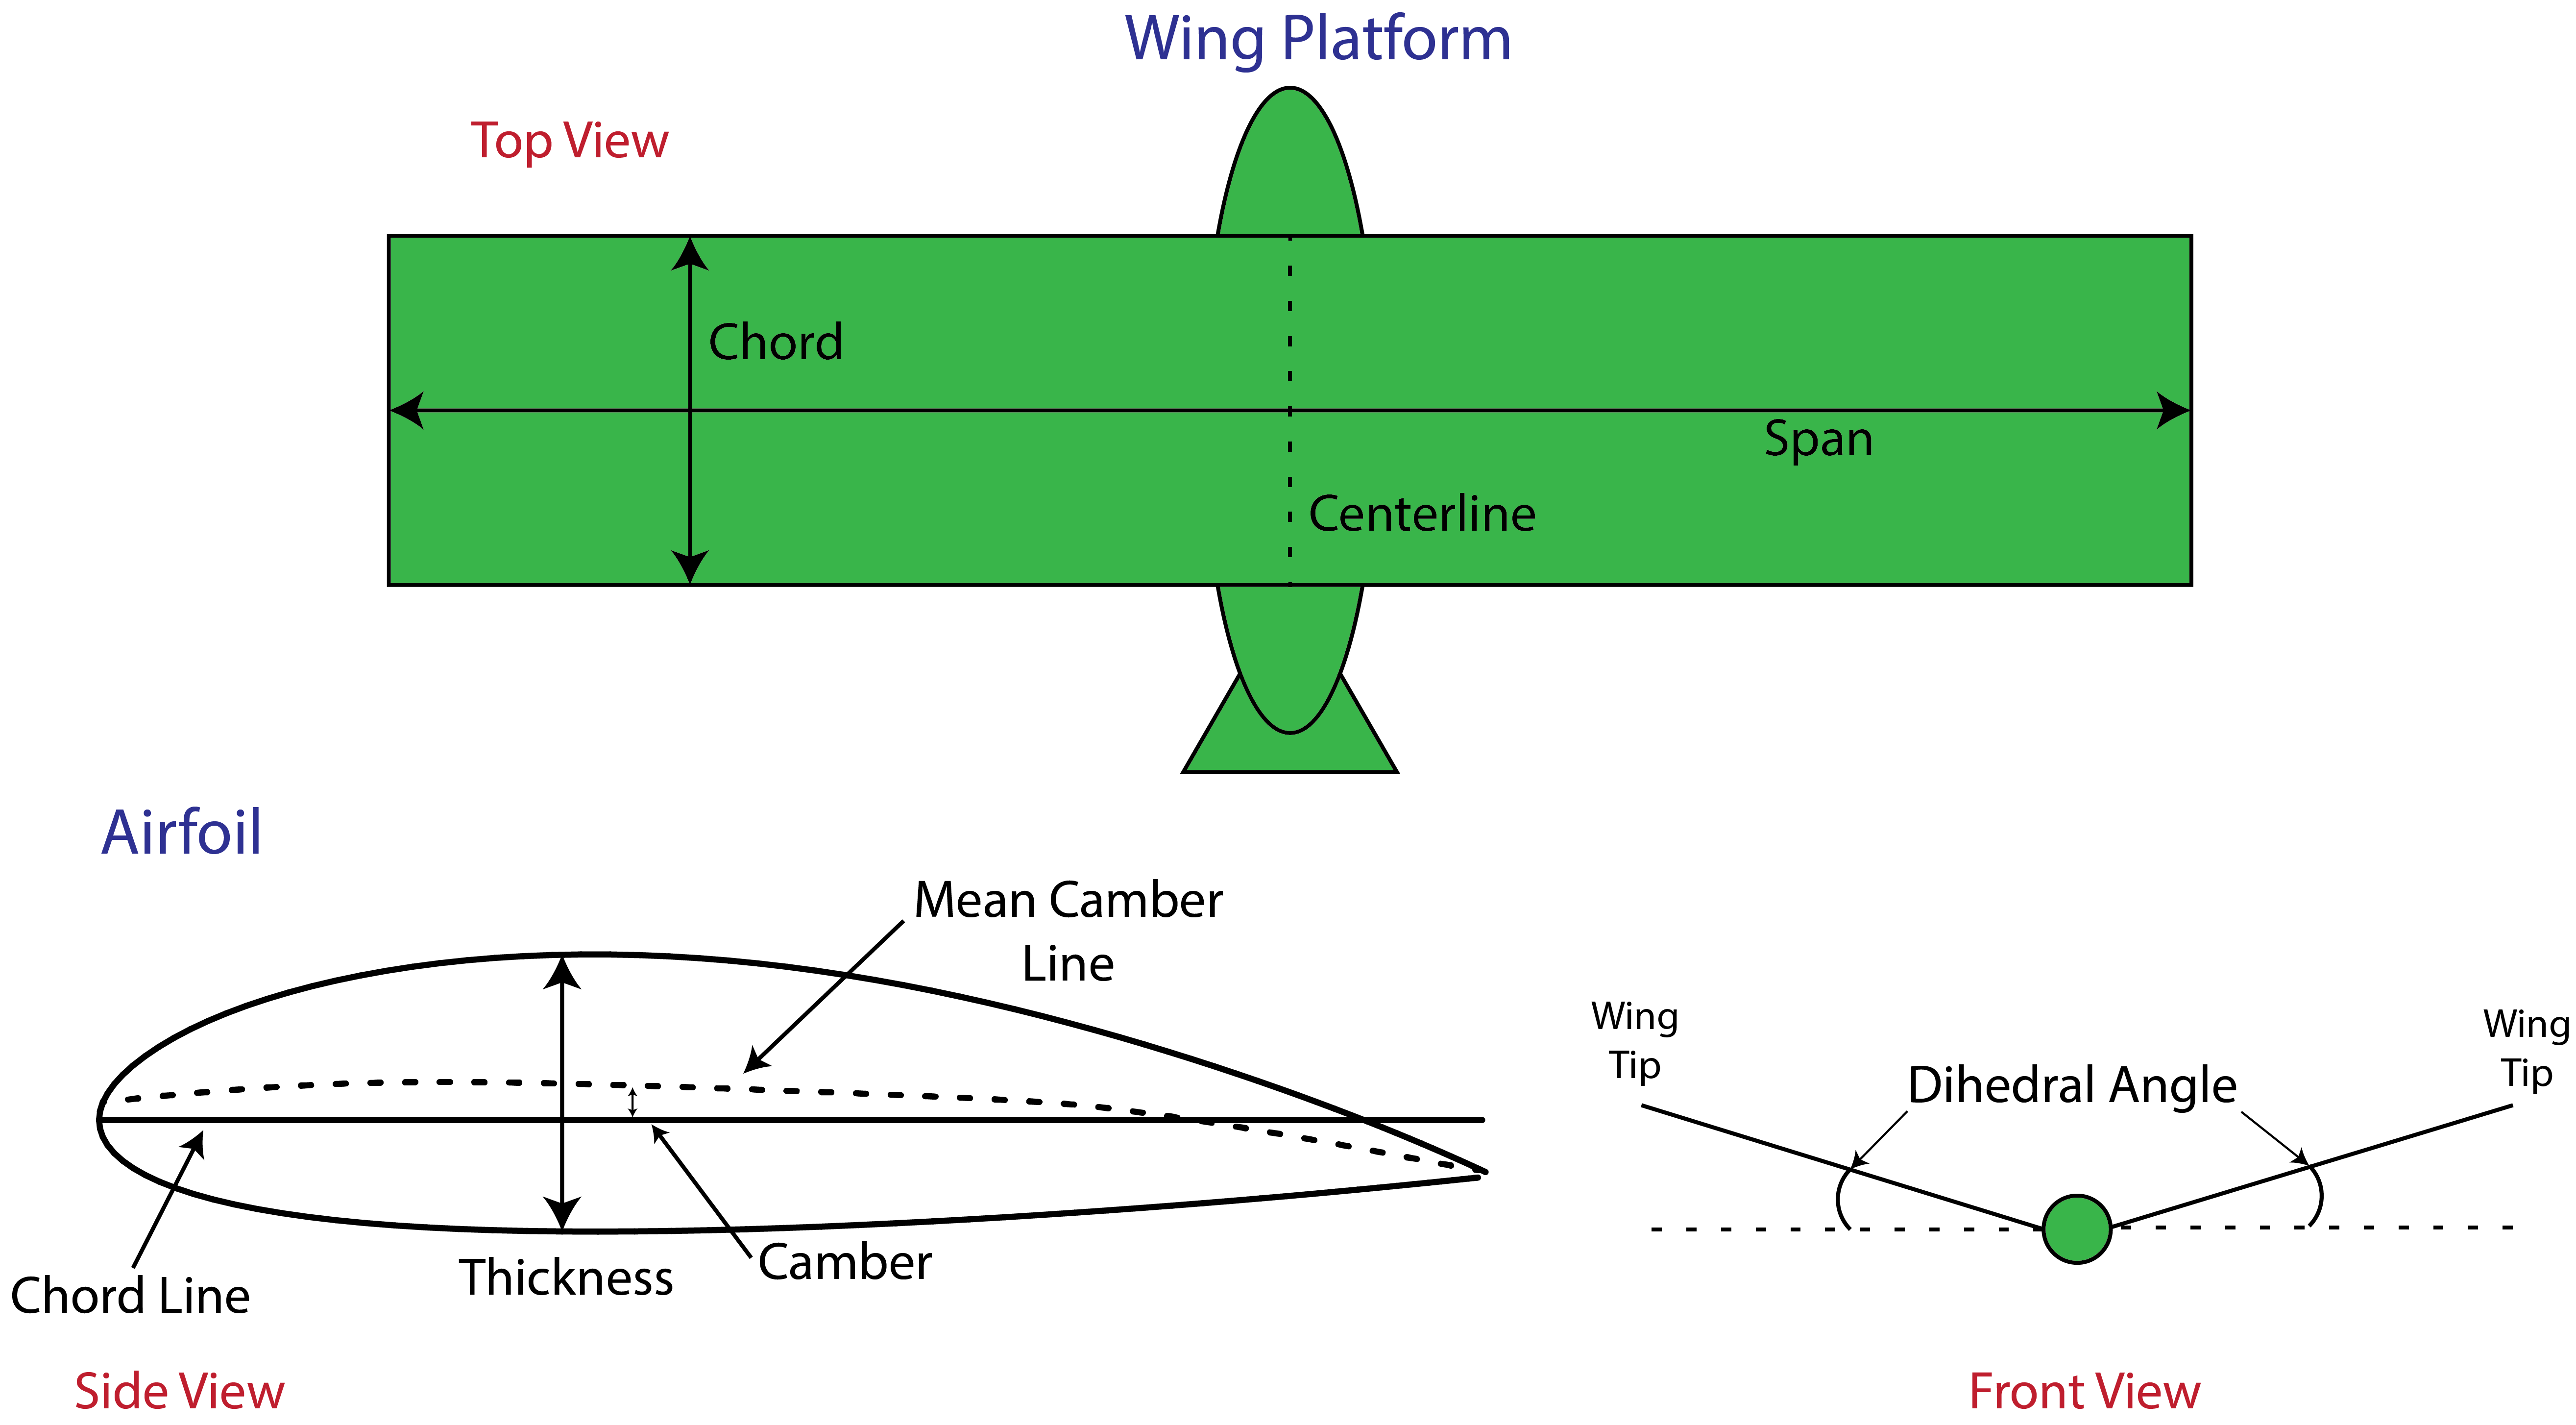
\includegraphics[width=0.75\linewidth]{./Figures/AirCraftGeometry-01.png}
\caption{General definitions of aircraft geometries, this is a recreation of a figure provided by NASA Glenn Research Center}
\label{fig:airGeo}
\end{figure}

Shape morphing typically achieves the increase in aerodynamic efficiency by changing the aircraft geometry to become more optimal at various flight conditions. Typical fixed wing aircraft are designed to have maximum efficiency around their nominal cruise conditions, which necessarily results in the design being sub-optimal at other flight conditions. In theory the aircraft should spend the vast majority of it's flight time at its nominal cruise condition but due to things like weather, airspace congestion, and distance of flight this is not always true and shape morphing can help address this problem.  

There are four major challenges associated with making shape morphing a viable technology for the industry, distributed high-power density actuation, structural mechanization, flexible skins, and control law development. \cite{reich2007introduction} Of these primary challenges we will be addressing the control law development but the linkage between all of these challenges will be evident. I will specifically be focusing on the development of reasonable models, control and capability analysis of an active twist aircraft. Wing twist is defined as the angle that the wing tip is compared to the angle that the wing meets the aircraft body as shown in Figure \ref{fig:twist}. Wing twist was selected because it is capable of generating many interesting and potentially important phenomena for increased efficiency.

\begin{figure}[thpb]
\centering
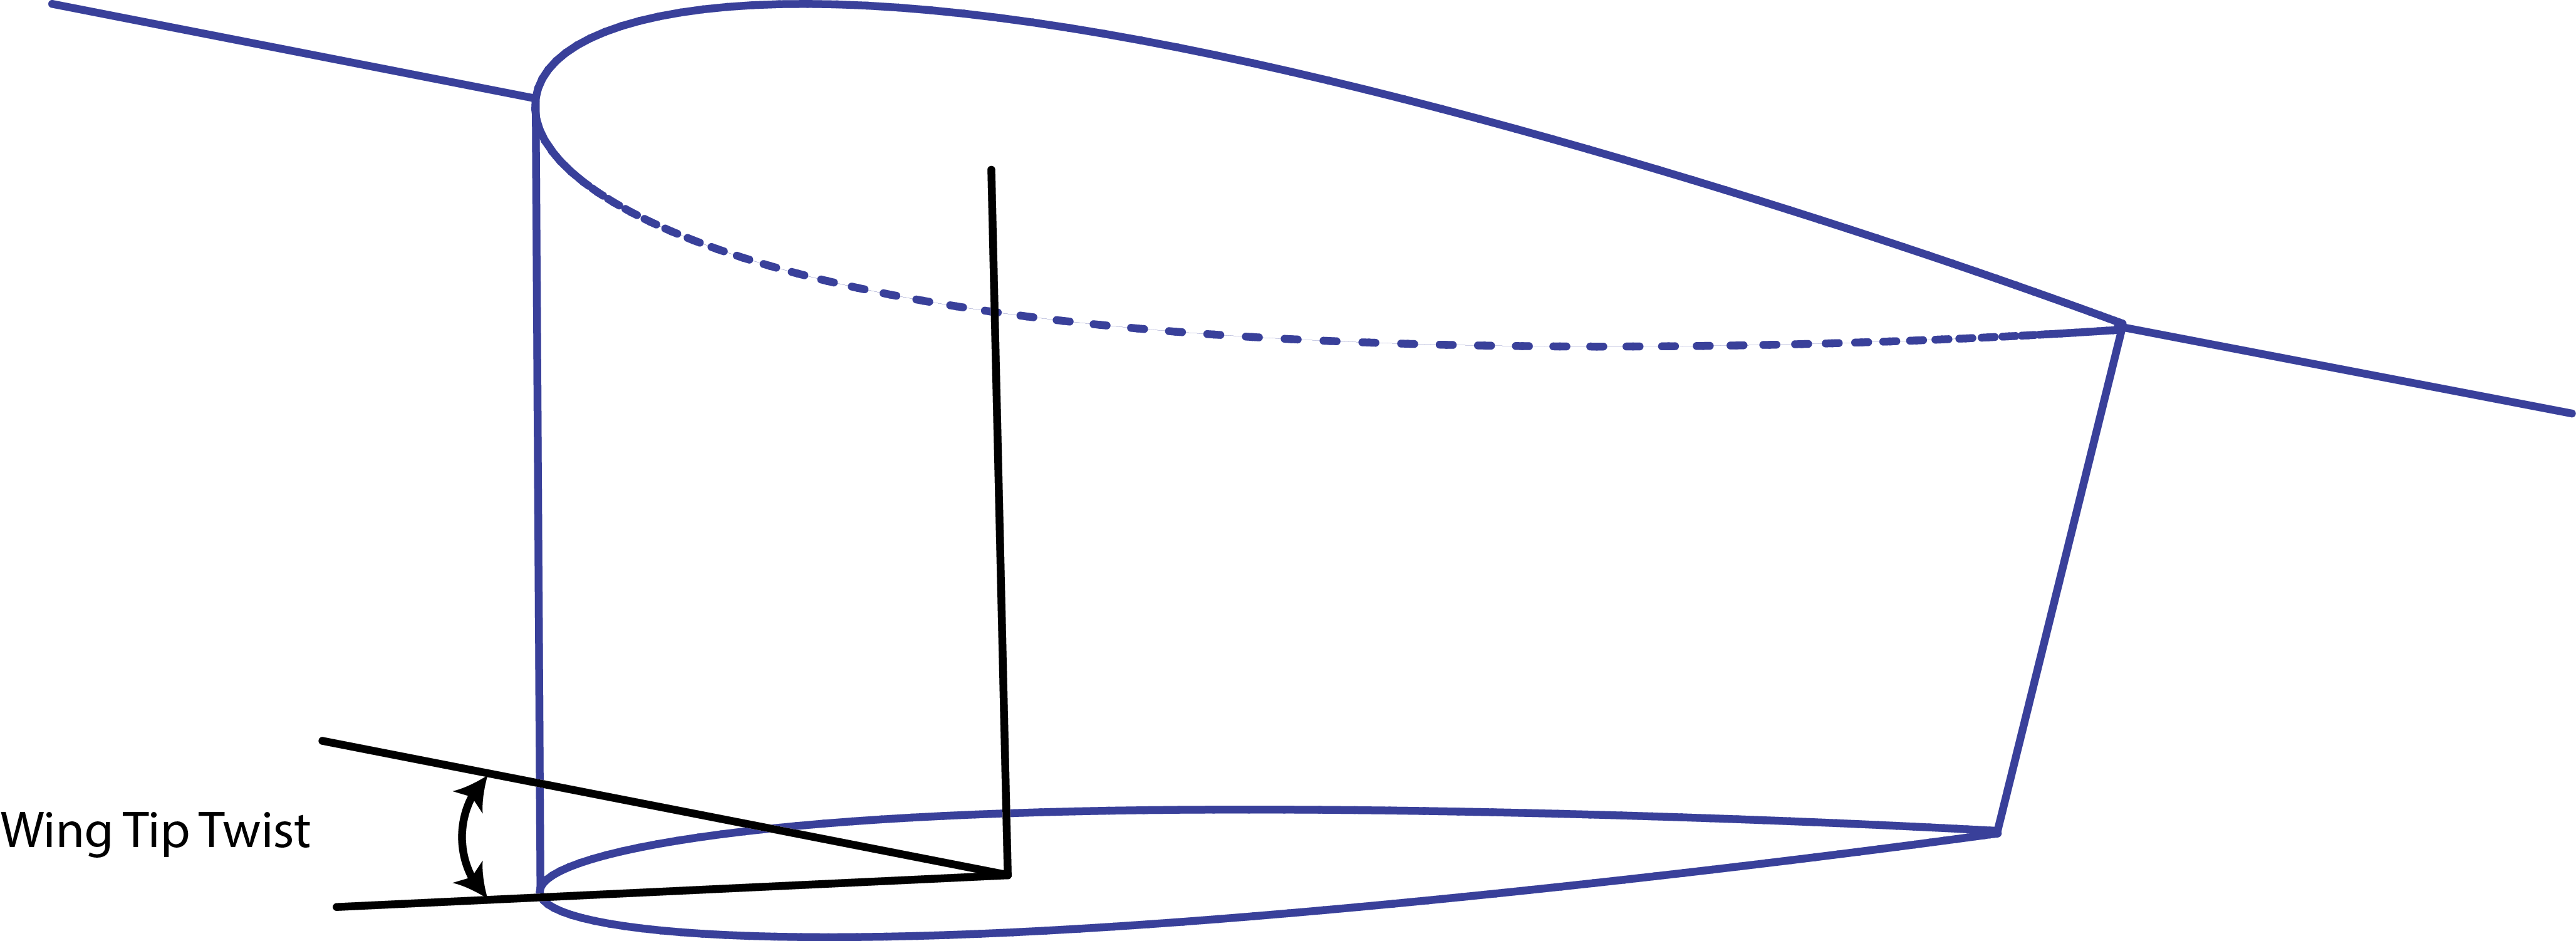
\includegraphics[width=0.75\linewidth]{./Figures/WingTipTwist.png}
\caption{Definition of wing twist, where the tip of the wing is twisted at an angle different than the one that the wing meets the plane body at}
\label{fig:twist}
\end{figure}

\section{Applications}
\label{sec:applications}
Our motivation example focused primarily on commercial aircraft but the application space for this research can be broken down into three area, where commercial aircraft are but one part.
\begin{itemize}
\item Commercial Aviation - The commercial aviation sector was touched on above but effective control of active twist could have a direct and immediate impact on this field. A very effective use of wing twist could be the creation of active twisting winglits that can be trimmed to optimal wash out of various flight regimes. This could provide significant performance increases during take-off and landing.
\item Military Aircraft - The military has a desire to have an aircraft that is flexible to a multitude of missions. The use of active twist technology would allow for more efficient vehicles and longer flights but more crucially would increase the performance envelope of the aircraft. It could be especially important as an enabling technology for other high efficiency designs such as blended body and flying wings where the minimum stability margin of the aircraft can be catastrophically affected by the discontinuities that come from traditional flaps.
\item Unmanned Aerial Vehicles (UAVs) - UAVs have a lot of promise as means of delivery or inspection but one of the primary problems is that the rotocopter set-up that is ideal for these missions has sever longevity issues while the fixed wing variant need long ranges to take off and land and are difficult to loiter in the same spot. The active twist technology could help by decreasing the loiter speed and loiter radius of the UAV while also decreasing the range necessary to take off and land.
\item High Altitude Long Endurance (HALE) Aircraft - Active twist for HALE aircraft have many of the same advantages as commercial aviation but they also have a distinct advantage of not typically having passengers. This means that it is possible for the HALE to take advantage of some of the aerodynamic efficiency gains of active that can be seen in flapping flight that would be untenable for passengers.
\end{itemize}

\section{Contributions of this Work}
In this work we try to take a holistic approach to the design and analysis of the active twist controllers as such there are some varied contributions to the field which are listed below.

\begin{itemize}
\item Development of an aeroelastic simulation method that is specifically tailored to the targeted operating regime. 
\item Design of wind tunnel tests to access the broader capabilities of the technology and validate the simulation.
\item Creation of decentralized control expanding on the work of Siljak \cite{siljak2011decentralized} to address the issues associated with overlapping decentralized control.
\item Expansion of the concept of the transfer matrix method as a means of control centered modeling and decentralized structural stabilization.
\item Explored the use of aerodynamic database for structural state estimation and inner loop active twist control.
\end{itemize}

%%%%%%%%%%%%%%%%%%%%%%%%%%%%%%%%%%%%%%%%%%%%%%%%%%%%%%%%%%%%%%%%%%%%%%%%%%%
\chapter{Background}
\section{Aeroelastic Modeling}
\label{sec:aeroMoldLit}

Aeroelasticisity has been a well known and well studied problem sense shortly after the creation of planes.   To date many of the studies use some combination of an aerodynamic simulator that then couples with the mode shapes and the wing. Indeed Nguyen et. al. \cite{nguyencoupled} use an elastic wing model, a vortex lattice program (Vorview), and a geometry modeling tool coupled together to create an aeroelastic model. The elastic wing modeling utilizes twist, flapwise and chordwise bending as well as having the bending-torsion coupled included. The eventually simplify by neglecting the chordwise bending because it is noted that it is small, especially in comparison to the wing sweep angle.

The aeroelastic angle of attack is defined to be the velocity of wind in the chordwise direction over the velocity in the flapwise direction. These velocities are a combination of the air speed and the elastic velocities. The forces resulting from the aeroelastic angle of attack are calculated by using the aeroelastic angle of attack and the lift and pitching moment coefficients as calculated by Vorview.

The static and dynamic analysis were performed by galerkin method to separate the mode shapes for each given natural frequency. The static uses the analysis of the primary mode with no dynamics and is added to the dynamics modes. Each state equation is the result of the summation of a primary set of modes and then the states are converted into the modal coordinates are used for the calculations.

In \cite{nguyen2012aeroelastic} the work from \cite{nguyencoupled} is extended. Nguyen et. al present variable camber continuous trailing edge (VCCTE) flat system to control the wing twist and wing bending in order to shape the wing. The proposed wing would be shaped into the optimal configuration for drag reduction during cruising and possibly lift enhancement during take off. The VCCTE would consist of an three component flap to dynamically shape the the mean chord of the airfoil to change the aerodynamic center location and the spanwise variation in lift.

The generic transport model (GTM) was used as the basis of the rigid body model. The aeroelastic equations were derived for the wings using primarily the adjusted local angle of attack and the lift, drag, and moment coefficients associated with the instantaneous wing configuration. The beam model used was the same that was used in \cite{nguyencoupled} with the addition of bending-torsion coupling and the inclusion of cordwise bending. The GTM has jet engines attached and the affects of the thrust from the engines on the wings was also considered, as was the fact that fuel is stored in the wings resulting in the wing density, area moment of inertia, and the bending torsion constants.

The rigid body mechanics an the aeroelastic equations associated with the wings were coupled via the integration of the local lift, drag and moments along the span. This was important because the frequencies of the aeroelastic and rigid body components are close and coupled. The equations of motion take the form of a time varying state space model. A observer is proposed to estimate the local angle of attack and then a LQR control was proposed to minimize the drag, states and control.

With many of the same assumptions and that Nguyen et. al. work on Wang et. al presented a reduced modal approach to modeling nonlinear aeroelastic responses in flexible wings in \cite{wang2014nonlinear}. They also presented $H_{\infty}$ control for the trim from the reduced modal model. The wing was treated like a typical beam system to get the expected modes then the amplitude of the modes were used to generate that dynamics which was then reduced. The dynamic modal equation relates linearly the natural frequencies to the modal amplitudes and the interaction between the modal amplitudes as well as the external forces.

The aerodynamics forces were calculated using a 2-D unsteady airfoil theory to develop lifting, drag, and moment coefficient with respect to angle of attack. The local angle of attack is generated from the proportion of vertical velocity, resulting velocity from the angular velocity and the total airspeed with the induced angle of attack subtracted. The induced angle of attack was generated with an approximation of Theodorsen's lift deficiency function.

Due to the reduction scheme there can be some drift in the values that must be checked via a spanwise integration. The external force effects due to thrust, gust, and control surface input were converted to the modal coordinates to create the dynamics equation, which were used for the proposed control.

Getting away from the assumed mode shapes that the previous works utilized Su proposed a strain based modeling technique for a slender flexible wing in \cite{su2014modified}. The localized strain components can be integrated to arrive at the local position and positional rate components for the finite elements. To allow for warping of the system a warping field was proposed where a finite selection of warping modes for the cross sectional area and the effects of neighboring warped cross sections are considered. Then using the virtual work concept the external and internal virtual work was combined to derive the equations of motion.

\section{Morphing Wings}
Morphing wings as a means of control is an intuitive and readily understandable means of controlling an aircraft. In our daily life we often see birds flying and their primary mechanism of motion control is changing the shape of their wings. Not surprisingly then the first attempt at roll control was done via wing warping during the Wright brothers first flight. \cite{friswell2009prospects} The use of compliant wing morphing mechanisms quickly fell out of favor it seems likely this was due to the rise of the structural shell mechanism, for which the shell of the aircraft became the primary structural component. While aircrafts still used truss structures like that found in the Wright brother's plane the weight was reduced dramatically by having the shell bare the load. \cite{weisshaar2011aerospace} It seems likely that the additional engineering effort to make the shell compliant to actuation while resisting aeroloading and the relative ease at which traditional control surfaces could be manufactured resulted in the dormancy of morphing wing research.

Work on compliant morphing wings resumed in the 1980's with Air Force Research Laboratory's (AFRL) the Active flexible wing (AFW) technology project that was using traditional control surfaces to shape a compliant wing. \cite{miller1988active} This was eventually followed by the ``PARTI'' \cite{pinkerton1996controlled} and DAPRA's Smart Wing Project \cite{kudva2001overview} who used smart materials as a means of actuation for the morphing airfoil, irreversibly linking the morphing wing research to the continued development of smart materials. With the turn of the century research in morphing aircraft exploded, in the next few sections we will explore some of the more relevant morphing wing research.

\subsection{Camber Morphing}
Changing the camber of an airfoil is probably the most researched area of morphing wing research. This is because the dramatic changes that the camber can have on the aerodynamic performance. 

One of the most successful Small Business Innovation Research (SBIR) in recent memory has been FlexSys which created an variable camber trailing edge for  wings\cite{kota2009mission} and rotors\cite{kota2008adaptive}. The FlexSys system uses a underlying compliant mechanism to control the structural deformation of the airfoil and therefore the camber with a simple rotary actuator. This structure encourages a reduction of stress concentrations  and the weight  of joints while minimizing backlash. The interface between the stiff wing and the compliant trailing edge is an elastomer membrane. FlexSys was able to demonstrate the effectiveness of their variation of the camber morphing through model test flight and are currently performing full scale slight systems both of which have yielded positive results. 

The spiritual successor at AFRL to the ARW program is the AFRL Variable Camber Compliant Wing (VCCW) which shares a lot of similarities to the FlexSys system. The VCCW is focused on optimization of the variable camber design by combining the the leading and trailing edge mechanism, eliminating the need for stretchable skin, while minimizing the energy consumption. The VCCW has been exhaustively studied prior to flight testing via bench top testing and simulations \cite{miller2015fluid} as well as wind tunnel testing \cite{zientarski2015wind} both showing the expected performance increases. 

The final camber morphing project that I will highlight is NASA and Boeing's Variable Camber Continuous Trailing Edge Flap (VCCTEF). The VCCTEF bears some similarities to the AFW project in that it is using the the flaps to control the aerodynamic forces and the resultant wing shaping. This is achieved via numerous trailing edge flaps that changed the airfoil camber and are attached to each other via and elastomer filling. The flap actuation is achieved with a slow large displacement using Shape Memory Alloy (SMA) and faster electric drive motors for the outboard flap.\cite{urnes2013mission} The configuration of the actuator results in actuation constraints that much be taken into account. \cite{swei2014aeroelastic} Of the camber morphing technologies presented here the the VCCTEF project is one of the only ones that committed a significant effort to investigating the control of the aircraft\cite{nguyen2012aeroelastic} though additional validation has not been completed beyond simulations.

\subsection{Flapping Flight}
There has been a large amount of research in the area flapping flight. \cite{shyy2010recent} While the field of flapping flight field is expansive and robust we will be focusing only on the research relevant to this thesis in this section. The work relating to relevant modeling techniques are highlighted in Section \ref{sec:aeroMoldLit}. 

Much of the flapping flight research has been focused on creating bio-mimetic devices to study the flight characteristics of flying animals. A group from the Department of Integrative Biology at the University of California Berkeley, has created an dynamically scaled model of a common fruit fly's wing to study the effects of different patterns of wing strokes. They were able to show that the wing twist during the stroking motion can result in rotational circulation that they theorized can be used as a means of directional control and force modulation.\cite{dickinson1999wing} In later works they were able to show that the wing twist had a significant impact on the lift force in flight, especially when the wing strokes are of small amplitudes. They also showed that the quasi-steady estimates was limited in its capability of replicating the kinematic patterns,\cite{sane2001control} while continuing to expand on the means of quasi-static simulation techniques.\cite{sane2002aerodynamic}

There is on going work at AFRL into the control of flapping micro aerial vehicles. Much of the work has focused on the use of split-cycle control to achieve various maneuvers. \cite{weintraub2014implementation} Split-cycle control is at it's core using asymmetric cosine waves as show in Figure \ref{fig:splitCycle}, where the period and phase of the rising and falling edge are modulated to create asymmetric forces inducing 6 dof of control. The  work has been focused primarily on creating biomimetic hovering. \cite{doman2010wingbeat,oppenheimer2011dynamics}

\begin{figure}[thpb]
\centering
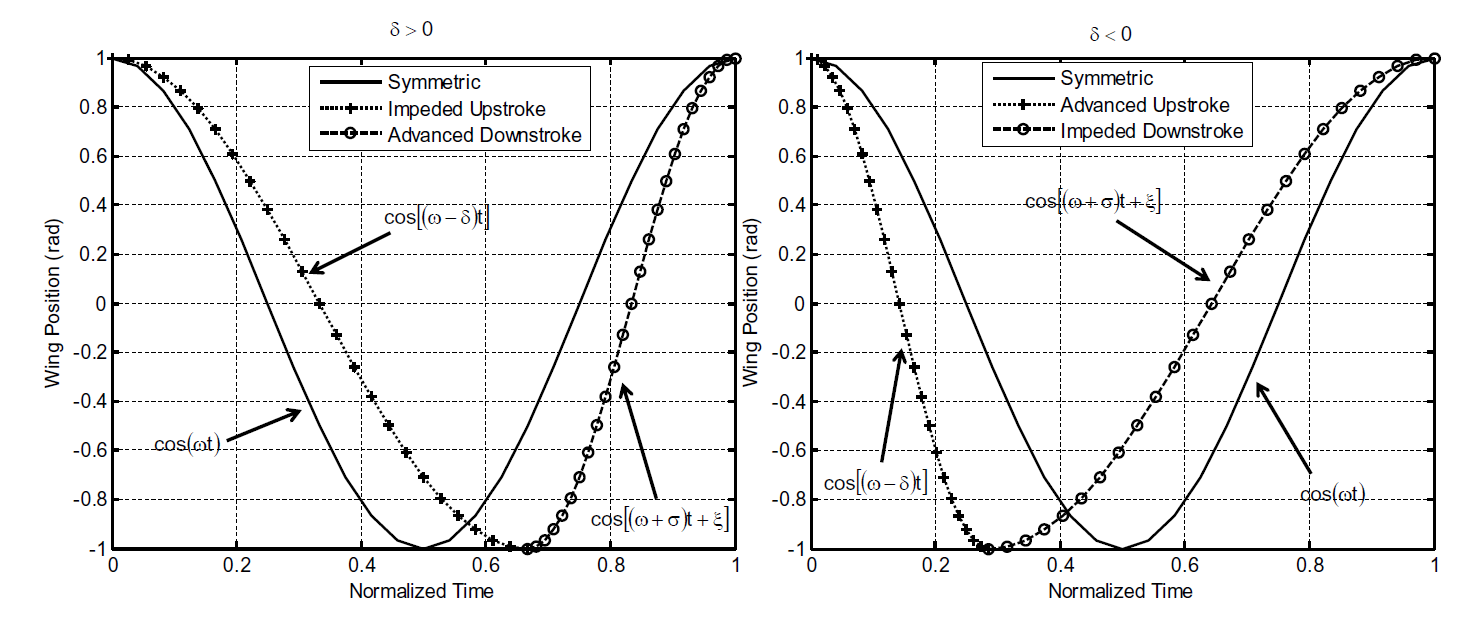
\includegraphics[width=1\linewidth]{./Figures/splitCycle.png}
\caption{Split-cycle example waveform. Figure taken from  \cite{weintraub2014implementation}.}
\label{fig:splitCycle}
\end{figure}

\subsection{Active Twist}

The research in the thesis is focused on the modeling and control of active twist aircraft making the work presented in this section of critical importance. To the authors knowledge the first known modern investigation of variable twist on a wing was performed by Ferris at NASA Langely. \cite{ferris1977wind} Ferris created an model aircraft with $35^{o}$ sweep and the ability to modulate the camber of the leading and trailing edge as well as the sectional twists. In this study the twist was implemented by having the leading edge camber morphing hinge being more swept than the trailing edge. As a result of the implementation the variable twist the affects of the twist and camber changed could not really be de-coupled and as a result only the camber was investigated.

Unlike the morphing wing field in general investigation into specific active twist technology did not begin until the mid 2000's. This is likely because the flexibility that camber morphing offers over active twist. Camber also has an conceptual advantage because modern aircraft's aileron, flaps, and slats are generally intended to replicate variable camber. Keeping that in mind much of the research that was done on active twist has been part of the creation of a fully adaptable aircraft. This is the case for \cite{neal2004design} where Neal \textit{et. al.} created a fully adaptive aircraft that was able to change it's span, sweep and tip twist. While they had created an aircraft that was capable of active tip twist when they performed the wind tunnel testing they did not report any of the results from the tip twist focusing instead on the mechanisms that would have the largest most immediate affects on lift like variable span.

One of the only studies of active twist technology that was actually flown was by Abdulrahim \textit{et. al.} \cite{abdulrahim2004flight}. They made two different small sized UAV's one with wing curling capabilities and one with wing twisting capabilities they flew both and compared the two aircraft performance. The aircraft wings are not of a typical NACA airfoil like design, instead they are more akin to reinforced membranes. The authors noted that it was difficult to achieve system identification of the curling aircraft due to time0varying asymmetries, limited data collection and data quality. They did not attempt to perform the molding on the wing twisting aircraft but it seems likely that the last two issues remained as well. They were able to show that the wing twist was an effective means of roll control.

Of the previous active twist research the most relevant to the work presented in this thesis is the work of Majji \textit{et. al.}\cite{majji2007design} at Texas A\&M and the later work of Vos \textit{et. al.}\cite{vos2010mechanism} at Delft University of Technology. Majji \textit{et. al.} developed an redundant torque tube active twist set-up where the wing box was split into one third sections with a telescoping torque rod in attaching in four places to allow for multiple combinations of twist. The wing box and torque tube was then skinned using an elastomeric skin. They used Prandtl's lifting line theory as a means to calculated the expected lift coefficient and compare it to the wind tunnel results. They noted in the paper that there were some structural issues with the design, primarily the skin ballooned and dimpled to the point that it was necessary to compensate for those issues in the calculations. They were still able to show the ability to control the lift coefficient with each twist location with the root twist location having the largest affect.

Vos \textit{et. al.}\cite{vos2010mechanism} set out to address some of the more common issues with active twist technology as were seen in \cite{majji2007design}. The basic premise was that the traditional wing box is not an effective means of inducing twist but that instead the outer shell can be viewed as a torque tube itself and the skin could be addressed by allowing the an open tube but with a control mechanism to help with the modulation of the torsional stiffness. They achieved their goal with a clever threaded rod system attached at the trailing edge of the carbon fiber reinforced skin and allowing the skin to slide freely on the ribs which could rotate freely on the spar. For modeling purposes they used both lifting line and vortex lattice code and then compared the results to wind tunnel tests. They found that the models matched the wind tunnel test relatively well especially at higher angles of attack where the lift induced drag would dominate. 

%%%%%%%%%%%%%%%%%%%%%%%%%%%%%%%%%%%%%%%%%%%%%%%%%%%%%%%%%%%%%%%%%%%%%%%%%%%
\chapter{Modeling}
\label{sec:modeling}
The appropriate modeling of the active twist wing is critical to further exploration on the capabilities of active twist. Due to the nature of active twist the structure becomes inherently aeroelastic. Aeroelasticity is the coupling of the aerodynamics, the rigid body dynamics of the aircraft, as well as the structural dynamics primarily of the wings. A conceptual diagram of this interaction can be seen in Figure \ref{fig:AEDiag}. The nature of aeroelasticy requires the development of both the structural modeling aspects and aerodynamic modeling with a special focus on the combination of the two.

\begin{figure}[thpb]
\centering
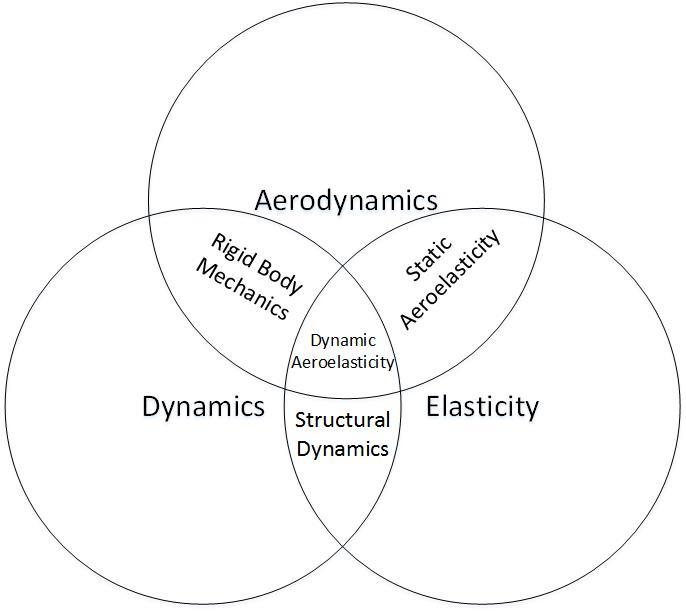
\includegraphics[width=0.4\linewidth]{Figures/AeroelasticConceptDiagram.jpg}
\caption{Conceptual diagram of the aeroelastic field. This figure is a recreation from \cite{hodges2011introduction}}
\label{fig:AEDiag} 
\end{figure}

\section{Structural Modeling}
One of the primary components of aeroelastic modeling is the structural modeling that will be coupled with the aerodynamics. I used the Galerkin finite element method (GFEM) to model the wing. The GFEM is presented in \cite{fertis1999nonlinear} the basic approach to GFEM is to use a assumed shape that takes a basic spline and use the energetic equations to populate the mass and stiffness matrix. For a standard beam bending scenario that we will be eventually extending to a wing structure a hermite cubic spline was used resulting in the assumed shape in Equation \ref{eqn:hCube}.
\large
\begin{eqnarray}
	\begin{array}{ll}
		w(x) = f_1(x)w_i +f_2(x)\phi_i+f_2(x)w_{i+1}+f_2(x)\phi_{i+1}\\
		f_1(x) = 1-\frac{3x^2}{l_i^2}+\frac{2x^3}{l_i^3}\\
		f_2(x) = x-\frac{2x^2}{l_i}+\frac{x^3}{l_i^2}\\
		f_3(x) = \frac{3x^2}{l_i^2}-\frac{2x^3}{l_i^3}\\
		f_4(x) = \frac{-x^2}{l_i}+\frac{x^3}{l_i^2}
	\end{array}
\label{eqn:hCube}
\end{eqnarray}
\normalsize

The combined use of Castigliano's theorem and Lagrange's equations of motion yield the mass, damping, and stiffness matrices, which take the general forms presented in Equation \ref{eqn:MStiff} and \ref{eqn:MMass}. 
\begin{eqnarray}
K_i = E_iI_i \begin{bmatrix} 
\frac{12}{l_i^3} & \frac{6}{l_i^2}&\frac{-12}{l_i^3}&\frac{6}{l_i^2}\\ 
\frac{6}{l_i^2}&\frac{4}{l_i}&\frac{-6}{l_i^2}&\frac{2}{l_i}\\ 
\frac{-12}{l_i^3}&\frac{-6}{l_i^2}&\frac{12}{l_i^3}&\frac{-6}{l_i^2}\\ 
\frac{6}{l_i^2}&\frac{2}{l_i}&\frac{-6}{l_i^2}&\frac{4}{l_i}
\end{bmatrix}
\label{eqn:MStiff}
\end{eqnarray}
\begin{eqnarray}
M =  \frac{\rho A}{420}\begin{bmatrix} 
156l_i & 22l_i^2&54l_i&-13l_i^2\\ 
22l_i^2&4l_i^2&13l_i^2&-3l_i^3\\ 
54l_i&13l_i^2&156l_i&-22l_i^2\\
-13l_i^2&-3l_i^3&-22l_i^2&4l_i^3
\end{bmatrix}
\label{eqn:MMass}
\end{eqnarray}

$E_i$ is the modulus of elasticity, $l$ is the length between the states, and $I_i$ is the second area moment of inertia, all of which are for the $i_{th}$ component of a beam. The stiffness matrix is the same as the damping matrix with the modulus of elasticity replaced with the damping coefficient $\eta$.When applying these matrices to to a beam like the one shown in Figure \ref{fig:Beam} each beam section generates its own matrix which add together where the beam sections share their states.
\begin{figure}[thpb]
\centering
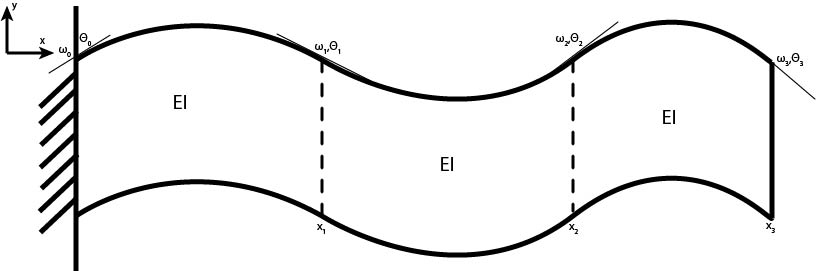
\includegraphics[width=.6\linewidth]{Figures/Beam.jpg}
\caption{Vibrating beam with states and stiffness labeled.}
\label{fig:Beam} 
\end{figure}
Extending this concept to a wing results in the configuration shown in Figure \ref{fig:CutWing}. The $Z_i$ and $\phi_{Z_i}$ are the states associated with spanwise bending which is defined as the vertical displacement along the spanwise axis. When speaking of a wing the spanwise direction is along the lateral axis. The states $X_i$ and $\phi_{X_i}$ are associated with the chordwise bending which is defined as the longitudinal displacement along the spanwise axis. The chord of a wing is the straight line connecting the leading and trailing edge of an airfoil, in Figure \ref{fig:CutWing} this is along the longitudinal axis. The final states shown are $\theta_i$ and $\phi_{\theta_i}$ which are the twist states of the wing about the lateral or spanwise axis. $n$ is the number of sections the wing is split into necessarily causing the number of sets of states to be $n+1$.
\begin{figure}[thpb]
\centering
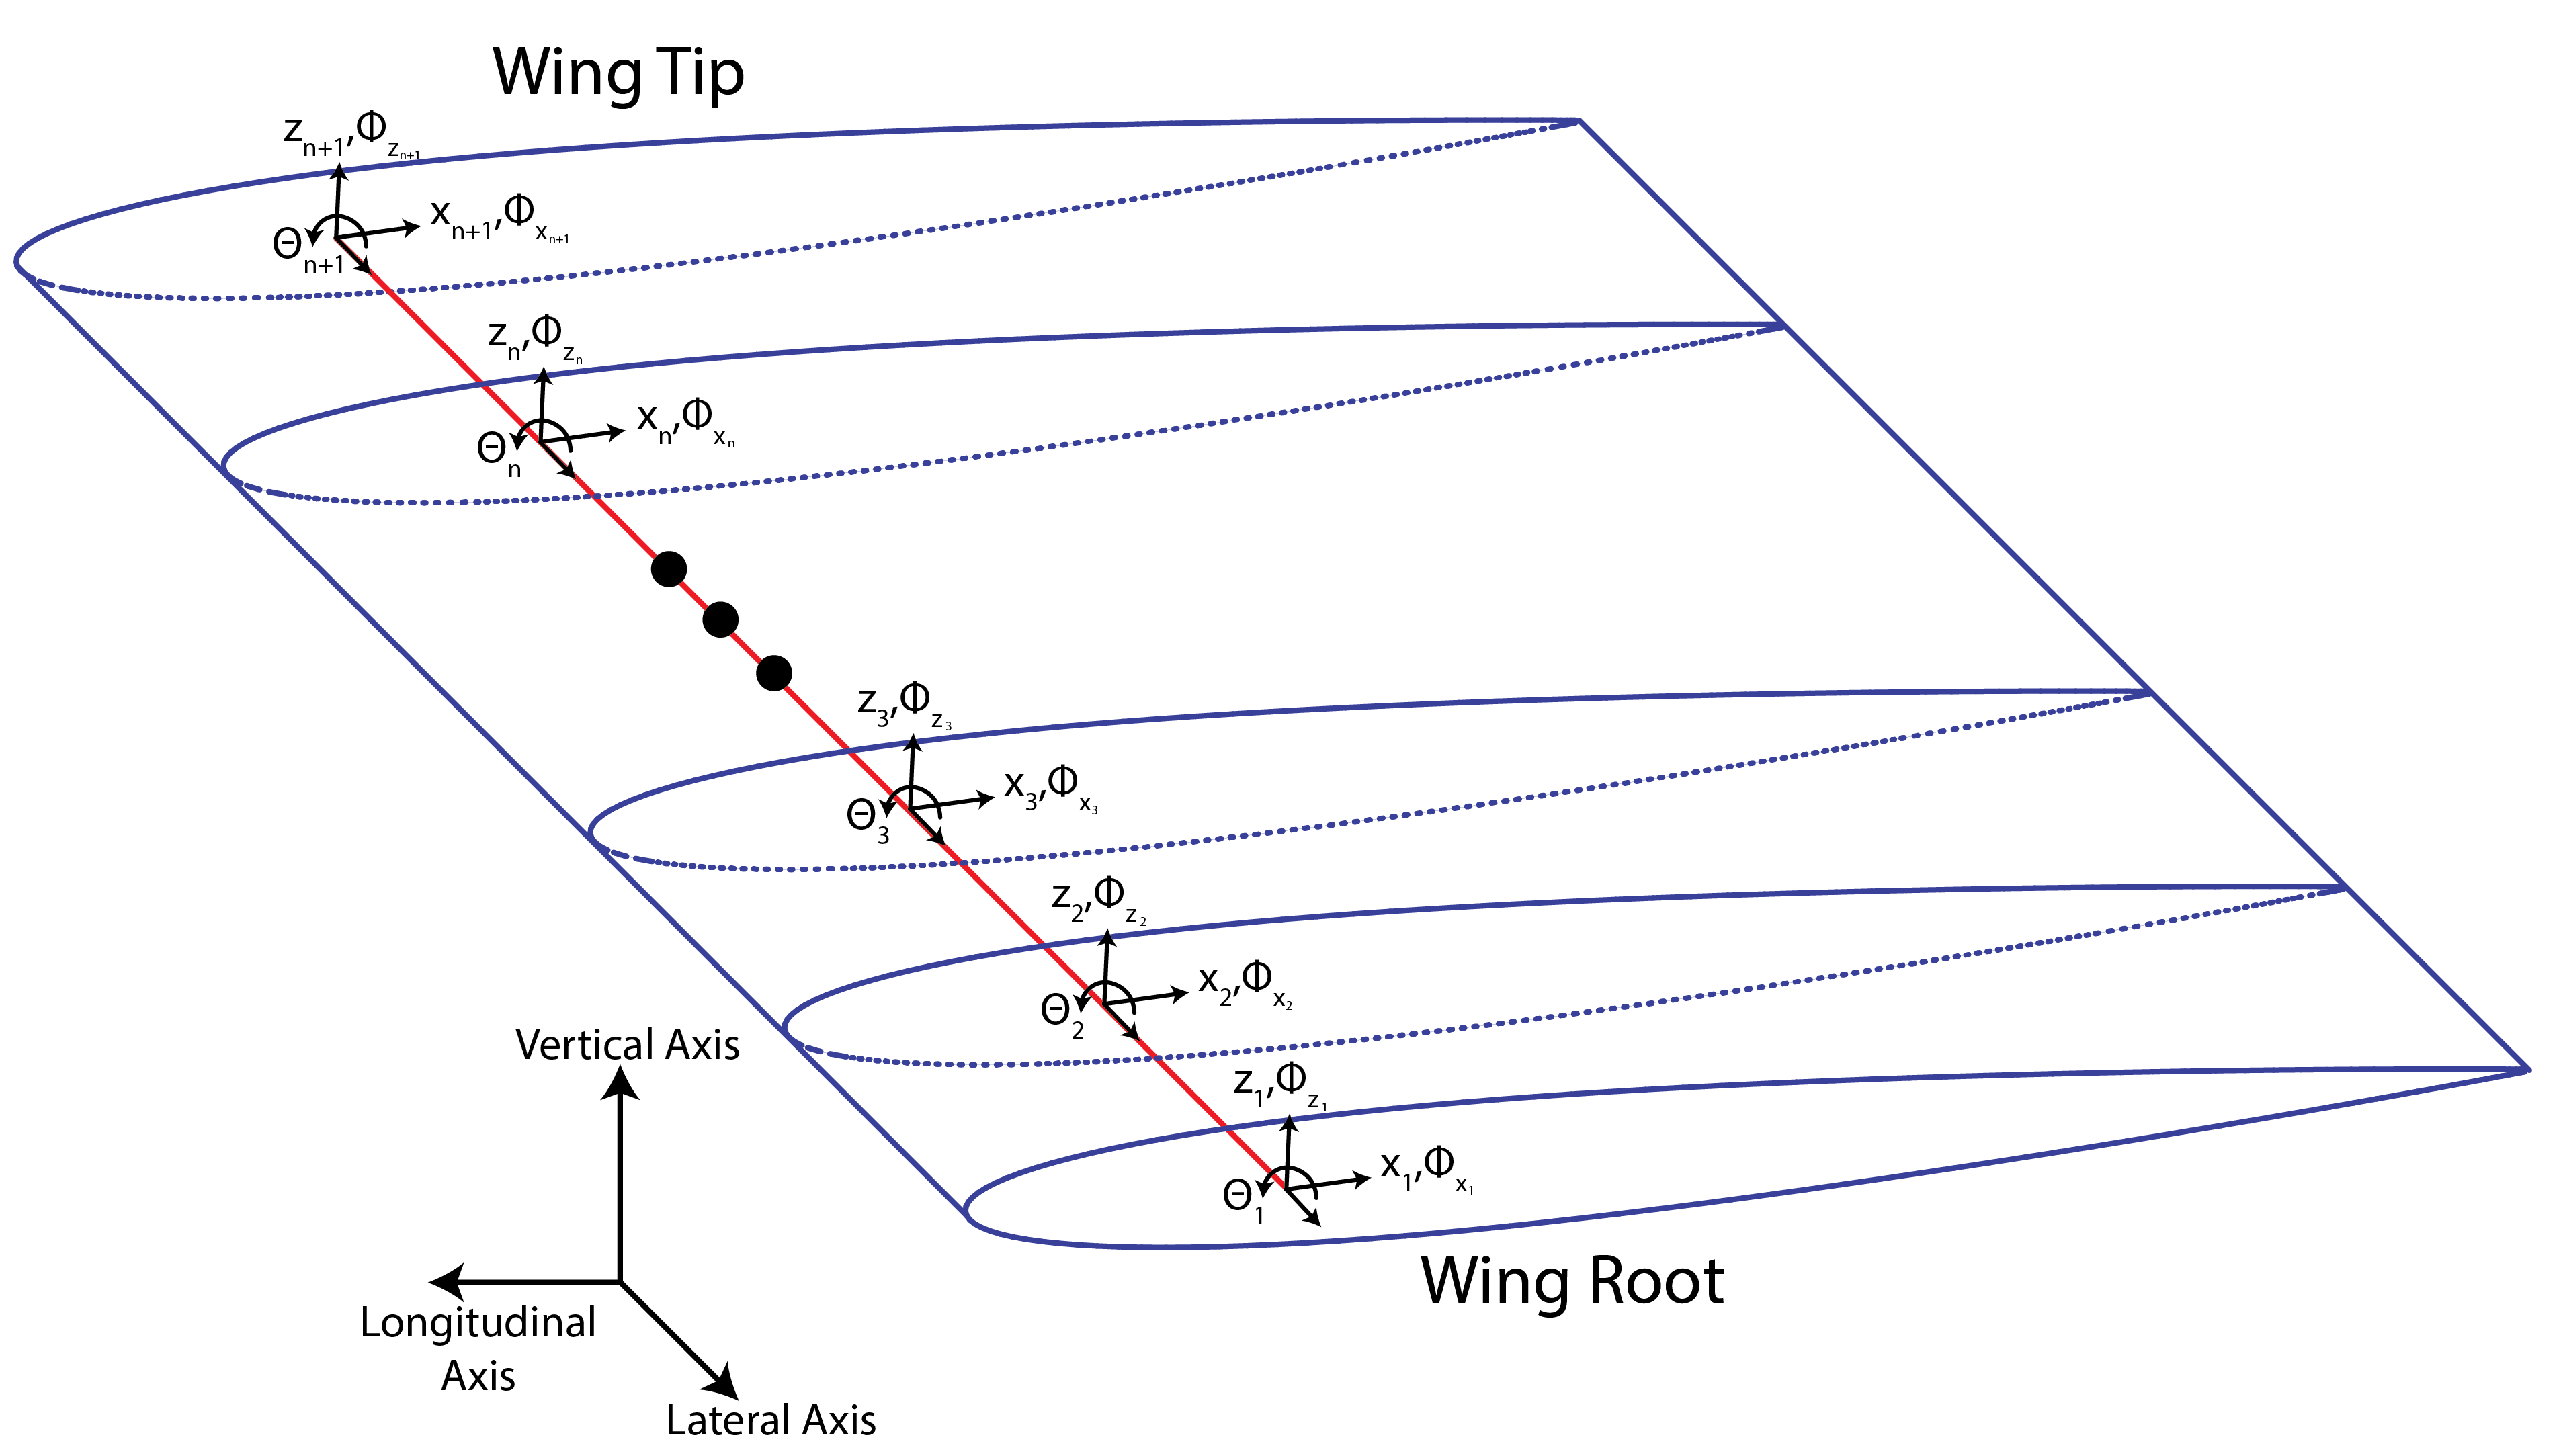
\includegraphics[width=1\linewidth]{Figures/StructuralWingStates-01.png}
\caption{Visualization of GFEM model of a wing with spanwise bending, chordwise bending and twist.}
\label{fig:CutWing} 
\end{figure}
This configuration has the dynamic equation presented in Equation \ref{eqn:GFEMeqn}
\begin{eqnarray}
X = [Z_1,\phi_{Z_1}, X_1,\phi_{X_1},\theta_1,\phi_{\theta_1}, \ldots,Z_{n+1},\phi_{Z_{n+1}}, X_{n+1},\phi_{X_{n+1}},\theta_{n+1},\phi_{\theta_{n+1}}]
\end{eqnarray}
\begin{eqnarray}
M\ddot{X}+C\dot{X}+KX = F
\label{eqn:GFEMeqn}
\end{eqnarray}
where going forward F can be populated by the aerodynamic forces.

\section{Aerodynamics}
\label{sec:aeroModel}
In order to generate the aerodynamic forces that we generated by the wing we decided to use the standard vortex lattice method. The vortex lattice method (VLM) has some distinct advantages from other methods such as lifting line theory and traditional panel methods. VLM is capable of being used on any possible geometry unlike typical lifting line theory. It also includes the interaction in the spanwise direction unlike many of the traditional panel methods. VLM is also one of the more accurate methods for simulating aerodynamic lift. \cite{bertin1998aerodynamics} The biggest disadvantage to VLM is that it does not easily lend itself to viscid calculations. Given our expected application is a meso-scale UAV the viscid affects will likely not be an issue at the operating velocities.
\begin{figure}[thpb]
\centering
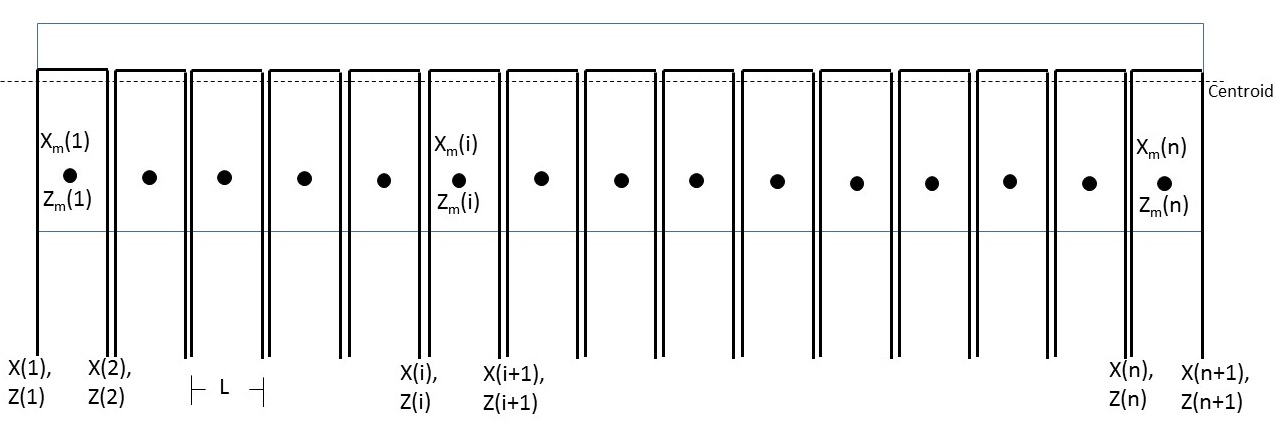
\includegraphics[width=1\linewidth]{Figures/VortexLaticeMethod.jpg}
\caption{VLM finite element horse shoe vortices with constant distances and centered about the three quarter cord line}
\label{fig:VLM}
\end{figure}

In many ways, the dynamic twist capabilities of the digital wing are similar to the most general movements that are seen in the flapping wing design. I choose to use the unsteady vortex lattice method to model the aerodynamic effects, because of its relatively low computational cost and good accuracy when presented with changing circulations \cite{long2004object,stanford2010analytical,de2012object}. The main difference between the approach proposed here and the flapping wing research is that, while most flapping flight simulations use exclusively vortex rings which propagate through time, I use horseshoe vortices. 

The expected opperating regime as shown in Figure \ref{fig:reynolds} boarders on the range where simple high reynolds number assumptions are valid but is not fully in the regime that would require the rings. This allows me to us the horseshoes because the twist sheds votices solely in the aft direction but it does so at a rate that prevents wake roll up \cite{koochesfahani1989vortical}. With the appropriate aeroelastic adjustements the horsehoes are a viable means of simulation and are prefered because of their computation efficiency. For refrence a wing with $m$ spanwise sections and $n$ chordwise sections with horseshoes would result in $3m^2n^2$ computations per a time step while for rings it would be between $4m^2n^2$ and $32m^2n^2$ computations depending on the time step and the number of chordlengths the user deems neccesary. 

\begin{figure}[thpb]
\centering
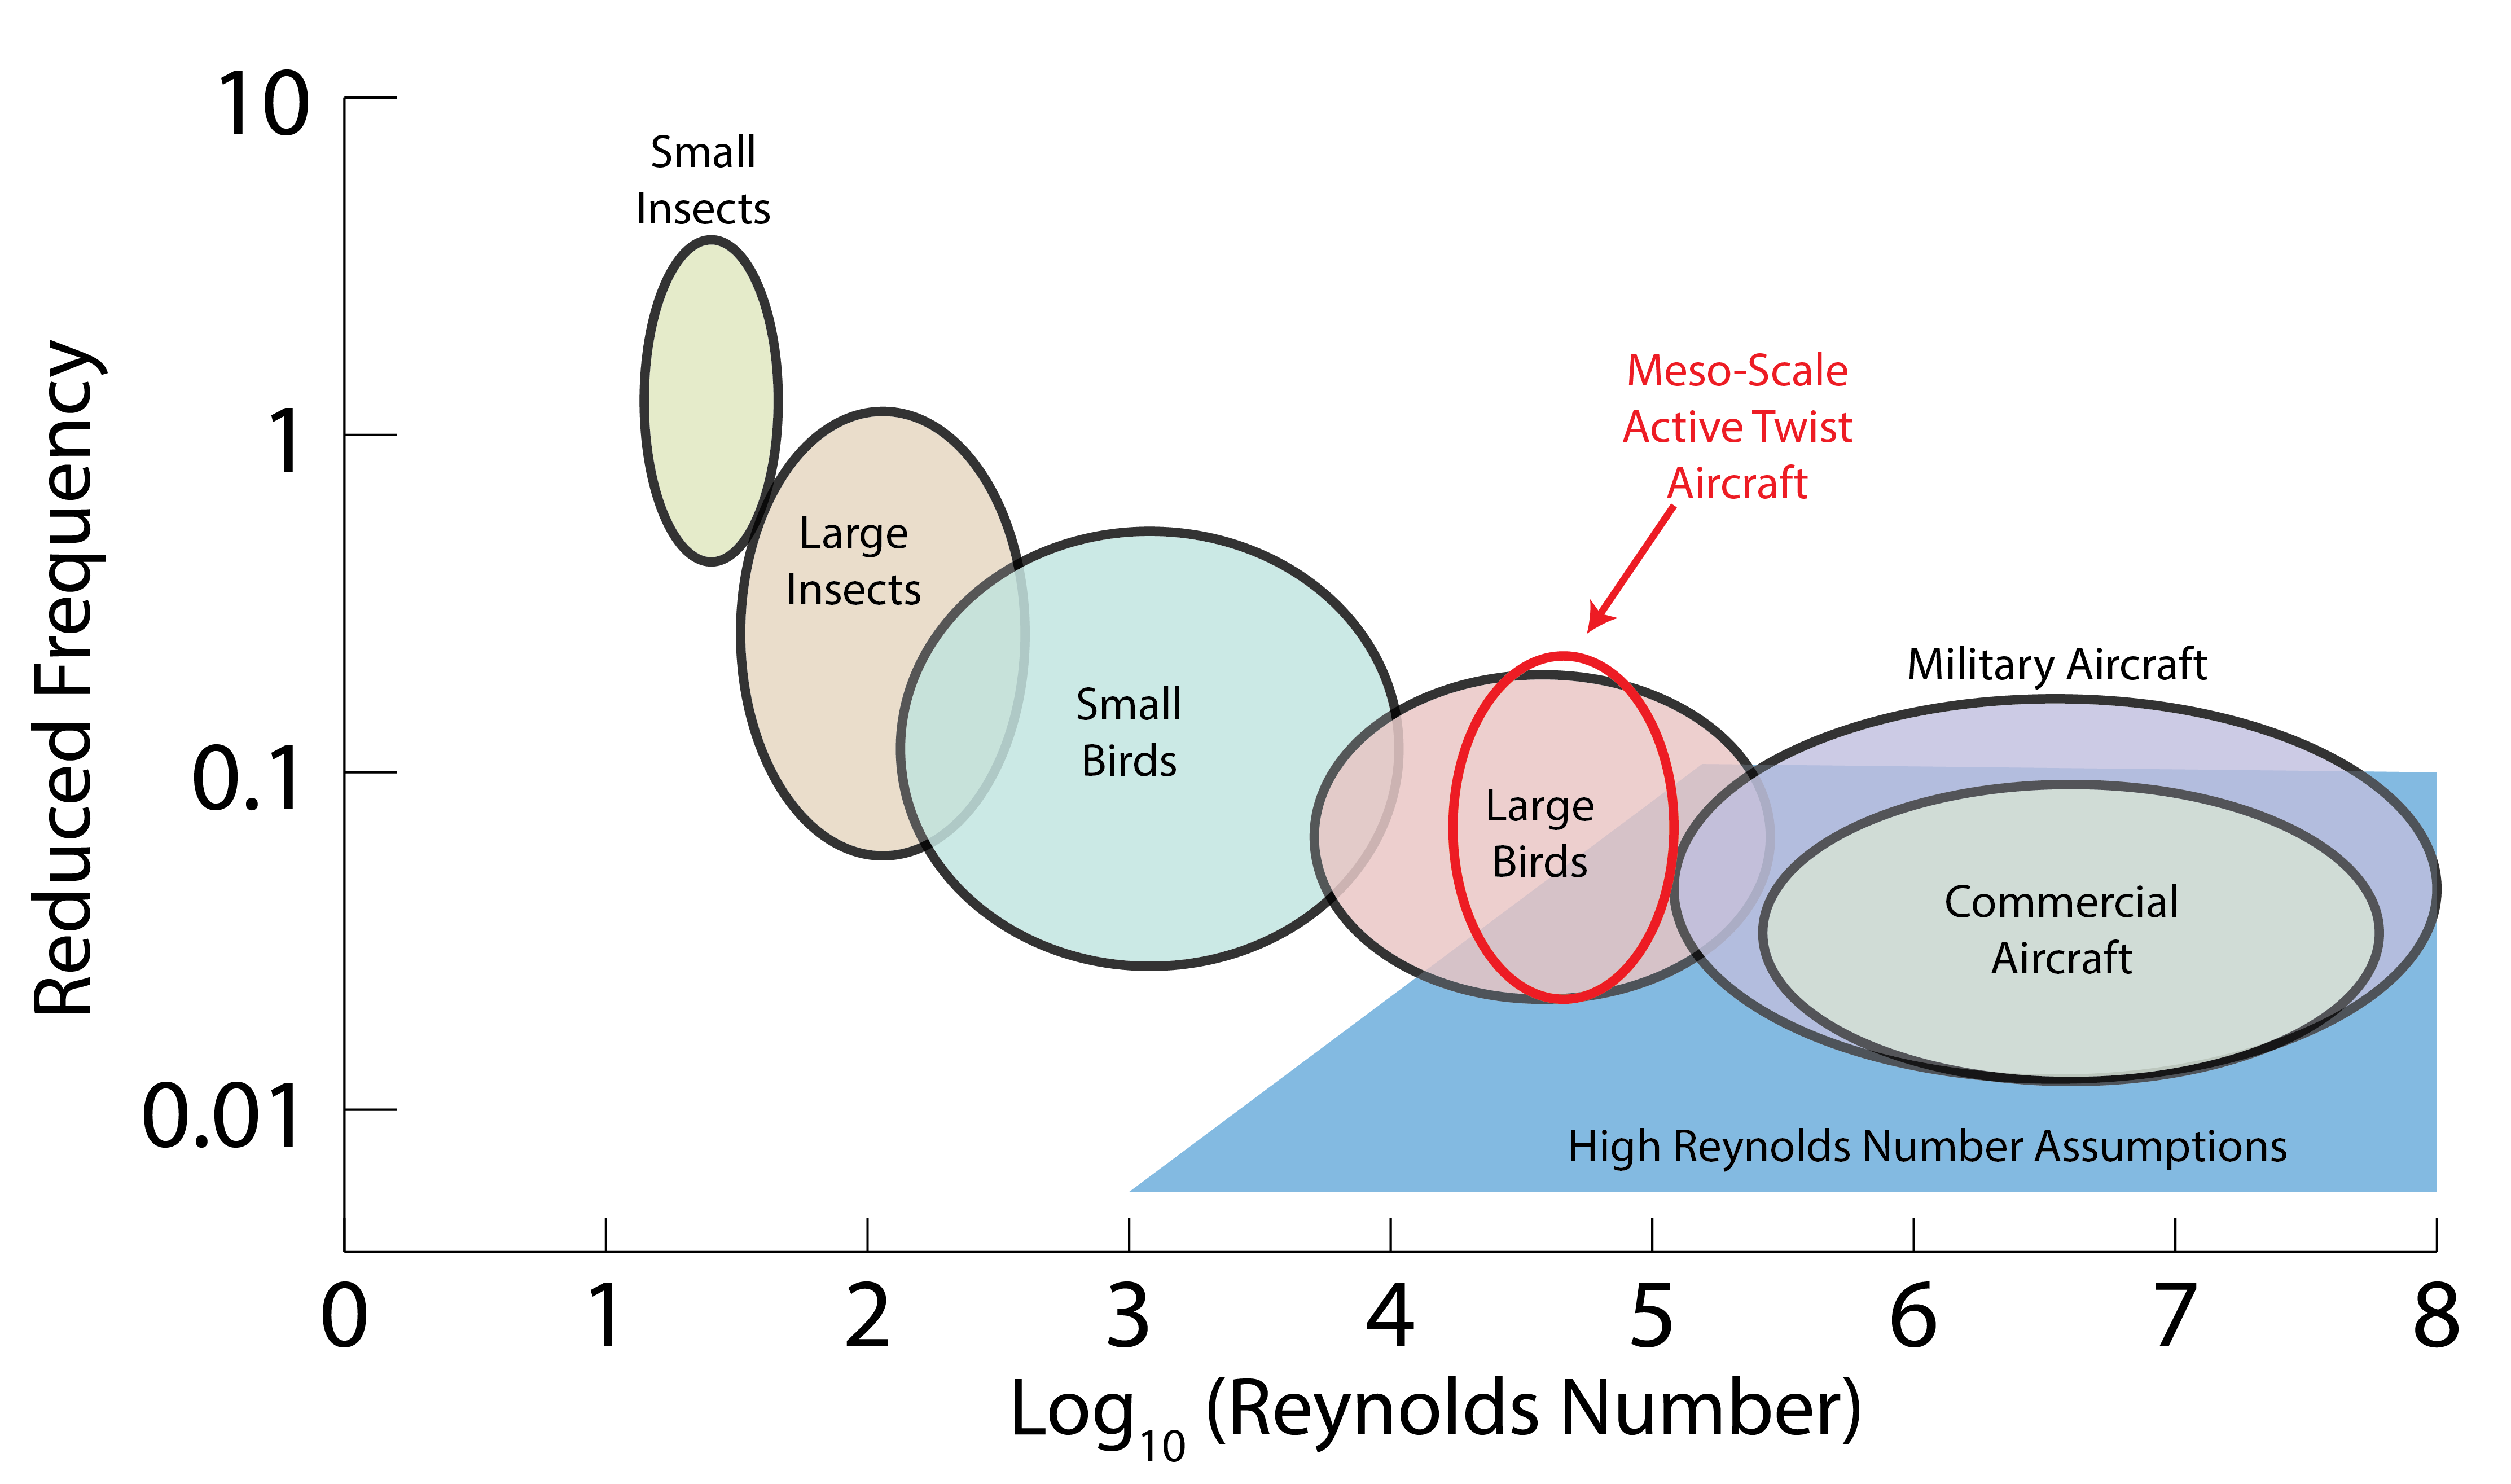
\includegraphics[width=1\linewidth]{Figures/ReducedFrequencyvReynoldsTypes-01.png}
\caption{Operating regimes of flying animals and human built aircrafts and the region where high reynolds number assumptions are applicable. The information was taken from \cite{mueller2001fixed}}
\label{fig:reynolds}
\end{figure}

These horse shoe vortices interactions is what creates the spanwise variation of the circulation about the wing. Figure \ref{fig:VLM} shows the set up for the VLM with the horse shoe vortices centered about the three quarter chord axis and the horizontal component of the horse shoe on the quarter chord axis. The horizontal vortex can be thought of as the circulation about the airfoil while the longitudinal vorticies are the trailing vortices that satisfy Helmholtz vortex theorem requiring that a bound-vortex does not change strength unless a separate vortex splits that is equal to the change in circulation. 

When comparing Figure \ref{fig:VLM} to Figure \ref{fig:CutWing} it can be seen how the VLM readily lends itself to the preexisting GFEM solid mechanics model. This was one of the reasons that the VLM was chosen to generate the aerodynamic forces, it has also already been shown to be a viable method for modeling aeroelastic effects in \cite{nguyencoupled,nguyen2012aeroelastic,nguyen2011longitudinal,nguyencoupled2014}.
\begin{figure}[thpb]
\centering
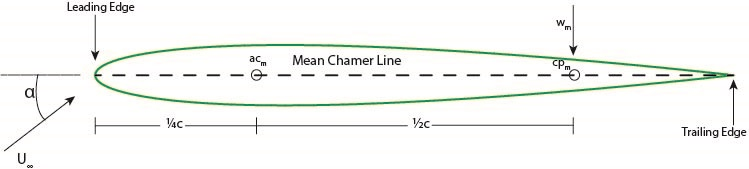
\includegraphics[width=1\linewidth]{Figures/AngleofAttack.jpg}
\caption{The angle of attack, $\alpha$, is the angle between the normal vector and the air velocity vector. For the symmetric airfoil the aerodynamic center is located at the quarter chord.}
\label{fig:alpha}
\end{figure}
While there are numerous prepackaged VLM softwares available we opted for writing a custom one primarily to have a base to build some of the proposed work that will be covered later. We based the VLM that we wrote off of the equations and methodology presented in \cite{bertin1998aerodynamics} with some auxiliary content taken from \cite{kundu2012fluid}. VLM uses Equation \ref{eqn:VLM} coupled with the boundary conditions provided in Equation \ref{eqn:VLMBC} to determine what the circulation about the airfoil is at a given control point $m$.
\begin{eqnarray}
\vec{V} = \vec{C}\Gamma_n
\label{eqn:VLM}
\end{eqnarray}
\begin{eqnarray}
-u_msin\delta cos\chi-v_mcos\delta sin\chi+w_mcos\chi cos\delta+U_{\infty}sin(\alpha-\delta)cos\chi = 0
\label{eqn:VLMBC}
\end{eqnarray}

where $\vec{V}$ is the generalized velocity vector at all the control points $m$, $\vec{C}$ is the geometry matrix that VLM generates from the current wing geometry, $\Gamma$ is the circulations at the control points. $u_m$, $v_m$, and $w_m$ are the local velocities at the control point $m$ in the longitudinal, lateral and vertical directions respectively. $U_{\infty}$ is the air speed, $\delta$ is the slope of the mean chamber line at the control point, $\chi$ is the dihedral angle, and $\alpha$ is the angle of attack. Figure \ref{fig:alpha} shows the mean chamber line which for a symmetric airfoil causes the slope of the mean chamber line, the $\delta$, to be equal to zero. Figure \ref{fig:alpha} also shows the angle of attack which is defined as $\frac{w_m}{U_{\infty}}$ where $w_m$ is the vertical induced velocity at the control point. Figure \ref{fig:airGeo} shows the front view of a wing showing the dihedral angle.

In order to combine and apply Equations \ref{eqn:VLM} and \ref{eqn:VLMBC} $\vec{C}$ needs to be generated. For each directional velocity in Equation \ref{eqn:VLMBC} a separate $\vec{C}$ can be generated by finding the velocity that each $\Gamma$ generated at a given control point. Each control point was chosen to be located at the three quarter chord and halfway between each spanwise GFEM element on the upper surface of the wing. Equations \ref{eqn:um}, \ref{eqn:vm}, \ref{eqn:wm} show how to populate the $m,n_{th}$ cell of matrix $\vec{C}$.
\begin{eqnarray}
	\begin{array}{ll}
		u_m = [(y_m-y_n)(z_m-z_{n+1})-(y_m-y_{n+1})(z_m-z_n)]/\\
		\{((y_m-y_n)(z_m-z_{n+1})-(y_m-y_{n+1})(z_m-z_n))^2\\
		+((x_m-x_n)(z_m-z_{n+1})-(x_m-x_{n+1})(z_m-z_n))^2\\
		+((x_m-x_n)(y_m-y_{n+1})-(x_m-x_{n+1})(y_m-y_n))^2\}
	\end{array}
\label{eqn:um}
\end{eqnarray}
\begin{eqnarray}
	\begin{array}{ll}
		v_m = -[(x_m-x_n)(z_m-z_{n+1})-(x_m-x_{n+1})(z_m-z_n)]/\\
		\{((y_m-y_n)(z_m-z_{n+1})-(y_m-y_{n+1})(z_m-z_n))^2\\
		+((x_m-x_n)(z_m-z_{n+1})-(x_m-x_{n+1})(z_m-z_n))^2\\
		+((x_m-x_n)(y_m-y_{n+1})-(x_m-x_{n+1})(y_m-y_n))^2\}\\
		+\frac{z_m-z_n}{4\pi((z_m-z_n)^2+(y_n-y_m)^2)}\left[1+\frac{x_m-x_n}{\sqrt{(x_m-x_n)^2+(y_m-y_n)^2+(z_m-z_n)^2}}\right]\\
		+\frac{z_m-z_{n+1}}{4\pi((z_m-z_{n+1})^2+(y_{n+1}-y_m)^2)}\left[1+\frac{x_m-x_{n+1}}{\sqrt{(x_m-x_{n+1})^2+(y_m-y_{n+1})^2+(z_m-z_{n+1})^2}}\right]
	\end{array}
\label{eqn:vm}
\end{eqnarray}
\begin{eqnarray}
	\begin{array}{ll}
		w_m = [(x_m-x_n)(y_m-y_{n+1})-(x_m-x_{n+1})(y_m-y_n)]/\\
		\{((y_m-y_n)(z_m-z_{n+1})-(y_m-y_{n+1})(z_m-z_n))^2\\
		+((x_m-x_n)(z_m-z_{n+1})-(x_m-x_{n+1})(z_m-z_n))^2\\
		+((x_m-x_n)(y_m-y_{n+1})-(x_m-x_{n+1})(y_m-y_n))^2\}\\
		+\frac{y_m-y_n}{4\pi((z_m-z_n)^2+(y_n-y_m)^2)}\left[1+\frac{x_m-x_n}{\sqrt{(x_m-x_n)^2+(y_m-y_n)^2+(z_m-z_n)^2}}\right]\\
		+\frac{y_m-y_{n+1}}{4\pi((z_m-z_{n+1})^2+(y_{n+1}-y_m)^2)}\left[1+\frac{x_m-x_{n+1}}{\sqrt{(x_m-x_{n+1})^2+(y_m-y_{n+1})^2+(z_m-z_{n+1})^2}}\right]
	\end{array}
\label{eqn:wm}
\end{eqnarray}

These equations represent the application of Biot-Savart law to the horse finite element horse shoes. The substitution of Equations \ref{eqn:um}, \ref{eqn:vm}, \ref{eqn:wm} into Equations \ref{eqn:VLM} and \ref{eqn:VLMBC} yield a system of equations that can be solve simultaneously by matrix inversion. 

Equations \ref{eqn:um}, \ref{eqn:vm}, \ref{eqn:wm} are the closed form solution for an vortex line going to infinity but it is not neccesary to calculate beyond seven wing spans due to the inverse squared components of the equation. I used an adaptation of Tornado that uses the finite solution to the Biot-Savart law for its computational speed and flexibility.\cite{melin2000vortex}

\section{Aeroelastic}
Form a practical implementation perspective sense in the GFEM axial stretching and compressing were ignored all the components associated with $y$ are constant. The other variables $z$ and $x$ vary with the spanwise and chordwise deflections presented earlier. With the control points being placed between the GFEM states and allowing the edges of the horse shoe's to be placed on the GFEM states the amount of control points can be taken from $\lfloor \frac{2(n+1)}{5}\rfloor$ for having a control point and the edges of the horse shoe placed at GFEM states to $n$. The control point spanwise and chordwise deflections can be estimated with the cubic spline from Equation \ref{eqn:hCube} and then added to the initial geometric parameters of the wing to generate $z_m$ and $x_m$.

The exchange of position vectors between the solid mechanics and the aerodynamics does not represent the totality of the coupling in an aeroelastic system. Indeed the primary means of interaction between the two components if the aerodynamic forces that are applied to the wing. Utilizing the vortex lattice method we were able to generate the circulation at each control point. The circulation directly correspond to the lift and vortex induced drag forces as show in Equations \ref{eqn:liftF} and \ref{eqn:dragF}.
\begin{eqnarray}
l(y) = \rho_{\infty}U_{\infty}\Gamma(y)
\label{eqn:liftF}
\end{eqnarray}
\begin{eqnarray}
d(y) = tan(\theta(y)+\alpha_{root})l(y)
\label{eqn:dragF}
\end{eqnarray}
where $\theta$ is the twist of the wing at a given location $y$ and $\alpha_{root}$ is the angle of attack at the root of the wing. It is assumed that the air velocity is constant in the spanwise direction. Due to the fact that the control points are placed between GFEM states the force due to circulation does not directly apply to the state equation presented in \ref{eqn:GFEMeqn}. To address this we simply split the forces equally to each adjacent states. The generated force vector can then be put into Equation \ref{eqn:GFEMeqn} to complete the current iteration of this aeroelastic modeling.

The coupling of the aerodynamic states to the structural states allows for the creation of a static aeroelastic simulation tool, which is useful especially in the preliminary design and development stages but in some cases it is necessary to have a full dynamic aeroelastic model using an unsteady vortex lattice method. 

The wing is divided into $m$ panels and calculate the aerodynamic forces/moments at each panel. Furthermore, we assume that the sectional element defined earlier coincides with the panel section, and we define $q$ collocation points around each panel section. 

\begin{figure}[thpb]
\centering
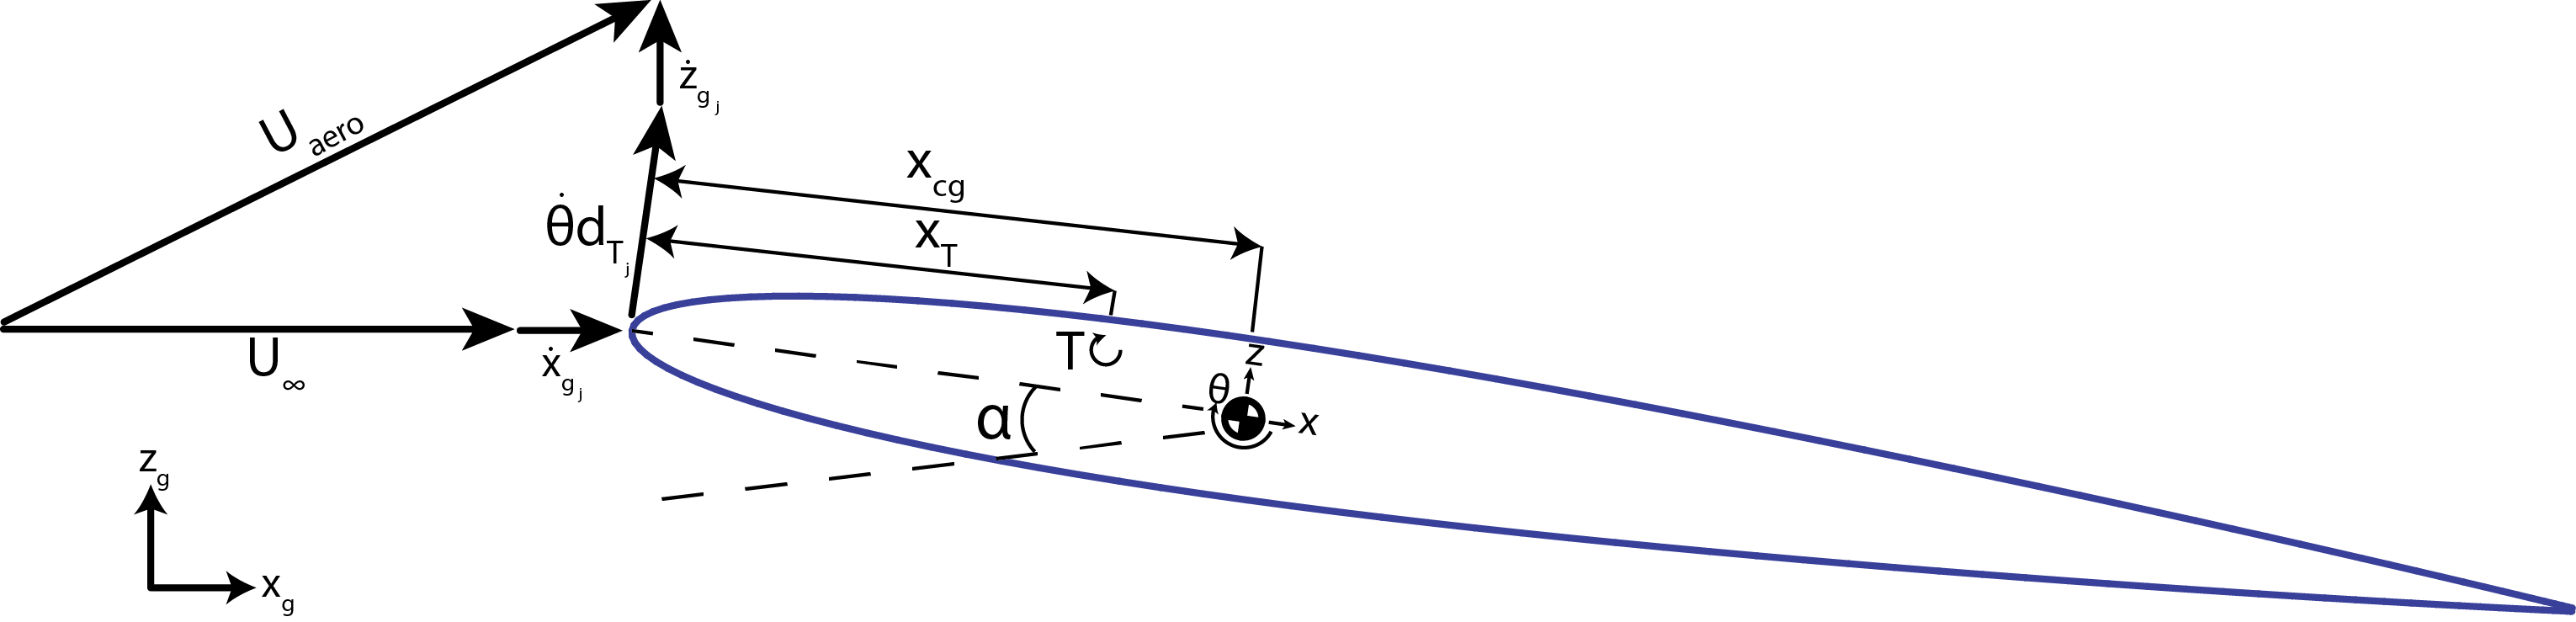
\includegraphics[width=1\linewidth]{Figures/FullAeroelasticDefinitions.png}
\caption{Aeroelastic definitions}
\label{fig:def}
\end{figure}

The local aeroelastic wind velocity vector at each collocation point can be given by
\begin{equation}
U_{i,j} = R(\alpha_{root})\begin{bmatrix}U_{\infty} \;\; 0\end{bmatrix}^T +  R(\theta_{i})\begin{bmatrix}\dot{\theta}_{i} |d_{j}| \;\; 0\end{bmatrix}^T + \begin{bmatrix}\dot{x}_{i,j}\;\; 0\end{bmatrix}^T + \begin{bmatrix}0\;\; \dot{z}_{i,j}\end{bmatrix}^T
\label{eqn:Uinf}
\end{equation}

for $ \,,\;i=1,\cdots, m\,,\;j=1,\cdots, q$ where $R(\cdot)$ denotes a $3\times 3$ rotational matrix, $\alpha_{root}$ is the angle of attack at the wing root, $U_{\infty}$ is the airspeed, $|d_{j}|$ is the magnitude of the position vector $d_{j}$ from torque tube axis to collocation point $j$, $\theta_i$ is the twist angle at $i$th panel, and $\dot{\theta}_i$ its rate, $\dot{x}$ is the rate of chordwise displacement, and $\dot{z}$ is the rate of spanwise displcacement. We should note that the local wind velocity $U_{i,j}$ defined in (\ref{eqn:Uinf}) is a tall matrix of dimension $mq \times 3$. To simplify the subsequent presentation, we rewrite its notation to be just $U_i$, where $i=1,\cdots,mq$. Then, the local aeroelastic angle of attack at each collocation point can be determined by
\begin{equation}
\alpha_{i} = \tan^{-1} \left (\frac{U_{iz}}{U_{ix}} \right) \,,\;i=1,\cdots, mq
\label{eqn:alpha_aero}
\end{equation}

Similarly, the local sideslip angle at section $i$, $\beta_i$, is given by 
\begin{equation}
\beta_{i} = \tan^{-1} \left (\frac{U_{iy}}{U_{ix}} \right) \,,\;i=1,\cdots, m
\label{eqn:beta_aero}
\end{equation}
where $U_{iy}$ is the $y$ component of $U_i$.

where $U_{ix}$ and $U_{iz}$ denote the $x$ and $z$ components of $U_{i}$. 

The circulation equation can be solved in its standard form as \cite{melin2000vortex}
\begin{equation}	\label{eqn:RHSGamma}
\left \{
\begin{array}{rll}
C_x \, \Gamma_x & = & B_x \\
C_y \, \Gamma_y & = & B_y \\
C_z \, \Gamma_z & = & B_z
\end{array}
\right .
\end{equation}
where $\Gamma_x$, $\Gamma_y$, and $\Gamma_z$ are the vectors of dimension $mq$ and denote the circulation of $mq$ collocation points in $(x,y,z)$ coordinates. The matrices $C_x$, $C_y$, and $C_z$ contain entries of influence coefficients that result form the geometry of the horseshoe vortex on collocation points in $(x,y,z)$ coordinates. The details on the influence coefficient matrix can be found in \cite{melin2000vortex}. Furthermore, the boundary conditions ${\bf B} = [B_x \;\; B_y \;\;B_z]$ are given by

\begin{equation}
{\bf B}_{i} = \begin{bmatrix}U_{ix}\cos(\alpha_{i})\cos(\beta)\\ -U_{iy}\cos(\alpha_{i})\sin(\beta)\\ U_{iz}\sin(\alpha_{i})\end{bmatrix}^T \,,\;i=1,\cdots,mq
\label{eqn:BC}
\end{equation}
where $\alpha_i$ is given in (\ref{eqn:alpha_aero}) and $\beta$ is the aircraft sideslip angle. Let ${\bf \Gamma} = [\Gamma_x \;\; \Gamma_y \;\;\Gamma_z]$, then we can solve for ${\bf \Gamma}_i$ by substituting (\ref{eqn:BC}) into (\ref{eqn:RHSGamma}). Therefore, the total aerodynamic forces and moments on the digital wing can be derived from each panel as %given collocation points can be solved by
\begin{equation}
% \begin{array}{l}
F = \rho_{\infty} \sum_{i=1}^{mq} ({\bf B}_i \otimes {\bf \Gamma}_i)
\label{eqn:aeroForce}
\end{equation}
and
\begin{equation}
M = \rho_{\infty} \left [ \sum_{i=1}^{mq} (d_i-m_c) \otimes ({\bf B}_i \otimes {\bf \Gamma}_i)\,\right ]
\label{eqn:aeroMoment}
\end{equation}
where $\rho_{\infty}$ is the air density, $d_i$ the $i$th collocation point position vector, $m_c$ the position vector to the center of gravity, and $\otimes$ denotes the vector cross product. It should be noted that the sectional aerodynamic forces and moments from (\ref{eqn:aeroForce}) and (\ref{eqn:aeroMoment}) are coupled with the structural dynamics described in (\ref{eqn:GFEMeqn}). Finally, the total aerodynamic lift ($L$), drag ($D$), and lateral force ($S$) can be given by 
\begin{equation}
\begin{bmatrix}D\\S\\L\end{bmatrix} = R(\alpha_{root})R(\beta)\begin{bmatrix}F_{ax}\\F_{ay}\\F_{az}\end{bmatrix}
\label{eqn:LDS}
\end{equation}
where $F = [F_{ax} \;\;F_{ay} \;\; F_{az}]^{T}$.   

%%%%%%%%%%%%%%%%%%%%%%%%%%%%%%%%%%%%%%%%%%%%%%%%%%%%%%%%%%%%%%%%%%%%%%%%%%%
\chapter{Active Twist Wing Design}
For the development of the control of an active twist wing it is necessary to have a platform to work from. For this purpose we have two different active twist wings designs that were made by two different collaborators. The first active twist wing is a lattice-based design that was informed wing simulations to create a holistic design process and was manufactured by collaborators at NASA Ames. The second active twist wing is an polystyrene hollow core design created by collaborators at Aurora Flight Sciences.

\section{Composite Lattice-based Cellular Structure Active Twist Wing Design}

The ability of composite lattice-based cellular structure to form complex geometries with anisotropic material properties is an enabling technology for morphing wing flight. Figure \ref{fig:plane} shows the active twist wing mounted in the wind tunnel with the actuation mechanism highlighted.

\begin{figure}[thpb]
\centering
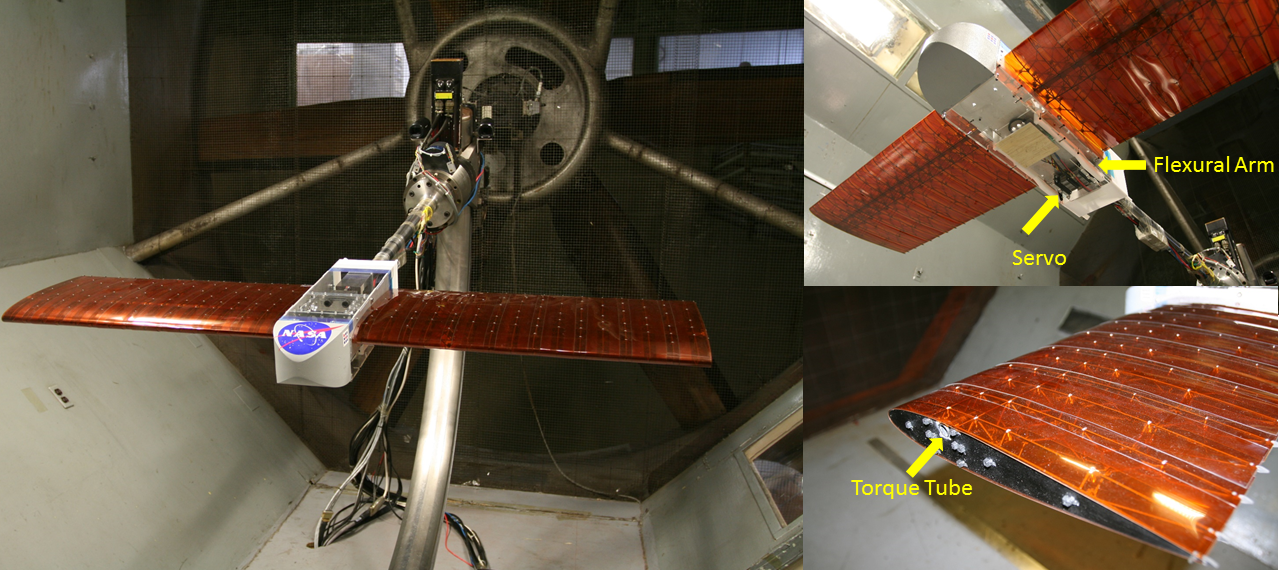
\includegraphics[width=1\linewidth]{./Figures/Plane.png}
\caption{Wind tunnel test setup for a digital wing model.}
\label{fig:plane}
\end{figure}

With any wing application where it is potential for large displacements there is a common problem with the skin of the wing. The wing skin is the layer that has direct contact with the air. The problem with wings that have large displacements is that instabilities in the skin result in buckling and ridges or dimpling of the skin, all of which increase the friction and therefore drag of the plane. A more recent approach has been proposed to make the skin be applied in sections with the bending and twist allowances coming from the joints.

One of the necessary steps to doing this is to determine the size of a given patch that will not result in significant displacement of the skin during normal operating conditions. To address this problem we combined the VLM method we presented earlier with the standard panel method Xfoil. Figure \ref{fig:PPFlow} shows the flow chart representing the combination of VLM and Xfoil where VLM coupled with the GFEM result in a lift coefficient that is then passed to Xfoil. Xfoil then generates a pressure profile for each spanwise lift coefficient that was generated by the VLM.
\begin{figure}[thpb]
\centering
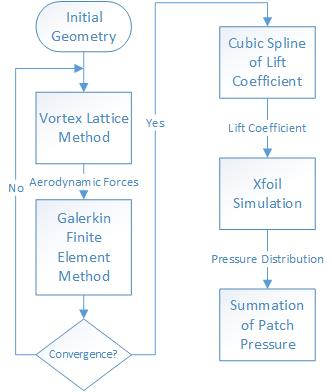
\includegraphics[width=0.3\linewidth]{Figures/PatchPressureFlowChart.jpg}
\caption{The initial geometry is given to the VLM which generates the aerodynamic forces that are then passed to the GFEM for static analysis. If the geometry that results from the GFEM converges then a cubic spline is used to create a lift coefficient for every millimeter. Those lift coefficients are then passed to Xfoil which generates the pressure distribution around the airfoil for each section.}
\label{fig:PPFlow}
\end{figure}

In order to determine the necessary size of the patch the maximum pressure is assumed to the be the center of the patch. The pressures generated by Xfoil  within the specified patch size are summed for each pressure profile generated from independent lift coefficients within the specified patch size. Figure \ref{fig:PProfile} shows the average patch pressure with respect to angle of attach and patch size. The shape of the curve is not symmetric about the zero angle of attack because as the angle of attack is negative the induced drag changes direction. Figure \ref{fig:PatchDisp} shows the maximum displacement normalized for material and geometric constants, of a patch plotted against the patch size and angle of attack. The patch displacement was determined using the navier solution to the Kirchoff-Love plate theory assuming that the average pressure from Figure \ref{fig:PProfile} is constant across the patch. Since the wing can be assumed to be a flat plate in many situations this assumptions should be valid as well and result in equation \ref{eqn:KLPlate}.
\small
\begin{eqnarray}
w(x,y)D = \sum_{m=1}^{\infty}\sum_{n=1}^{\infty}\frac{16P_0}{(2n-1)(2m-1)\pi^6}\left[\frac{(2m-1)^2}{a^2}+\frac{(2n-1)}{b^2}\right]^{-2}\frac{sin(2m-1)\pi x}{a}\frac{sin(2n-1)\pi y}{b}
\label{eqn:KLPlate}
\end{eqnarray}
\normalsize

where,
\begin{eqnarray}
D = \frac{2h^3E}{3(1-\nu)}
\end{eqnarray}
where, $h$ is the depth of the plate, $E$ is the modulus of elasticity, and $\nu$ is poisson's ratio. It is desirable to have the largest possibly patch size possible prior to the normalized displacement values becoming dependent on angle of attack. Figure \ref{fig:PatchDisp} shows this to be around $30mm$. 
\begin{figure}[thpb]
\centering
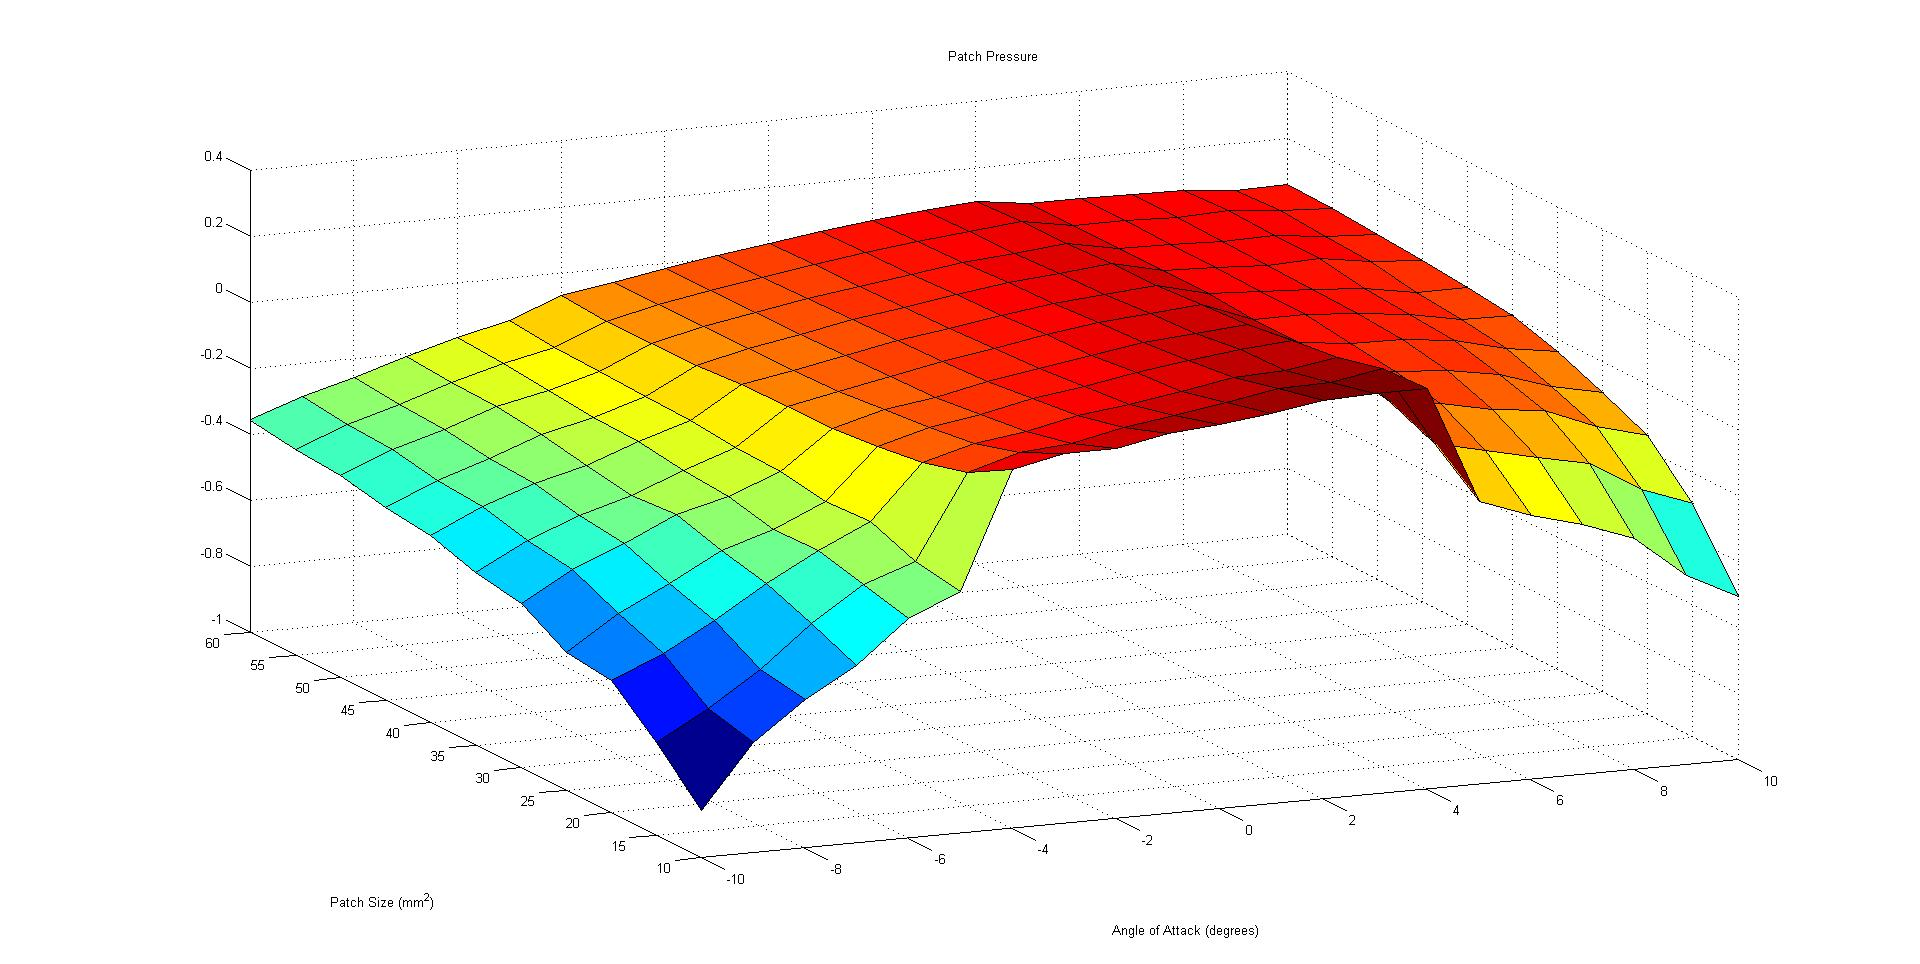
\includegraphics[width=1\linewidth]{Figures/FreePatchPressure.jpg}
\caption{The average patch pressure plotted against the angle of attack and patch size.}
\label{fig:PProfile}
\end{figure}
\begin{figure}[thpb]
\centering
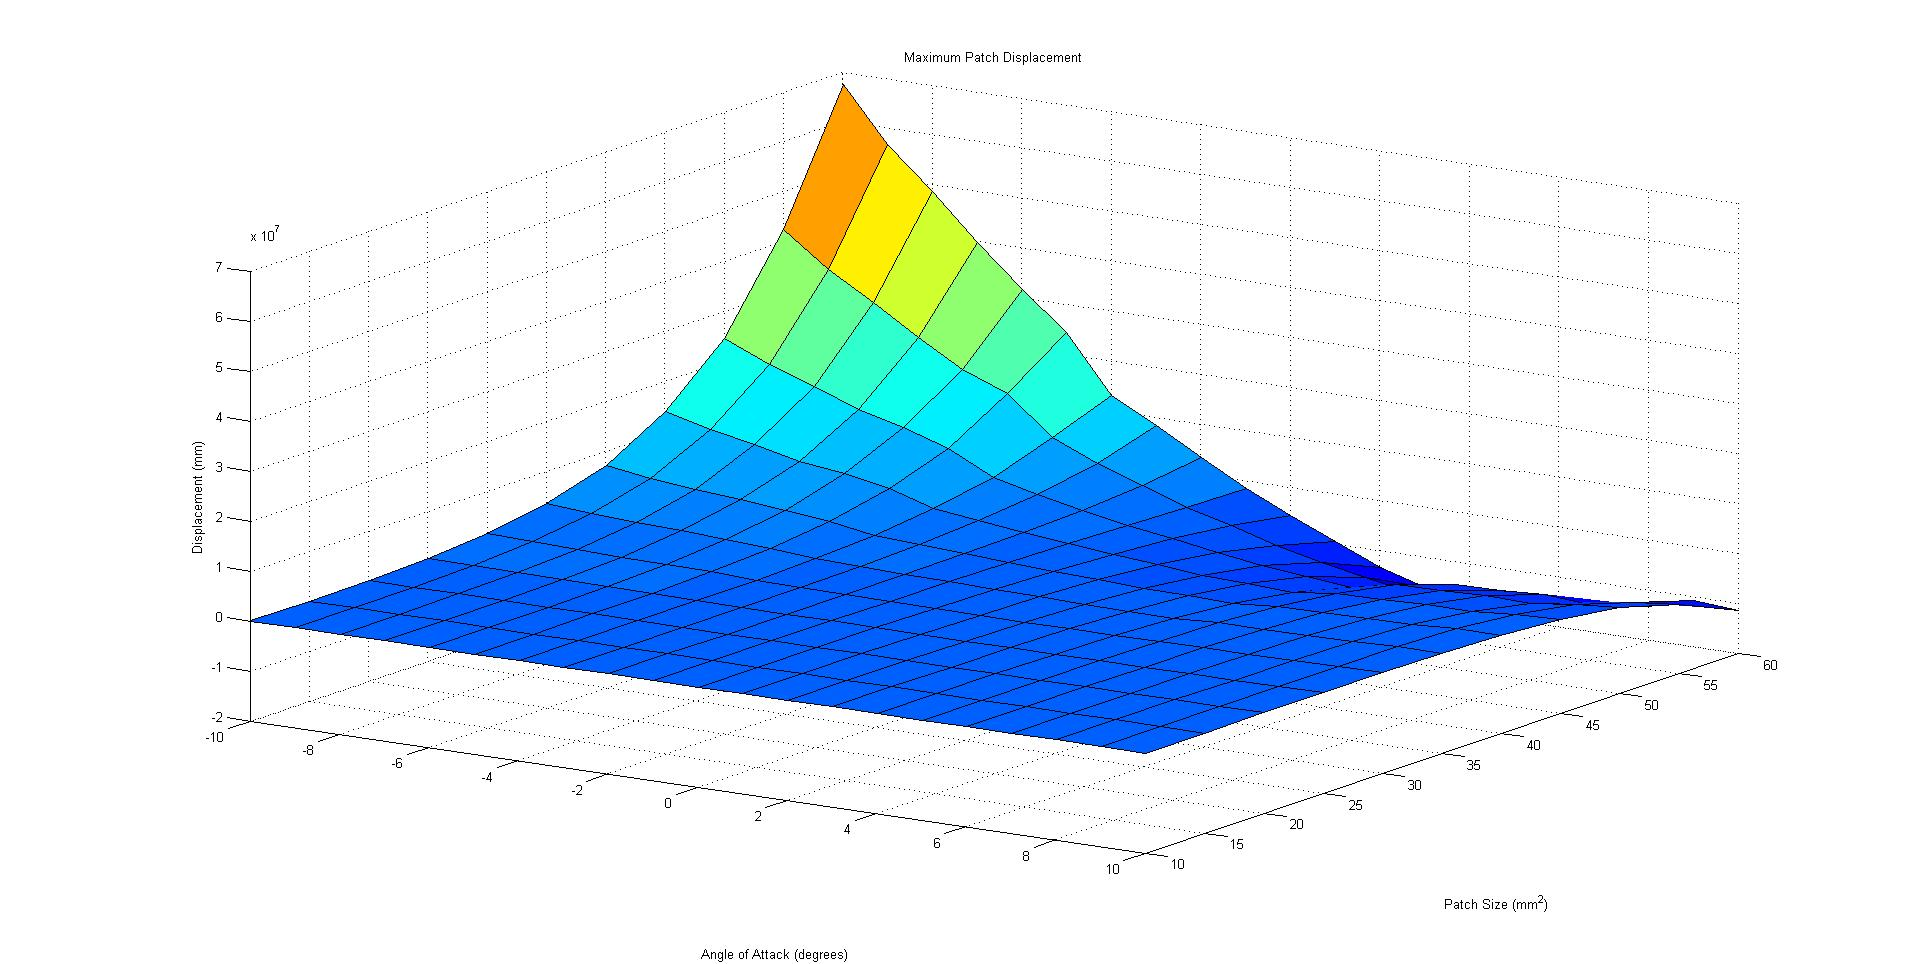
\includegraphics[width=1\linewidth]{Figures/MaximumPatchDisplacement.jpg}
\caption{The maximum displacement of an assumed thin plate with the average pressure applied from Figure\ref{fig:PProfile}}
\label{fig:PatchDisp}
\end{figure}

Now that the lattic pitch size has been determined the rest of the wing design can proceed. The wing was designed and built by Benjamin Jennett details of the design can be found in \cite{jenett2016digital}. The basics of the wing design will be included here for completeness. Figure \ref{fig:intStruct} shows the internal structure of wing. The cellular structures internal to the wing are created out of seven unique pieces and are formed of two primary geometries a cubic octahedron (cuboct) and a rhombic dodecahedron, also known as kelvin lattice, where the cubocts make up the rigid center with the lattice pitch determined above. The kelvin lattice makes up the trailing edge and has twice the pitch lattice that the cuboct section does allowing for the twist capabilities. The material properties for the carbon fiber reinforced polymer that the wing components were made out of can be seen in Table \ref{tab:cfrpProps}.

\begin{figure}
\hfill
\subfigure[Side View]{\includegraphics[width=7cm]{Figures/IMG_7232.JPG}}
\hfill
\subfigure[Tri-Iso View]{\includegraphics[width=7cm]{Figures/IMG_7233.JPG}}
\hfill
\caption{The internal structure of the wing is made from seven unique quasi isotropic carbon fiber components that were reversibly assembled as show in (a) and (b)}
\label{fig:intStruct}
\end{figure}

\begin{table}[h]
\begin{center}
\caption{Carbon Fiber Reinforced Polymer Properties}
\label{tab:cfrpProps}
\begin{tabular}{  p{4cm} p{5cm}}
Parameter&Value\\\hline
Layup Orientation&$0,45,90,0,-45,-90,-45,0^{o}$\\
Sheet thickness&$0.600''+/-0.005''$\\
Density&$1600 kg/m^{3}$\\
Young's Modulus (E)&$25-28 Gpa$\\
\end{tabular}
\end{center}
\end{table}

The active twist was achieved using a servo driven torque tube with a flexural arm to gain mechanical advantage an apply the appropriate amount of torque. The servo is mounted internally to the fuselage and acts as a means of redistributing the weight of the aircraft, further details on the actuation mechanism can be found in \cite{jenett2016digital}.

\section{Polystyrene Hollow Core Wing Design}

\begin{figure}[thpb]
\centering
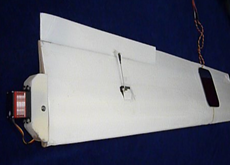
\includegraphics[width=0.5\linewidth]{Figures/AuroraWing.png}
\caption{Twist capable and outfitted with an actuation system that enabled in-flight active twist demonstration}
\label{fig:Awing}
\end{figure}

Our collaborators at Aurora Flight Sciences designed and built the wing in Figure \ref{fig:Awing} using fast construction methods, in particular a thermoplastic layer over a polystyrene hollow core wing. With the design constraints associated with the manufacturing process it was decided that it was necessary to make a geometrically insensitive airfoil, which they tested using XFOIL. The geometrically insensitive air foil is important from an modeling preservative for active twist because twist induced warping requires more computation and provides another variation to consider. Knowing this we performed benchtop testing to confirm that the aerodynamic properties of the airfoil do not change with twist.

\begin{figure}[thpb]
\centering
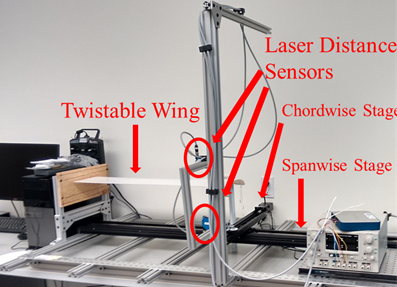
\includegraphics[width=0.75\linewidth]{Figures/AuroraWingBenchtopTest.png}
\caption{Airfoil measurement benchtop testing rig}
\label{fig:Atestrig}
\end{figure}

The benchtop testing to confirm the airfoil properties did not change with twist was done by scanning the cross section of the wing at various twist degrees and then using XFOIL to inspect the twist aerodynamic properties. The test rig used is show in Figure \ref{fig:Atestrig}. The laser distance sensors were placed on a C structure which was mounted on a linear stage to scan the chordwise directions while that was mounted on another stage to scan the spanwise direction. The scanning results can be seen in Figure \ref{fig:Ascan} and they show that there are minimal changes in the airfoil shape.

\begin{figure}[h]
\centering
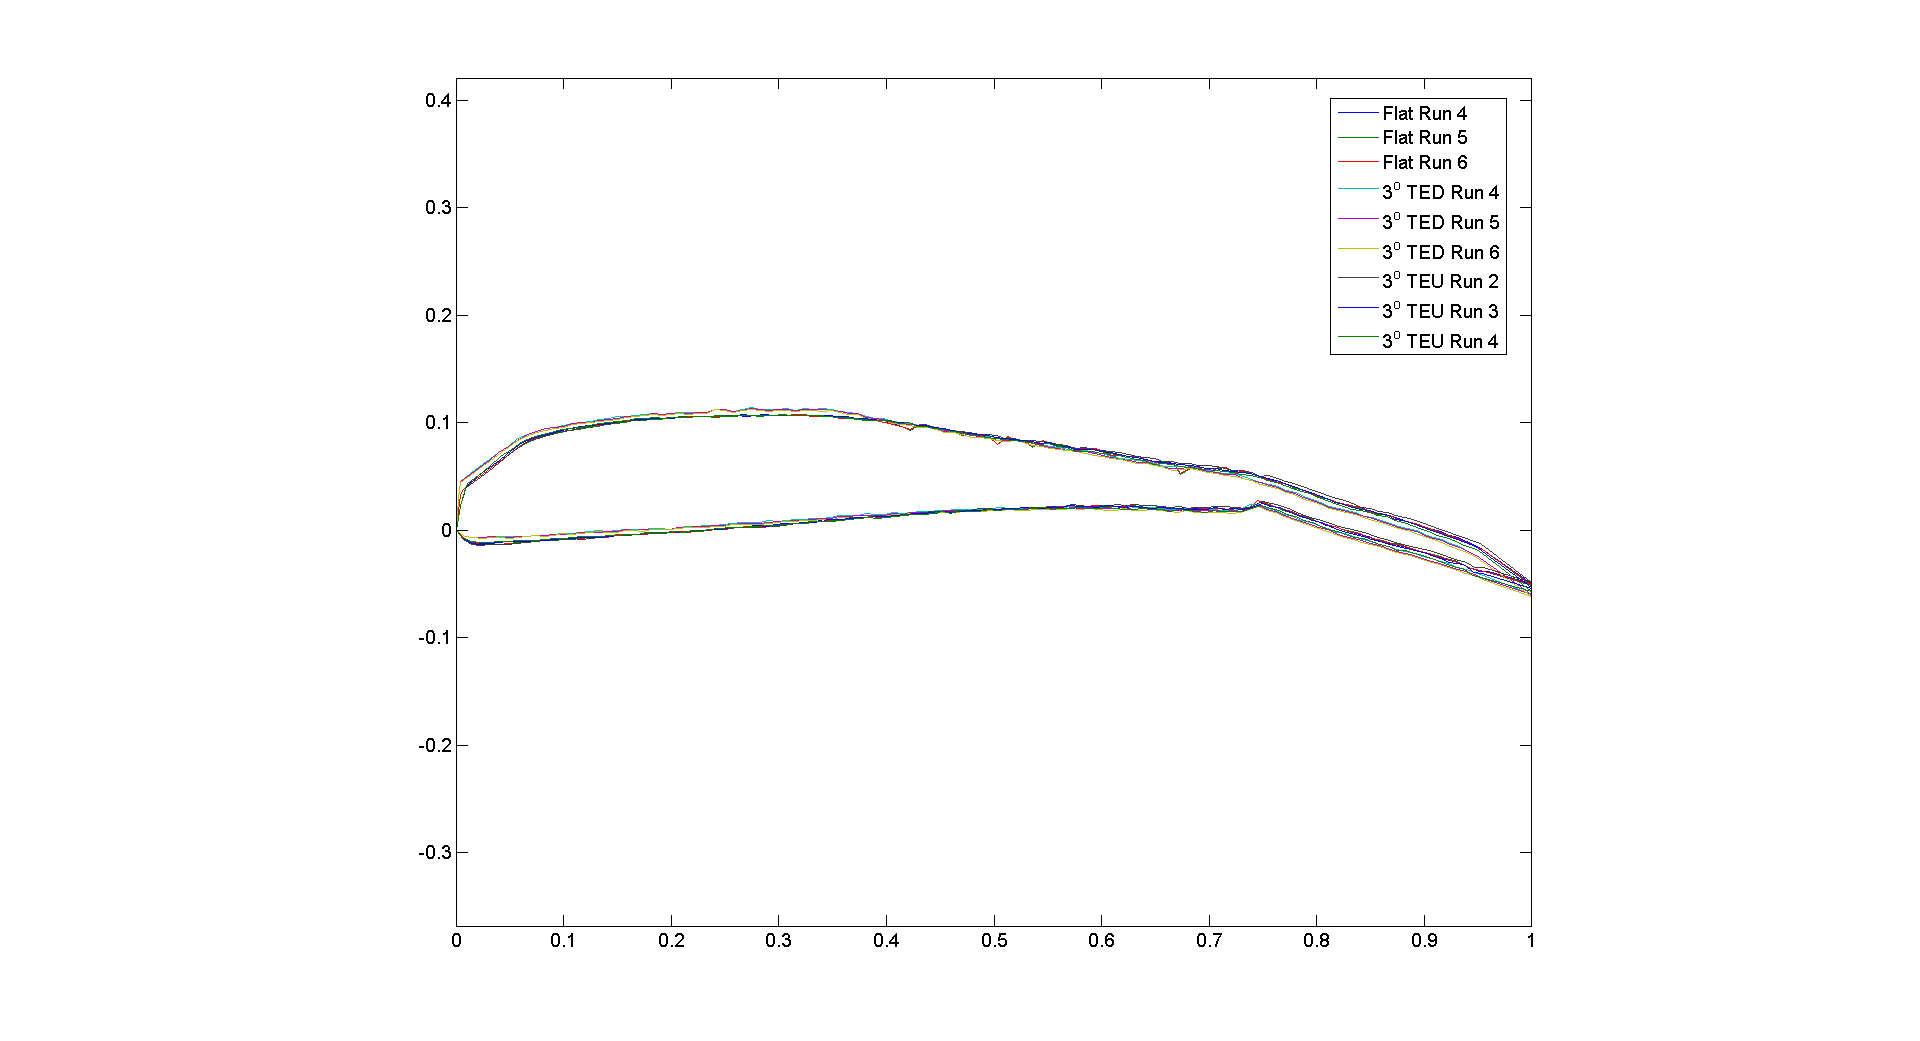
\includegraphics[width=0.75\linewidth]{Figures/AirfoilDirectMeasurements.png}
\caption{Comparison of airfoil profile for different amounts of twist}
\label{fig:Ascan}
\end{figure}

Figure \ref{fig:Alift} shows the lift profile for the measured airfoils, which are grouped fairly tightly. We chose to look at lift profiles for the first iteration of the test because the initial scans had some short comings. The configuration of the laser distance sensor was vertical in comparison to the stage which resulted in limited viewing capabilities of the nose. While we attempted to interpolate the rest of the nose location it was difficult due to the relatively few number of points. This had a disproportionate and unrealistic effect on the desired pitching coefficient when simulated in XFOIL; thus, we chose to use the lift as a baseline comparison. In future experiments, we will be using the laser distance sensors at an angle in order give and increased number of sample points around the nose.

\begin{figure}[thpb]
\centering
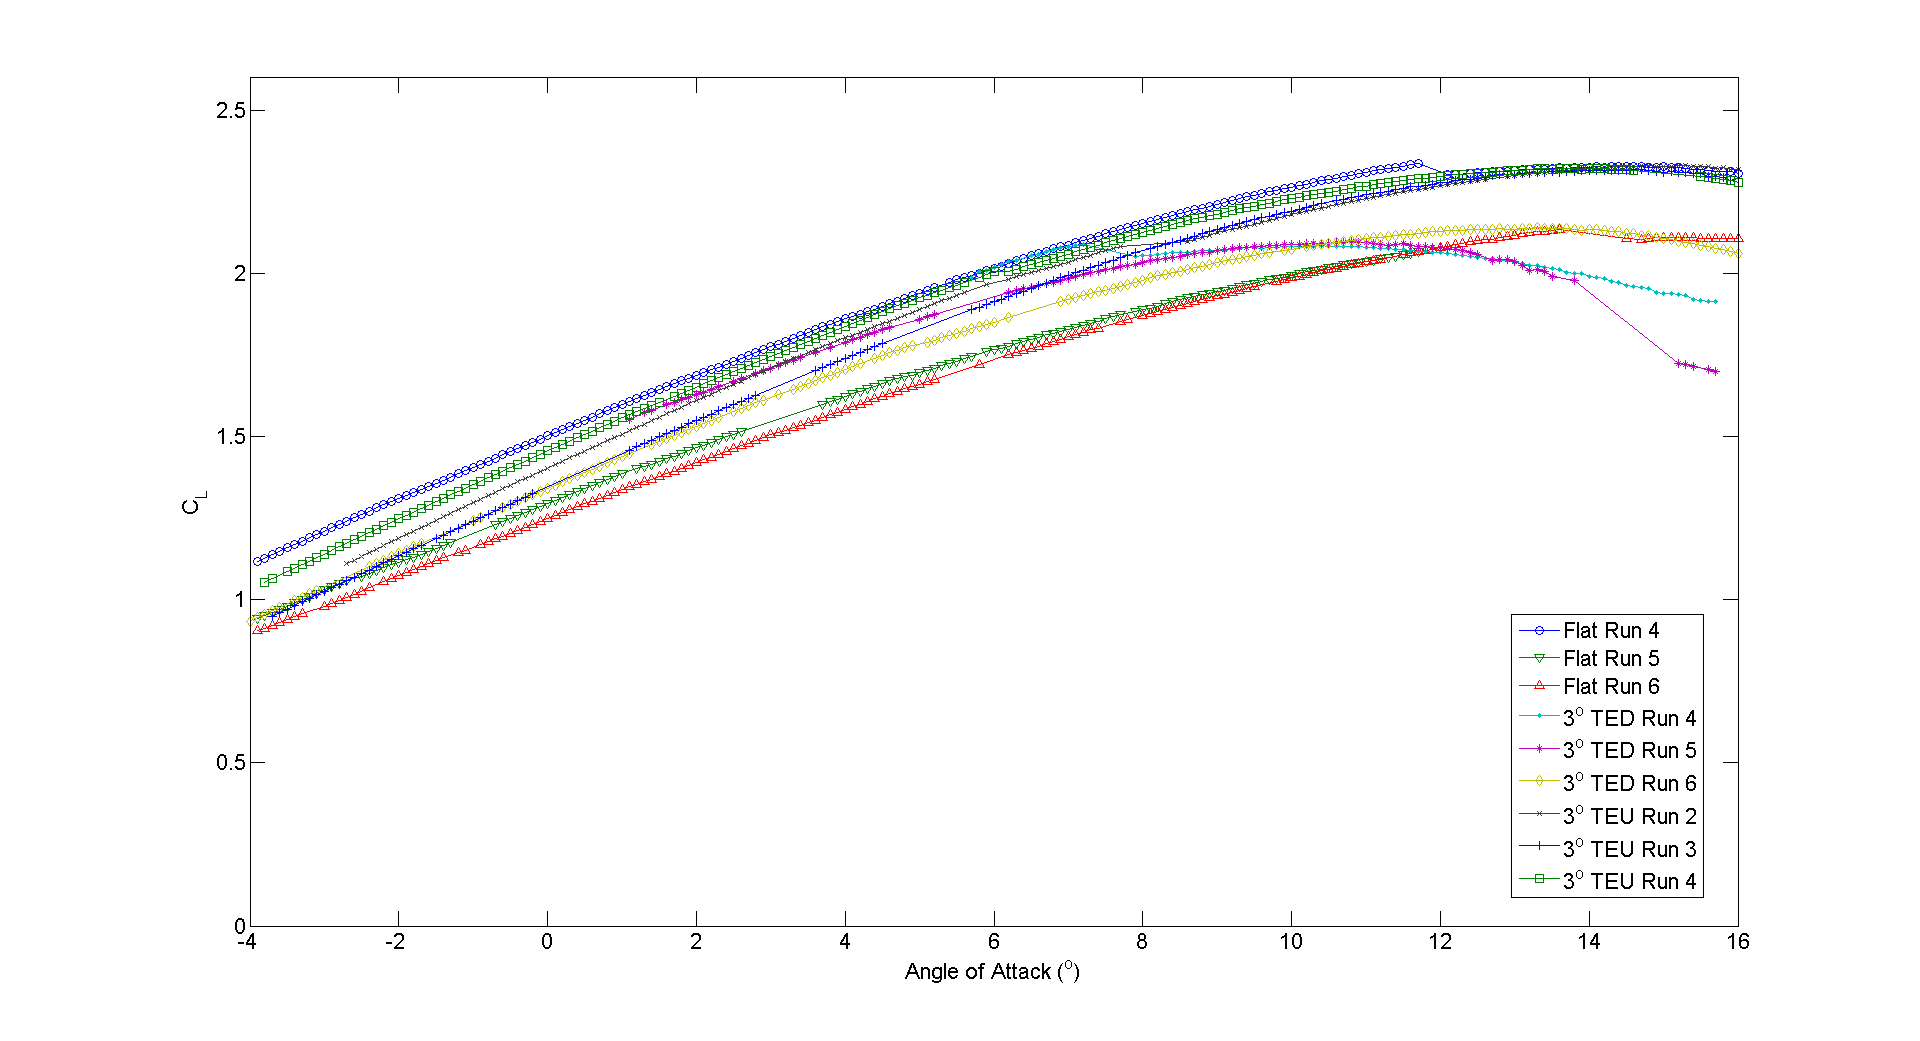
\includegraphics[width=0.75\linewidth]{Figures/CLDirectMeasurements.png}
\caption{XFOIL comparison of lift profile for measured airfoils}
\label{fig:Alift}
\end{figure}

With the completion of the design of the active twist wings it is important to test and validate the capabilities of the developed active twist wings.

%%%%%%%%%%%%%%%%%%%%%%%%%%%%%%%%%%%%%%%%%%%%%%%%%%%%%%%%%%%%%%%%%%%%%%%%%%%
\chapter{Testing and Validation}

The developed wings were testes and validated via bench-top testing as shown in the previous section but the composite lattice-based cellular structure active twist wing design was tested in a wind tunnel. The results from the wind tunnel testing were used to validate the performance and developed modeling technique.

\section{Wind Tunnel Testing}
The wind tunnel testing was performed at the NASA Langely 12-Foot Atmospheric, closed throat, annular return wind tunnel a graphic of the wind tunnel and its relevant parameters can be seen in Figure \ref{fig:windTunnel}. Figure \ref{fig:flex} shows the active twist aircraft mounted in the wind tunnel.

\begin{figure}[thpb]
\centering
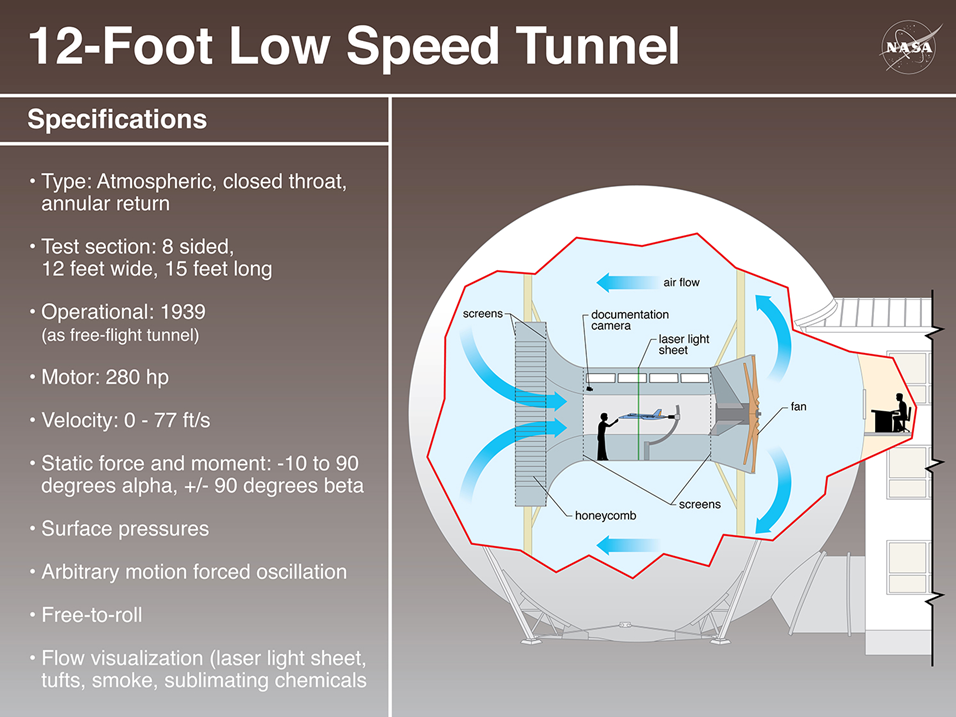
\includegraphics[width=1\linewidth]{Figures/12FootWindTunnel.png}
\caption{Diagram of NASA 12-Foot Wind Tunnel with relevant facts}
\label{fig:windTunnel}
\end{figure}

\begin{figure}[thpb]
\centering
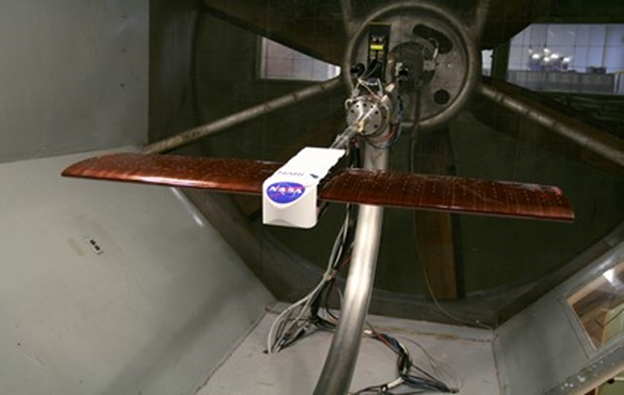
\includegraphics[width=0.75\linewidth]{Figures/wingFlex.png}
\caption{Active twist wing mounted in the wind tunnel}
\label{fig:flex}
\end{figure}

The methodology for wind tunnel testing was to assess the performance of the flexible design for a range of speed, angle of attack, and sideslip conditions with the wing twist angles deflected symmetrically and differentially. For comparison purposes, a similar matrix of conditions was tested using a rigid model with identical (neutral) outer model line geometry shown in Figure \ref{fig:rigid}. Flaperons were included on the rigid model to represent typical symmetric and differential control surfaces for comparisons to the flexible model undergoing commanded twist deflections. The rigid model was 3D printed from polycarbonate using the Fused Deposition Modeling process since the tests were aimed at measuring the aerodynamic properties and the extra weight was not a concern. During the test campaign, two copies of the flexible structure were tested.

\begin{figure}[thpb]
\centering
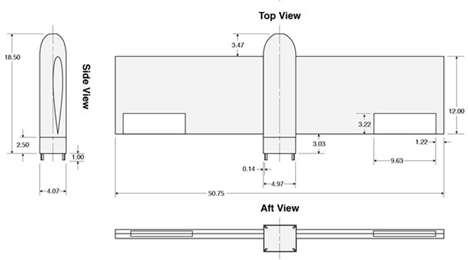
\includegraphics[width=0.75\linewidth]{Figures/rigidModel.png}
\caption{Design parameters for rigid model. The outer mold lines in the flat actuator trim condition are identical for the control and active twist models. Displayed dimensions are in inches.}
\label{fig:rigid}
\end{figure}

\section{Results and Validation}
The wind tunnel testing was broken into two parts the static test and the dynamic test. I define static tests as wind tunnel test where neither the active wing twist or the model was subjected to forced oscillations. 
\subsection{Static Wind Tunnel Results}
During the static wind tunnel testing, many different configurations were tested. In this section we will cover the results for a range of angle of attack, angle of sideslip, dynamic pressure, and wing twist (or control surface) deflection. In each configuration and test we are also validating and comparing our simulations, all of the parameters for which can be found in Table \ref{tab:vlmConfig}

\begin{table}[h]
\begin{center}
\caption{Shape and material parameters for VLM simulation}
\label{tab:vlmConfig}
\begin{tabular}{  p{6cm} p{1.9cm}}
Parameter&Value\\\hline
Half Span&$0.5795m$\\
Wing Cord&$0.3048m$\\
Body Width&$0.126238m$\\
Body Cord&$0.3048m$\\
Number of Spanwise Wing Panels&$32$\\
Number of Spanwise Body Panels&$4$\\
Number of Cordwise Panels&$8$\\
Rotational Area Moment of Inertia&$3.8918e^{-05}m^4$\\
Cross Sectional Area&$0.0076m^2$\\
Shear Modulus&$.169 MPa$\\
Density&$0.01543\frac{kg}{m^3}$\\
\end{tabular}
\end{center}
\end{table}  

\subsubsection{Symmetric Twist}

The first experiments performed in the wind tunnel were symmetric static tests with varying angles of attack, followed by symmetric flaperon deflection angles (labeled “flap” in the graphics) or tip twist in the case of the flexible models. If we look at Figure \ref{fig:CL}, we can see that there is significant of overlap between the results for each model, as would be expected due to the overall geometric similarities. It can also be seen that the “$10^o$ Flap” curve (Figure \ref{fig:CL} a) is very close to the “$6^o$ TipTwist” curve (Figure \ref{fig:CL} b), suggesting that there is a proportionality between the control effectiveness of two models.

\begin{figure}[thpb]
\hfill
\subfigure[Rigid model]{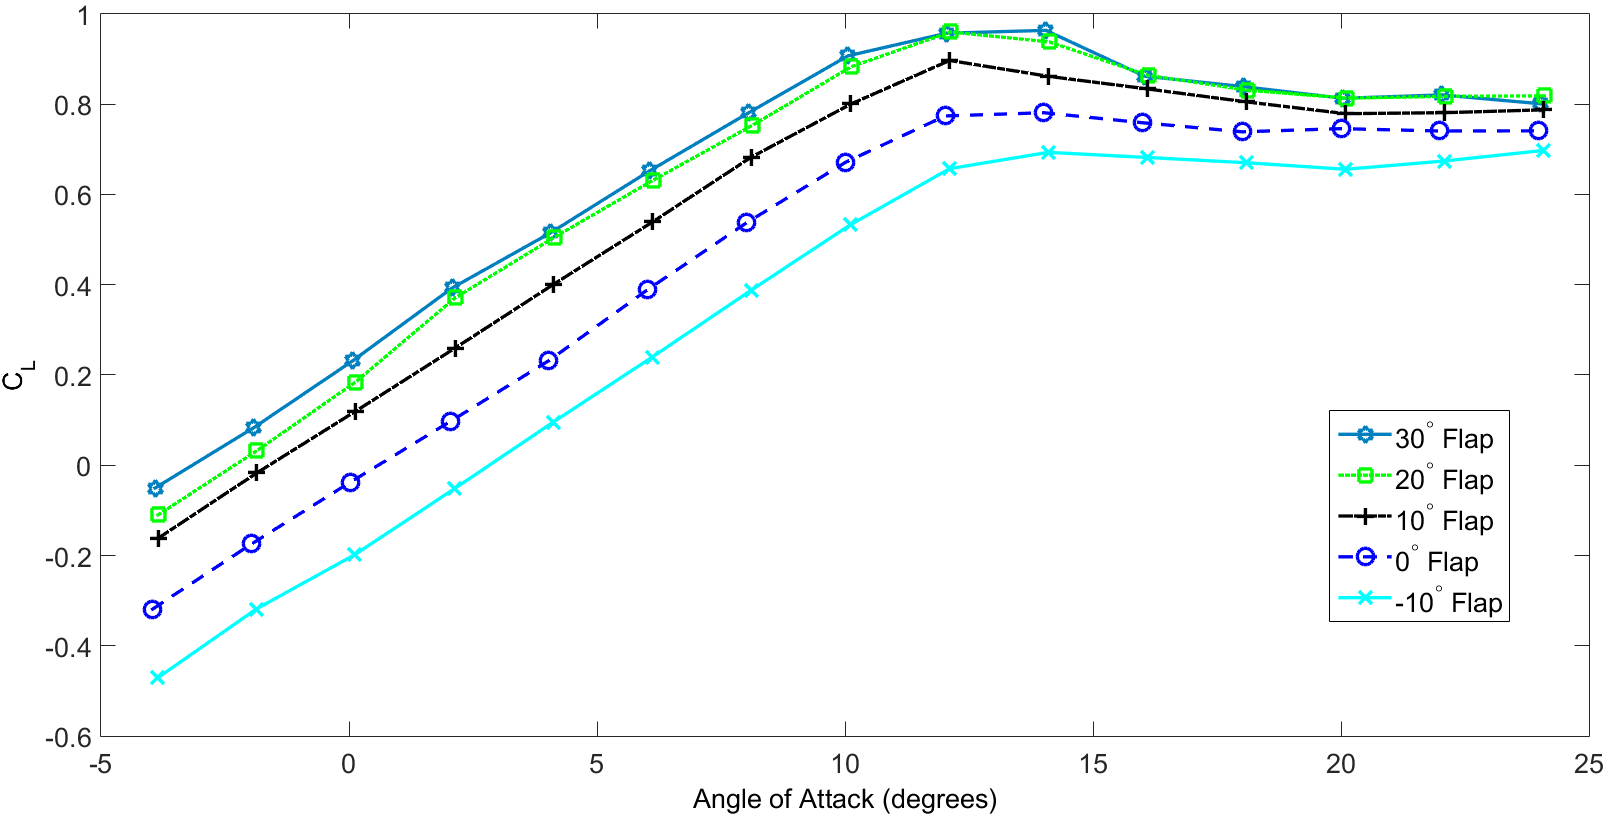
\includegraphics[width=7cm]{Figures/WindTunnelCLCompareRigid.png}}
\hfill
\subfigure[Flexible model]{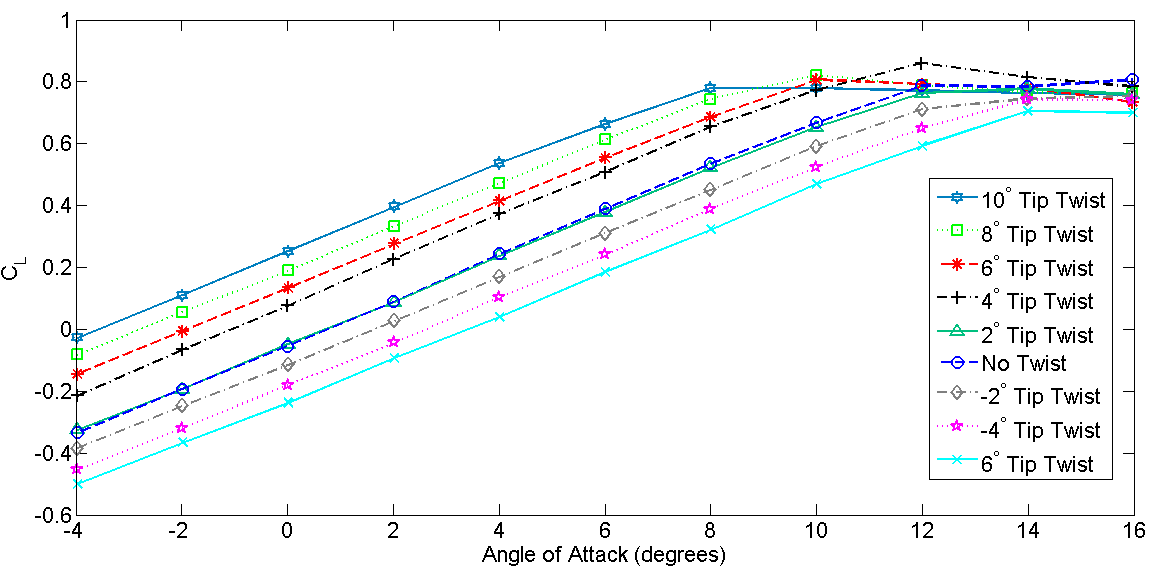
\includegraphics[width=7cm]{Figures/WindTunnelCLCompareFlex1.png}}
\hfill
\caption{Coefficient of lift curves}
\label{fig:CL}
\end{figure}

The similarity of the $6^o$ Tip Twist and 10o Flap results warrants closer inspection. Figure \ref{fig:6} compares the lift and drag curves for the two flexible models (labeled “Flex 1” and “Flex 2”), the rigid model, and the VLM simulation results of $6^o$ of tip twist. From Figure \ref{fig:6} we can see that all of the lift curves are very similar until the higher angles of attack, where the Flex 2 model has a little higher lift than the Flex 1, while the simulation predicts a little less. The biggest difference is in the drag curve, where at the lower angles of attack, the simulation agrees well with the wind tunnel results. However, the lack of accounting for the presence of the center body, and possibly viscous effects, cause the simulation results to diverge at an angle of attack of approximately two degrees. Prior to stall, the rigid model data also show a lower drag coefficient.  In the results that follow, no distinction is made between the results for Flex 1 and Flex 2, and are simply referred to as flexible model results.

\begin{figure}[thpb]
\hfill
\subfigure[Lift Curve]{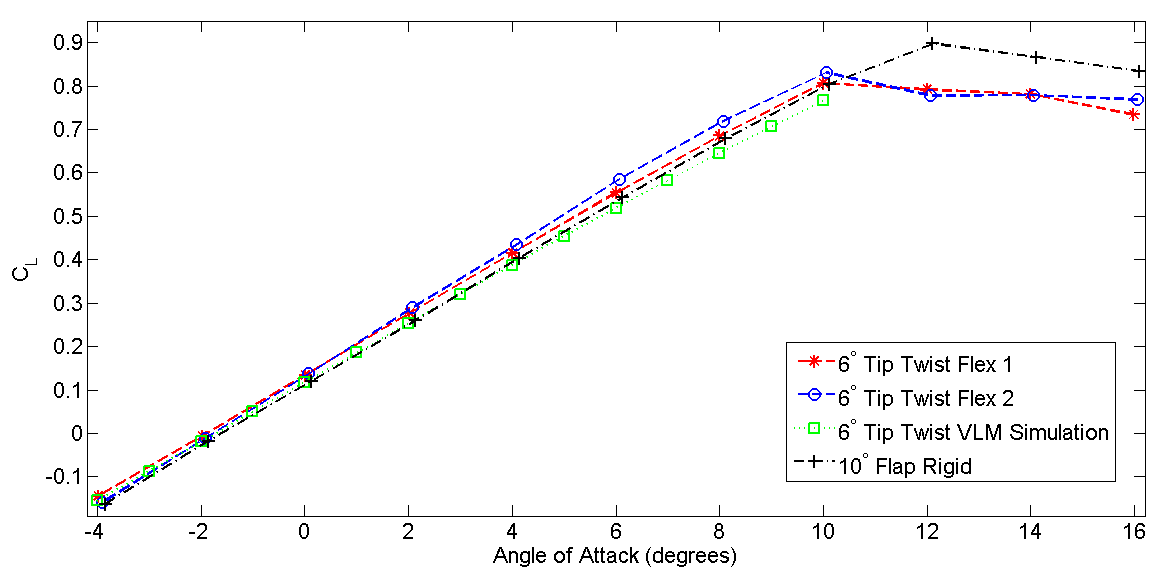
\includegraphics[width=7cm]{Figures/CLFlexSimandRigid.png}}
\hfill
\subfigure[Drag Curve]{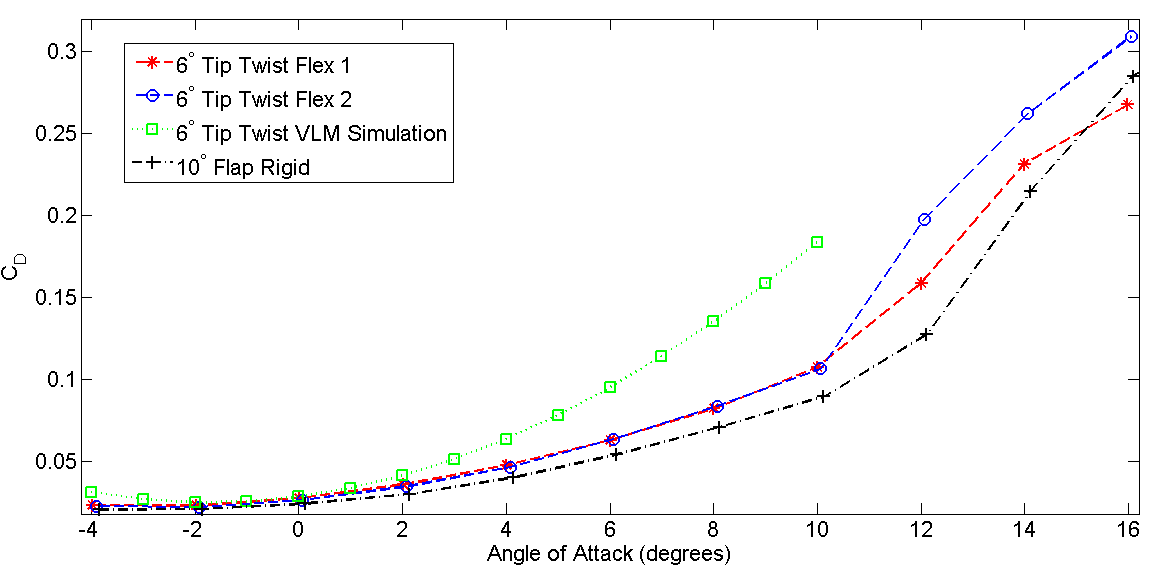
\includegraphics[width=7cm]{Figures/CDFlexSimandRigid.png}}
\hfill
\caption{Comparing the lift and drag curves of the rigid model, flexible models, and VLM simulations}
\label{fig:6}
\end{figure}

Figure \ref{fig:CD} shows the drag curves for the flexible and rigid model types. In general, the drag coefficient of the flexible model is higher at lower angles of attack.  For the equivalent control effectiveness, deflections of $10^o$ for the rigid model and $6^o$ for the flexible model, the drag data are very similar at the higher, yet pre-stall, angles of attack. 

\begin{figure}[thpb]
\hfill
\subfigure[Rigid model]{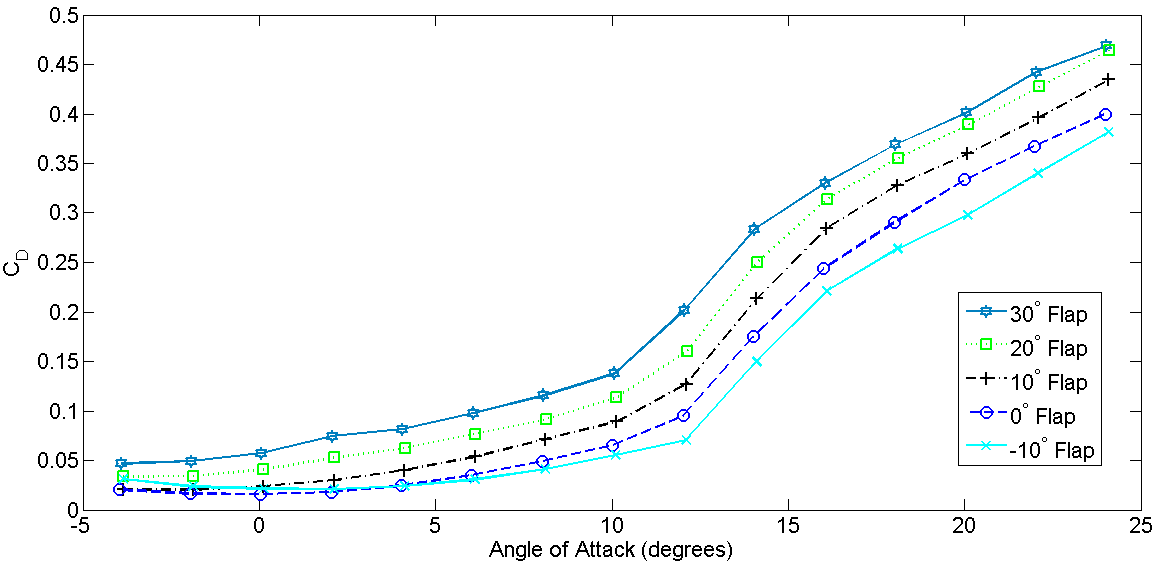
\includegraphics[width=7cm]{Figures/WindTunnelCDCompareRigid.png}}
\hfill
\subfigure[Flexible model]{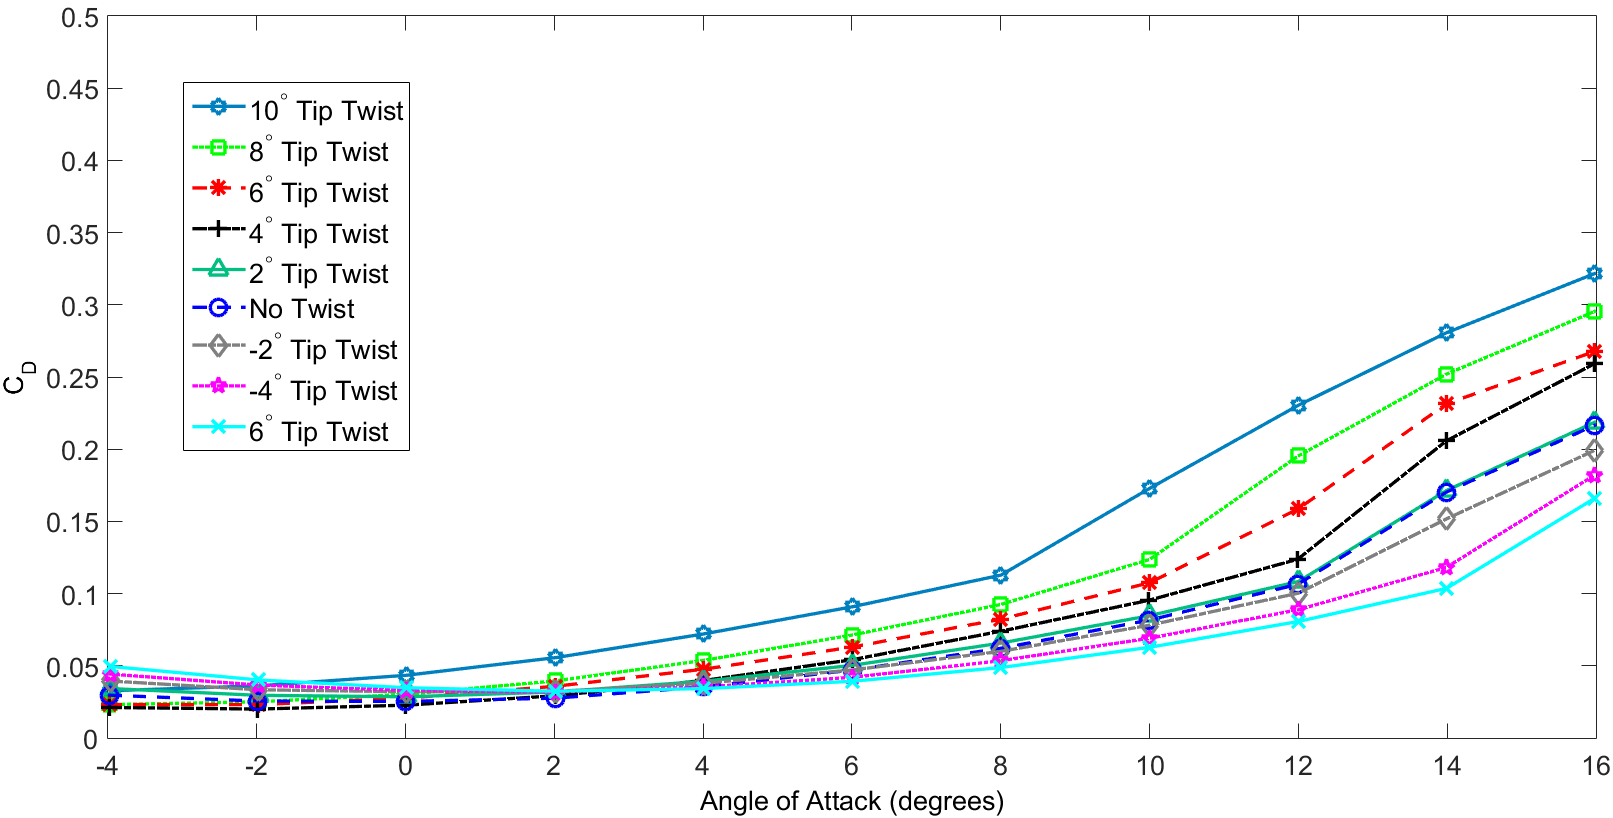
\includegraphics[width=7cm]{Figures/WindTunnelCDCompareFlex1.png}}
\hfill
\caption{Coefficient of drag curves}
\label{fig:CD}
\end{figure}

\begin{figure}[thpb]
\hfill
\subfigure[Rigid model]{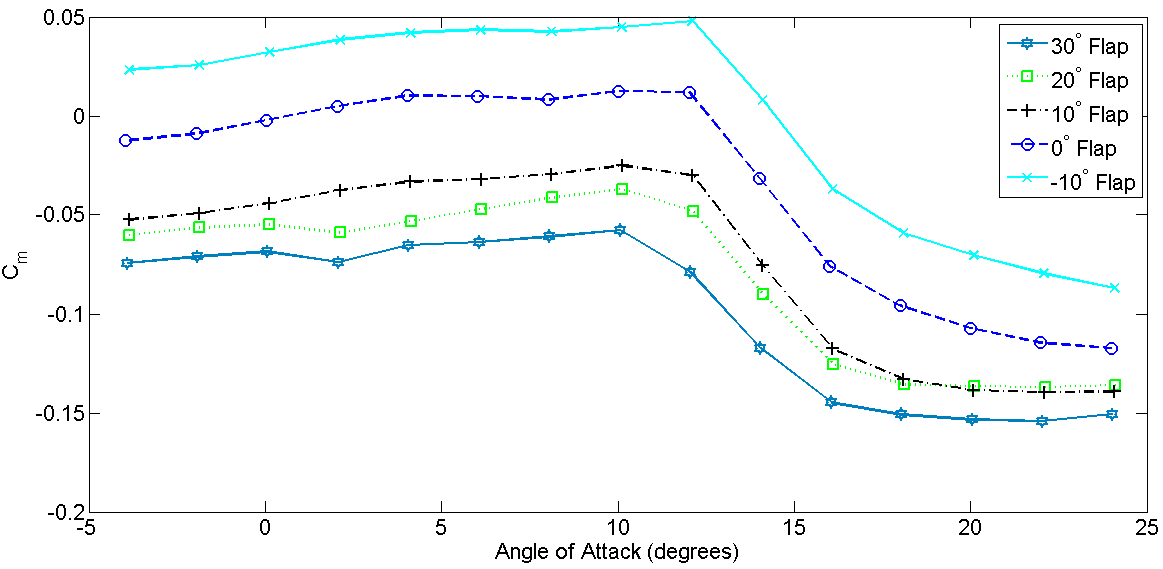
\includegraphics[width=7cm]{Figures/WindTunnelCmCompareRigid.png}}
\hfill
\subfigure[Flexible model]{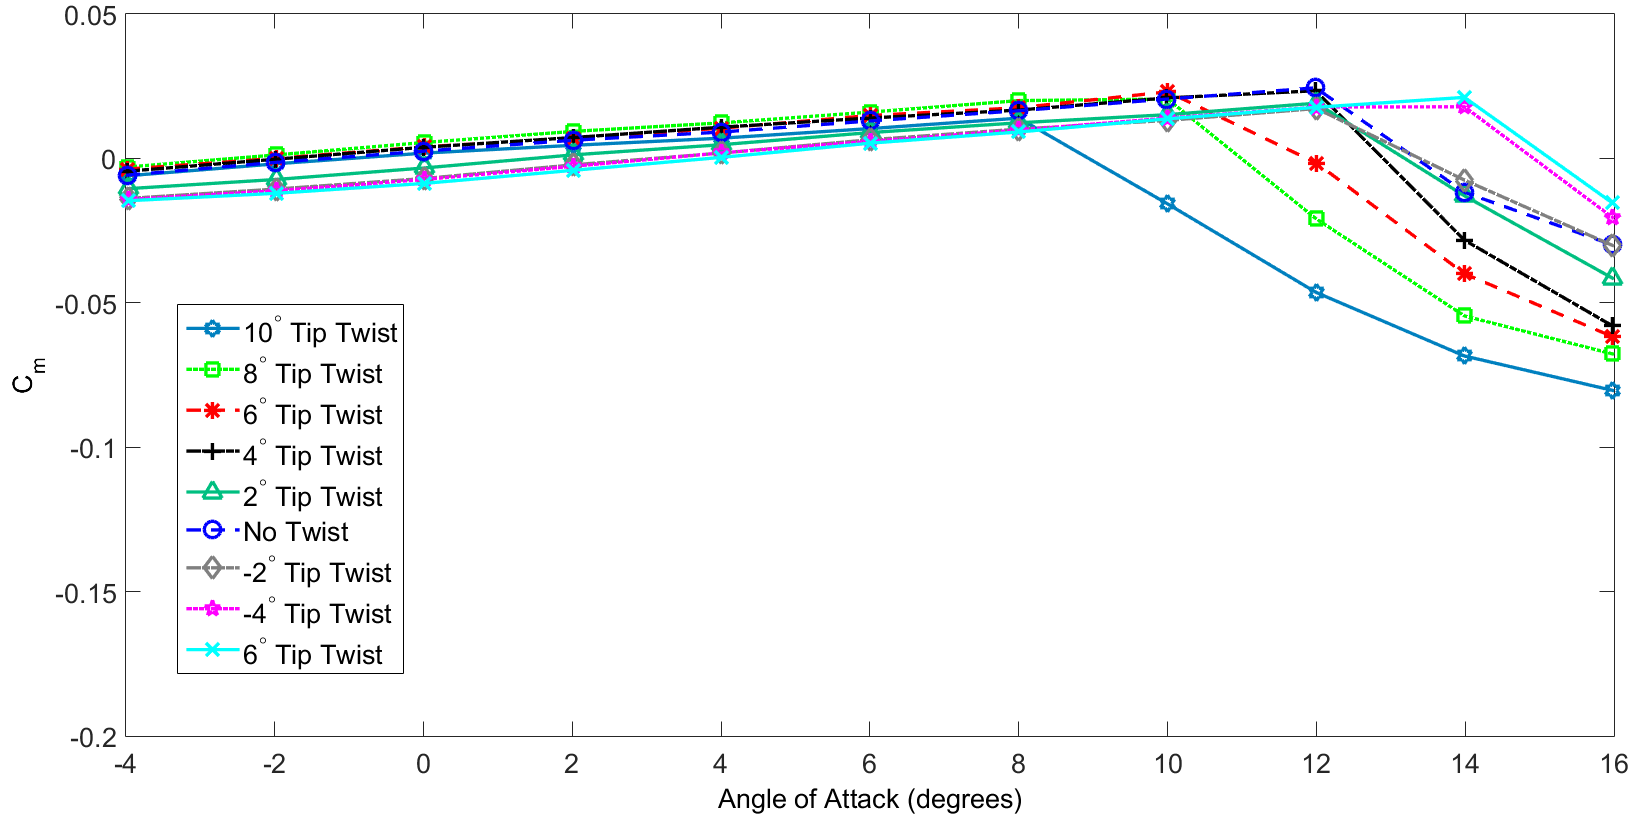
\includegraphics[width=7cm]{Figures/WindTunnelCmCompareFlex1.png}}
\hfill
\caption{Pitching moment coefficient curves}
\label{fig:CM}
\end{figure}

\begin{figure}[thpb]
\hfill
\subfigure[Rigid model]{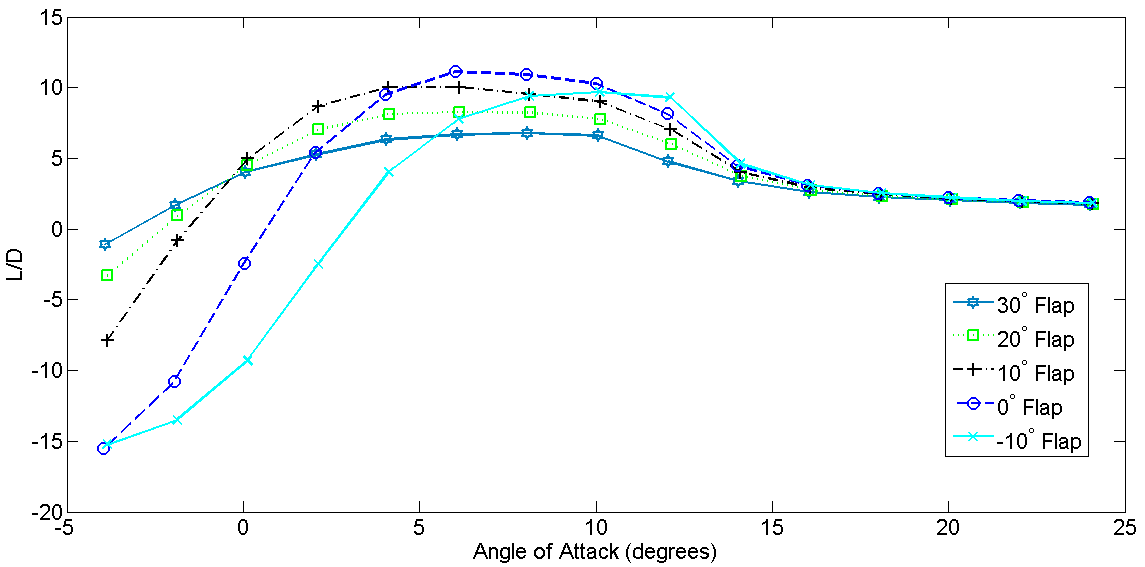
\includegraphics[width=7cm]{Figures/WindTunnelLDCompareRigid.png}}
\hfill
\subfigure[Flexible model]{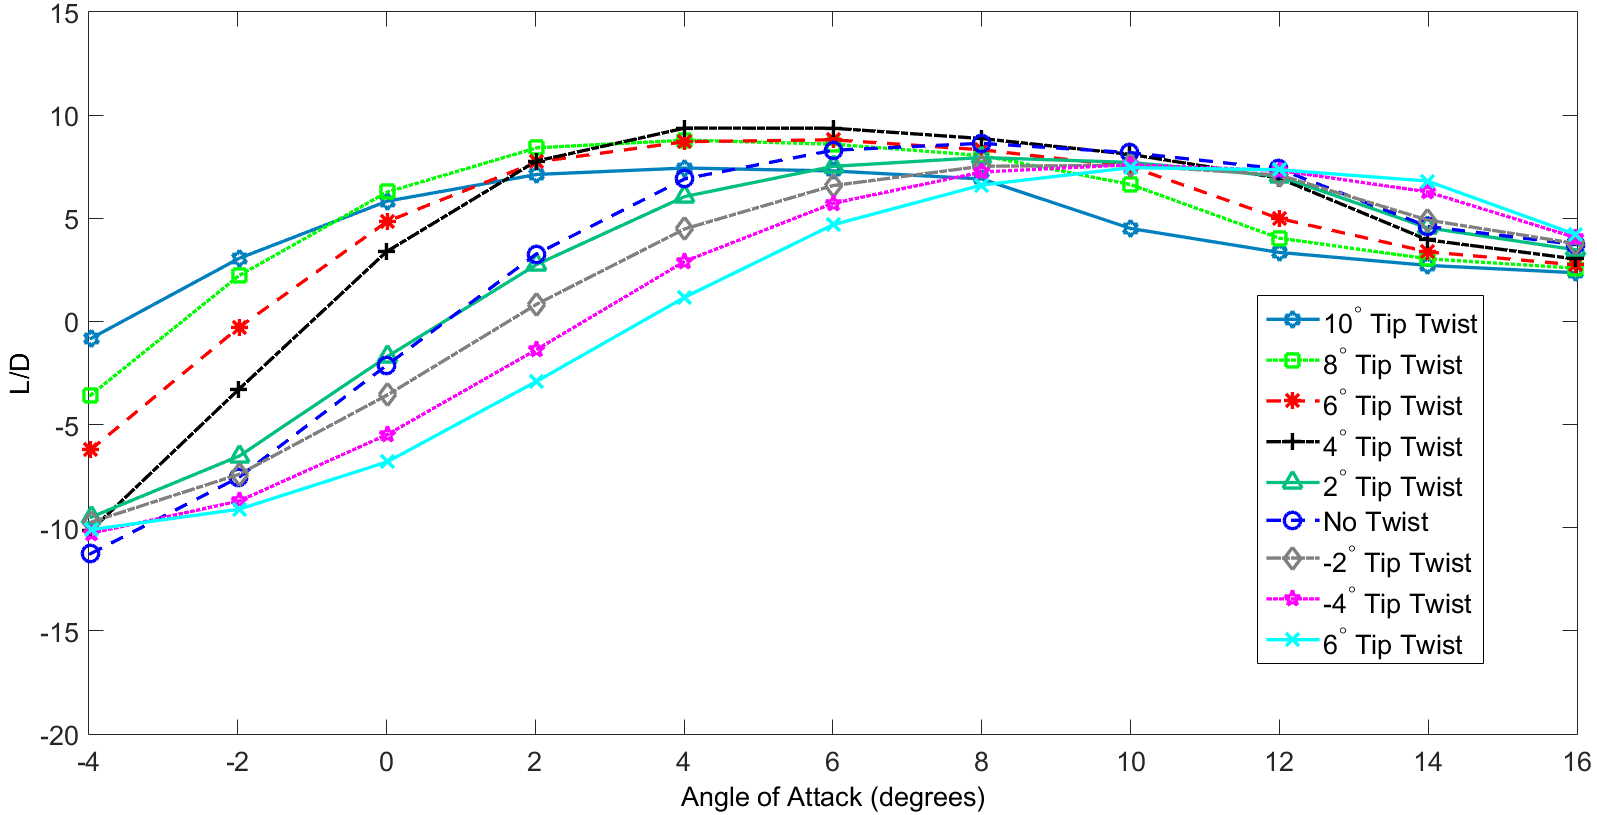
\includegraphics[width=7cm]{Figures/WindTunnelLDCompareFlex1.png}}
\hfill
\caption{Lift over Drag curves}
\label{fig:LD}
\end{figure}
Due to the configuration of the models (tailless, unswept flying wing without a reflexed camber line), it is not surprising to see Figure \ref{fig:CM} show that both models are unstable at low angles of attack. With no camber, a fuselage, and no tail, low or unstable static pitch stability is to be expected. Note that the flexible model is approaching marginal stability and the addition of a tail with minimal tail volume could easily make it stable. This also suggests that the design goal of mitigating the amount of airfoil warping was successful because the pitching moment coefficient is very similar to what we would expect for a symmetric airfoil.

One important part of the research was to determine the capabilities of the active twist system to improve efficiency over a large range of flight conditions. Figure \ref{fig:LD} shows the lift-over-drag curves for the rigid and flexible models. The maximum lift-to-drag ratio for the rigid model is slightly higher than that of the flexible models; however, the maximum lift-to-drag ratio for the rigid model comes solely from the $0^o$ Flap configuration. That is not the case for flexible model, where most of the tested configurations actually reach the maximum efficiency of the no-twist configuration, and some of them actually exceed it. In fact, the $4^o$ Tip Twist configuration has the highest lift-to-drag ratio for the flexible model. This suggests that for certain combinations of required lift and angle of attack, the flexible model would be more efficient than the rigid model and would be uniformly more efficient if the skins were comparable.

\subsubsection{Asymmetric Twist}
\begin{figure}[thpb]
\hfill
\subfigure[Rigid model]{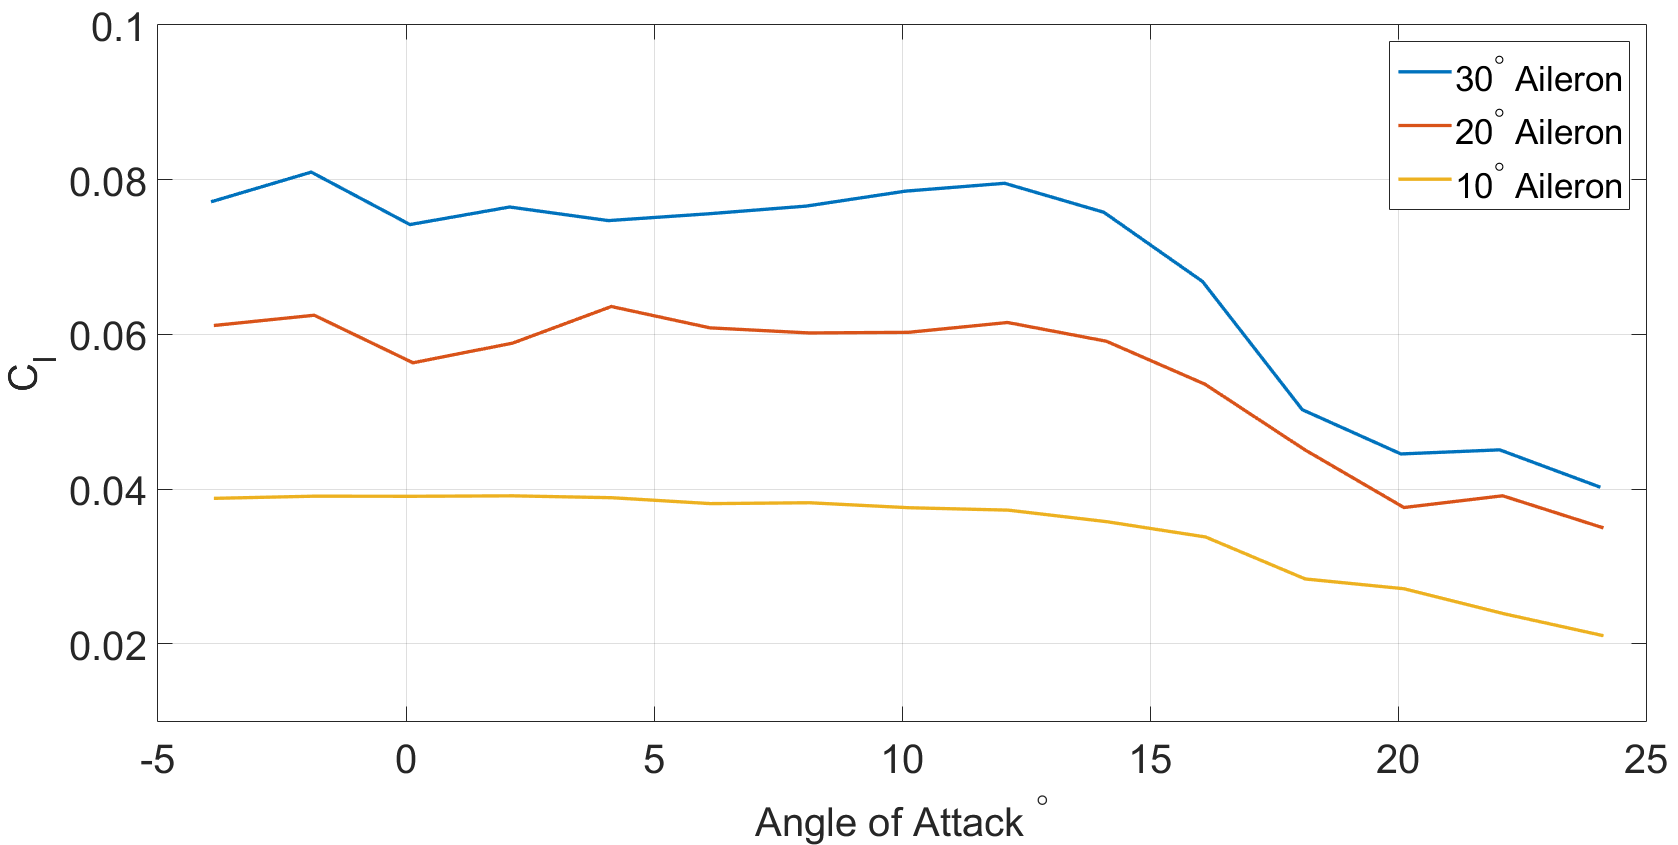
\includegraphics[width=7cm]{Figures/Q2RigidRoll.png}}
\hfill
\subfigure[Flexible model]{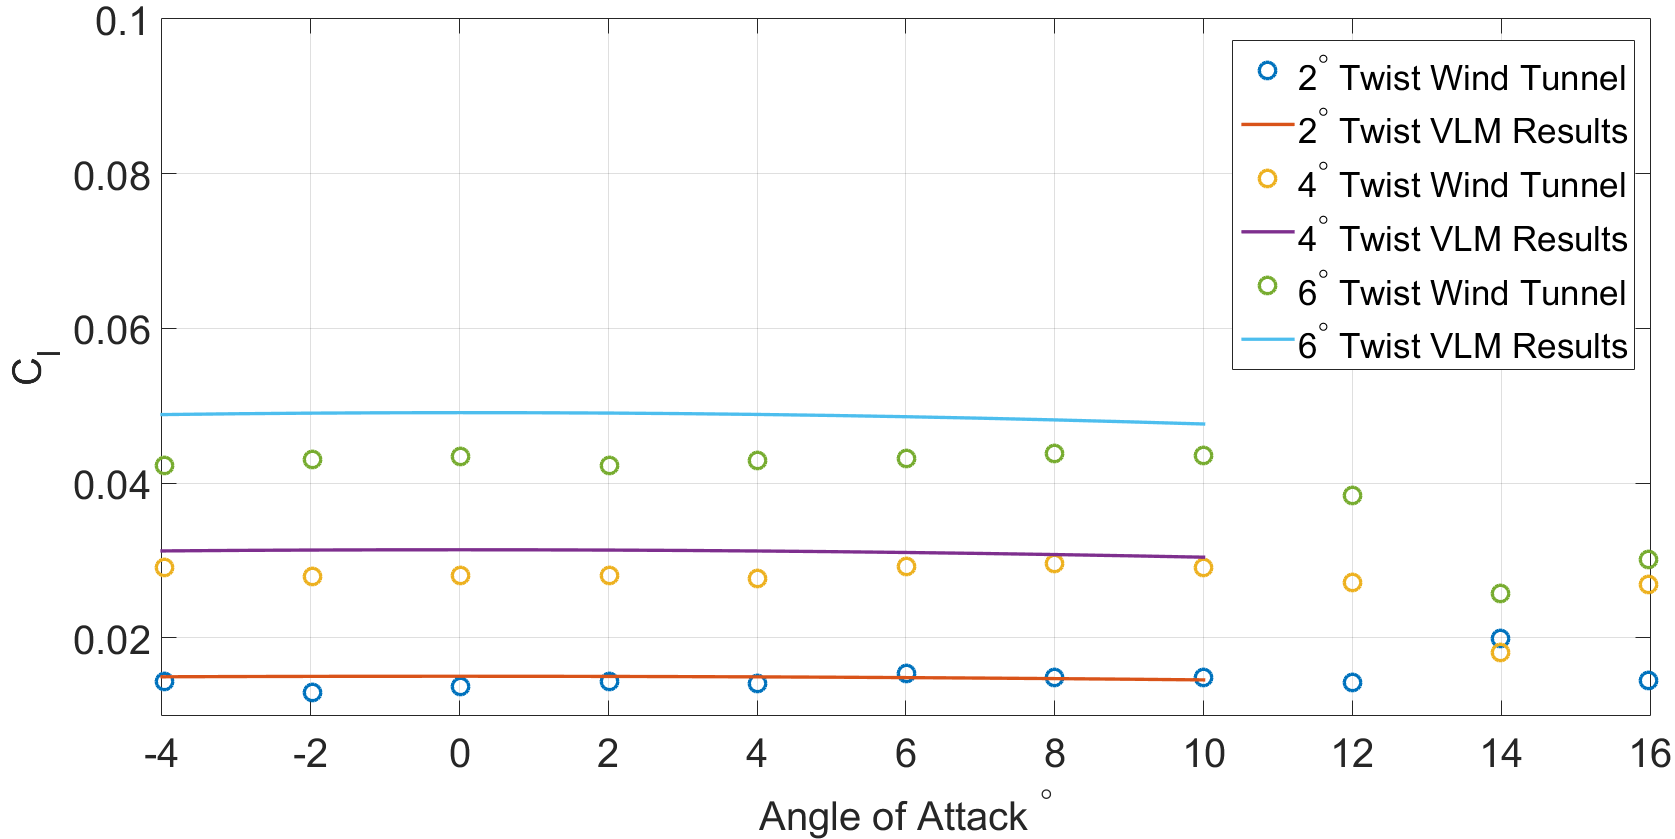
\includegraphics[width=7cm]{Figures/Q2Roll.png}}
\hfill
\caption{Roll characteristics at varying A) aileron angle (for rigid model) and B) wing tip twist angle (for flexible model and simulation model), as a function of angle of attack. (dynamic pressure = 2 psf)}
\label{fig:Q2Roll}
\end{figure}

In this section we will be focusing on the ability to generate roll and yaw moments. This is achieved primarily through asymmetric flaperon deflection (labeled aileron in the graphics) for the traditional rigid model and asymmetric twist for the flexible lattice model.

\begin{figure}[thpb]
\hfill
\subfigure[Rigid model]{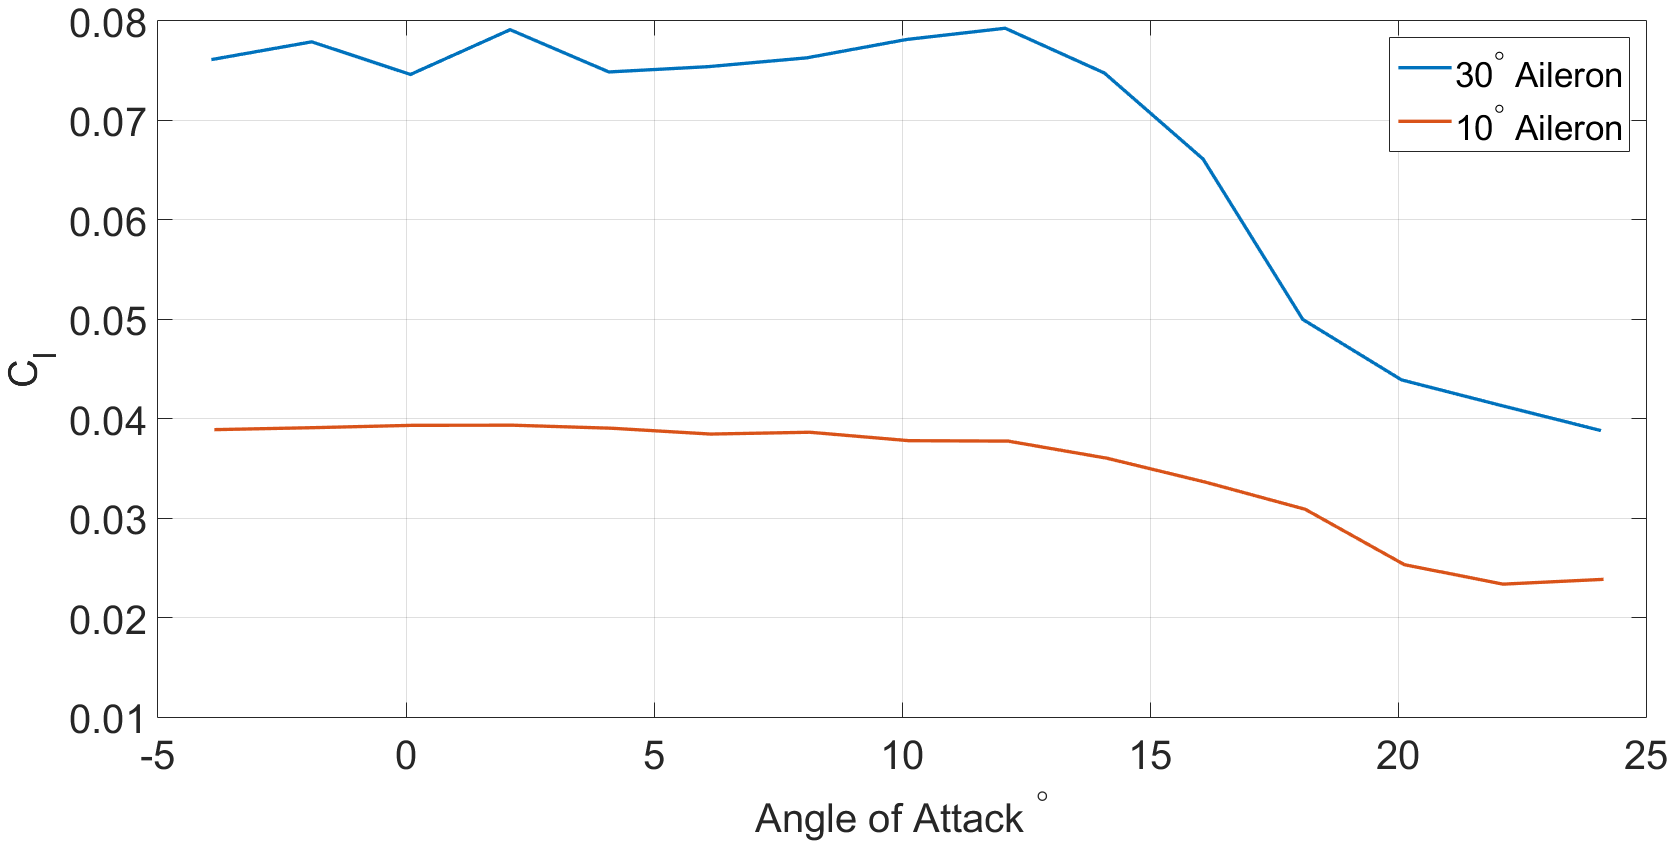
\includegraphics[width=7cm]{Figures/Q3RigidRoll.png}}
\hfill
\subfigure[Flexible model]{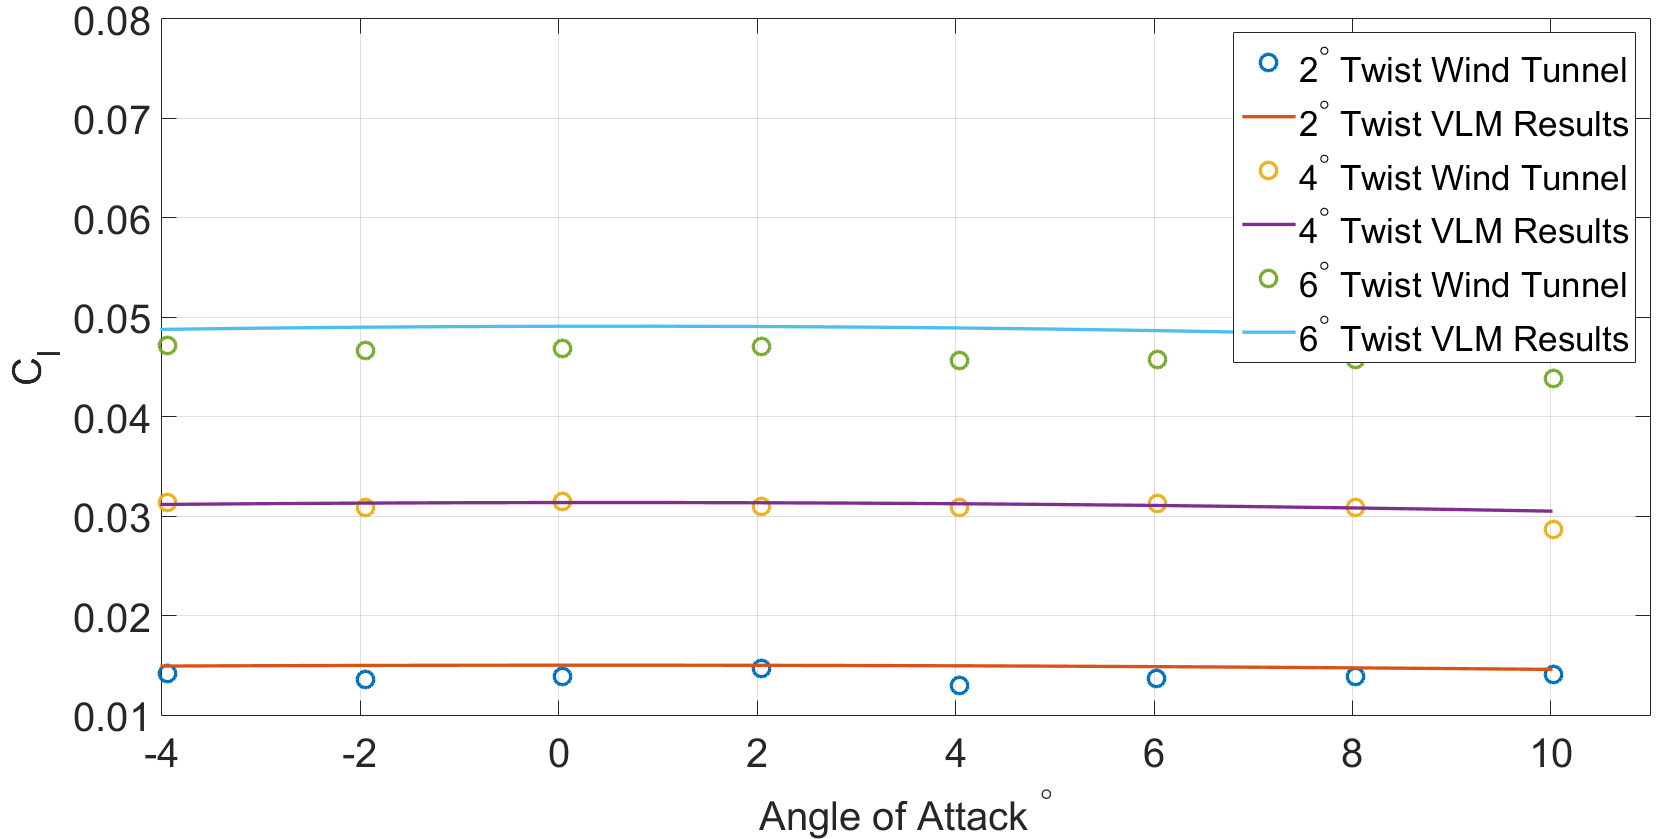
\includegraphics[width=7cm]{Figures/Q3Roll.png}}
\hfill
\caption{Roll characteristics at varying A) aileron angle (for rigid model) and B) wing tip twist angle (for flexible model and simulation model), as a function of angle of attack. (dynamic pressure = 3 psf)}
\label{fig:Q3Roll}
\end{figure}

The rigid model was tested at various dynamic pressures, from 2 psf to 4 psf, with a sweep of the angle of attack from $−4^o$ to $24^o$ and asymmetric flaperons at $10^o$, $20^o$, and $30^o$ deflected with the left device trailing edge down and the right device trailing edge up by the same deflection angle (equal and opposite – in a direction to nominally produce a right-wing-down rolling moment).  The flexible lattice wing model was tested over the same range of dynamic pressures but over a range of angle of attack from $−4^o$ to $16^o$ with asymmetric wing twist of $2^o$, $4^o$, and $6^o$ with two exceptions:  For the dynamic pressure of 3 psf there is no 4o wing twist; for the dynamic pressure of 4 psf the angle of attack only goes up to $10^o$.  The flexible-wing deflections were also equal and opposite in the same sense as described above.  At a dynamic pressure of 2 psf, Figure \ref{fig:Q2Roll} shows the incremental rolling moment coefficient of the rigid model and the flexible lattice wing model calculated by subtracting the neutral deflection data from the deflected cases. The various twist angles result in easily distinguishable rolling moment coefficients, ranging from approximately 0.015 to 0.045, and the simulation model compares reasonably well with the wind tunnel results, especially at the lower twist angles. Furthermore, the roll coefficient magnitude of the $6^o$ twist is comparable to the $10^o$ flaperon deflection case. This gives some proportionality to the amount of twist that would be needed to replicate the roll performance of flaperons.

\begin{figure}[thpb]
\hfill
\subfigure[Rigid model]{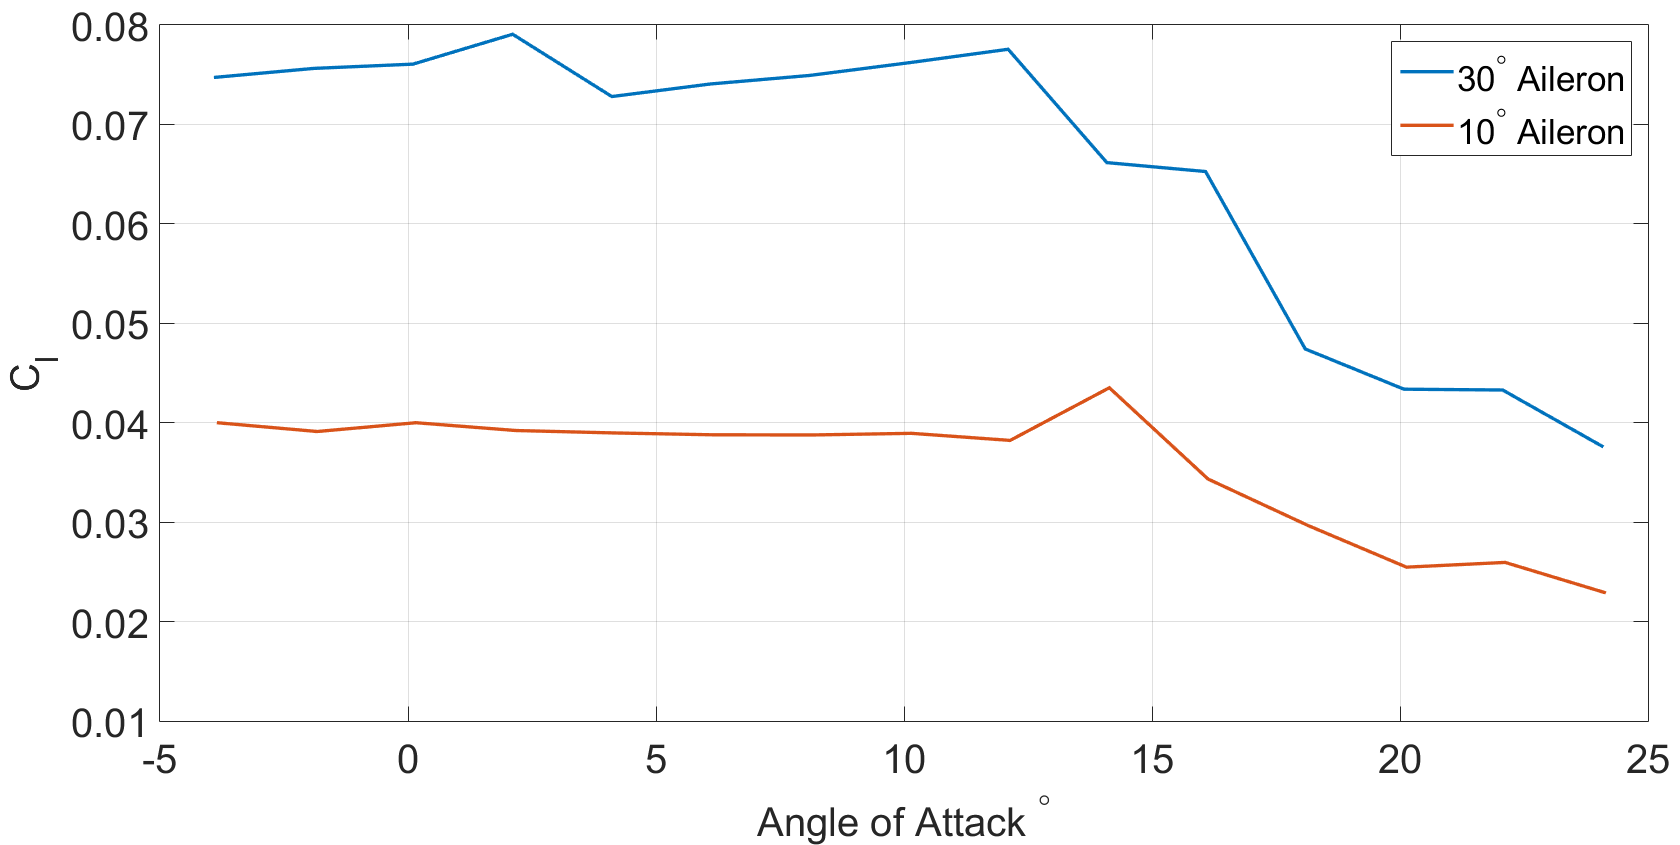
\includegraphics[width=7cm]{Figures/Q4RigidRoll.png}}
\hfill
\subfigure[Flexible model]{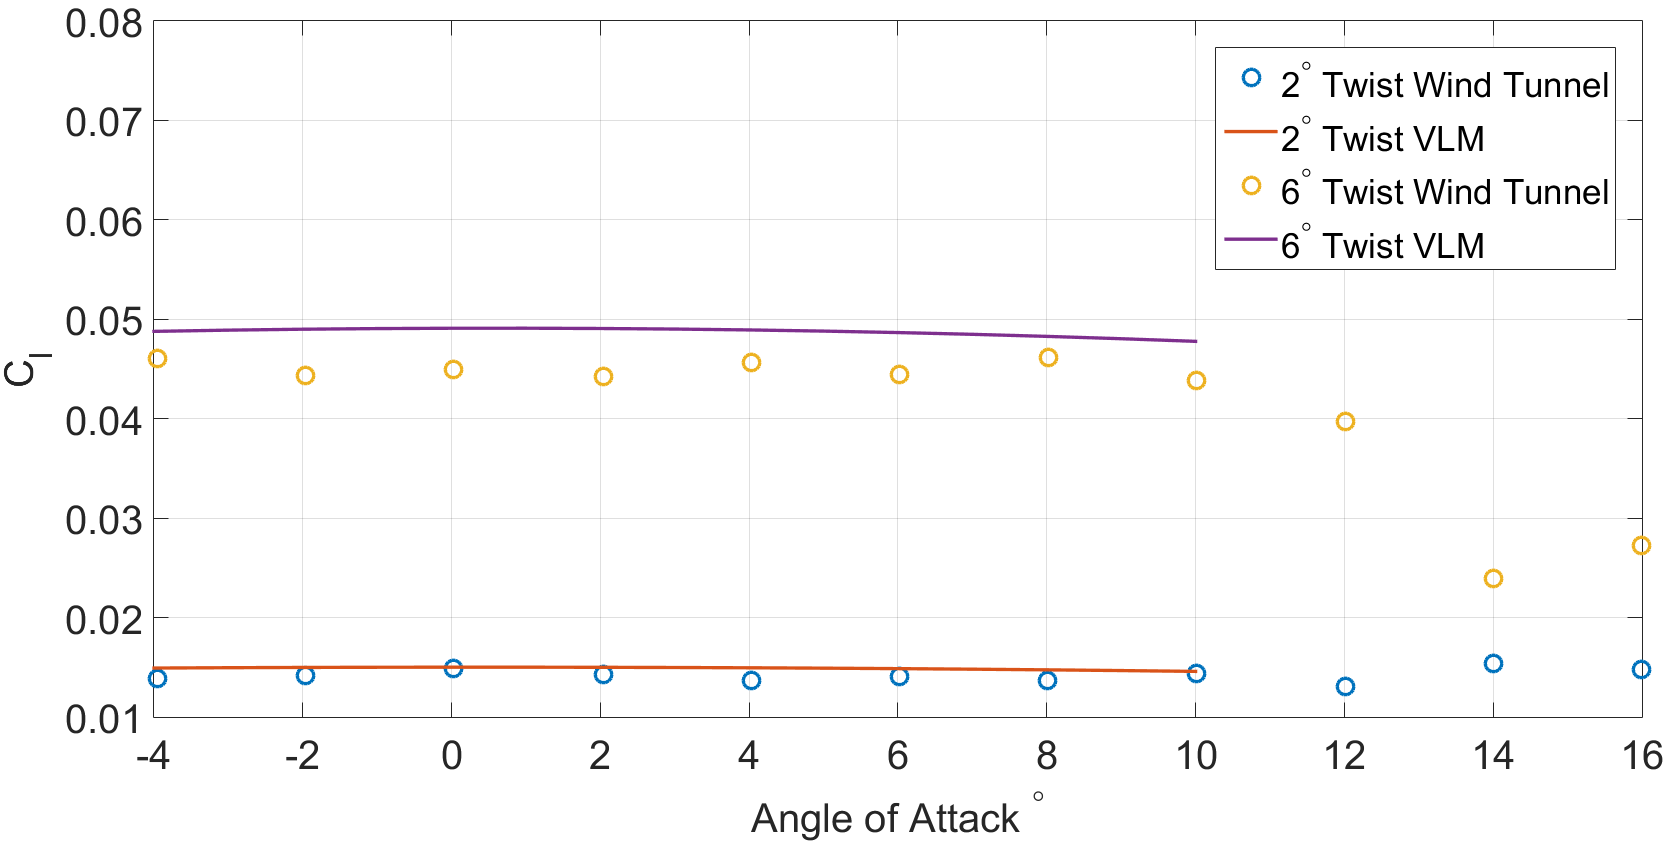
\includegraphics[width=7cm]{Figures/Q4Roll.png}}
\hfill
\caption{Roll characteristics at varying A) aileron angle (for rigid model) and B) wing tip twist angle (for flexible model and simulation model), as a function of angle of attack. (dynamic pressure = 4 psf)}
\label{fig:Q4Roll}
\end{figure}

Figures \ref{fig:Q2Roll}, \ref{fig:Q3Roll} and \ref{fig:Q4Roll} further indicate that the magnitude of the rolling moment coefficients for the rigid model does not change with increasing dynamic pressure, whereas for the flexible model, the roll magnitude continues to increase and begins to converge to the simulation results. We can expect that the simulation results will act as an effective upper bound for the performance of the flexible lattice wing. This is because the VLM method does not include the fuselage so the magnitude and the slope of the lifting line for a given wing is always optimistic which then is passed to the rolling cases when the twist is asymmetric. It is valuable to note that as the dynamic pressure increases the flexible lattice wing performs better. This means that at the same altitude but higher speeds the roll authority will be increased.

\begin{figure}[thpb]
\hfill
\subfigure[Rigid model]{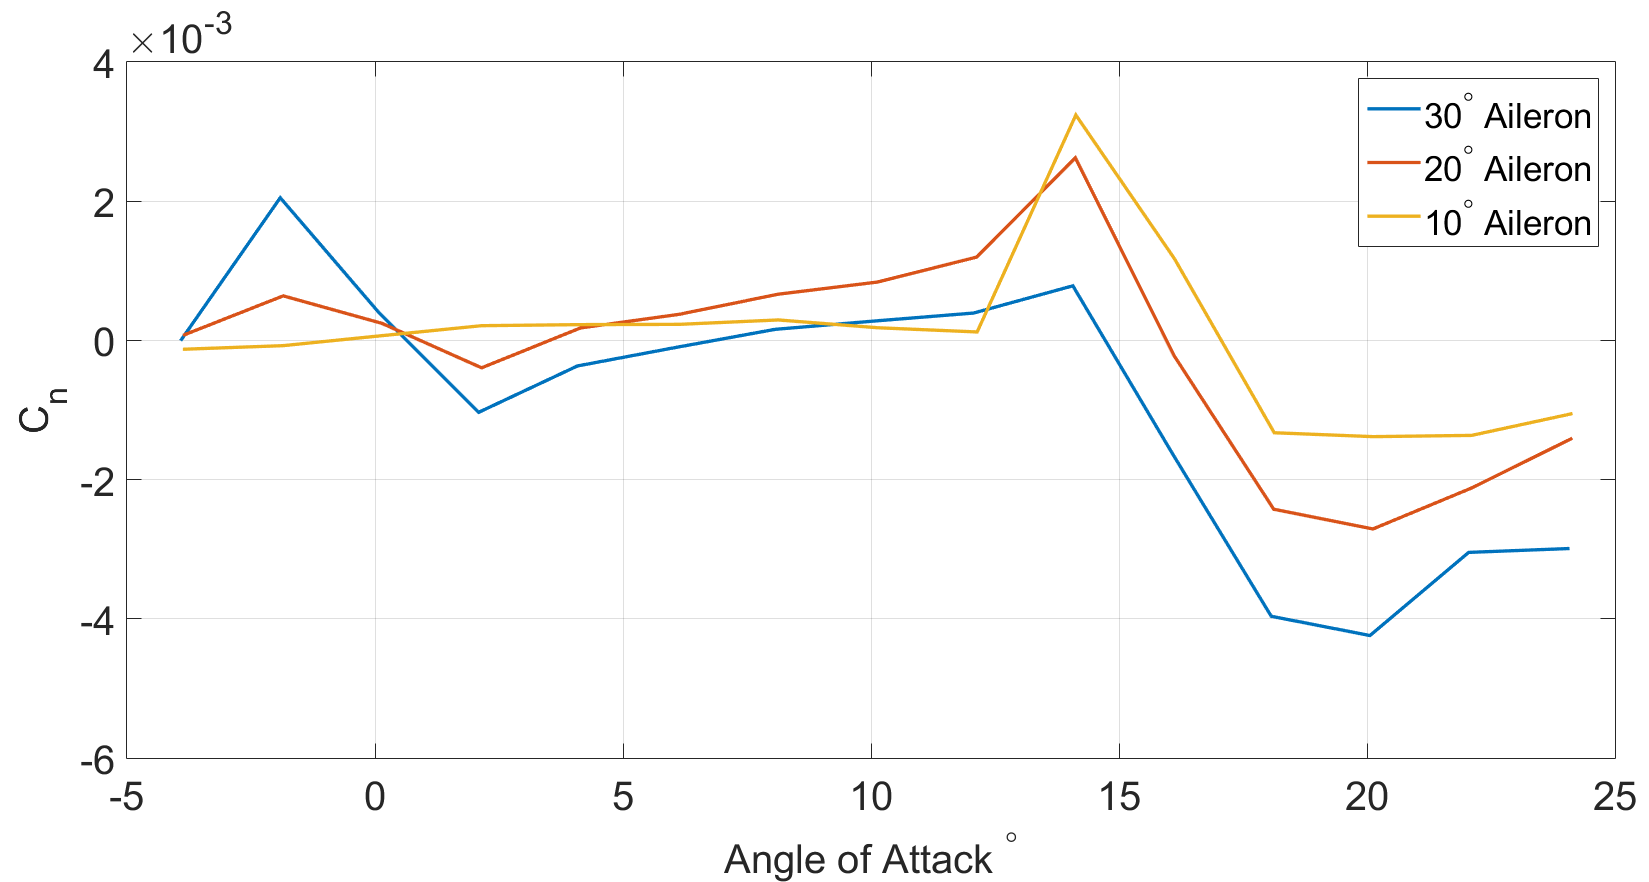
\includegraphics[width=7cm]{Figures/Q2RigidYaw.png}}
\hfill
\subfigure[Flexible model]{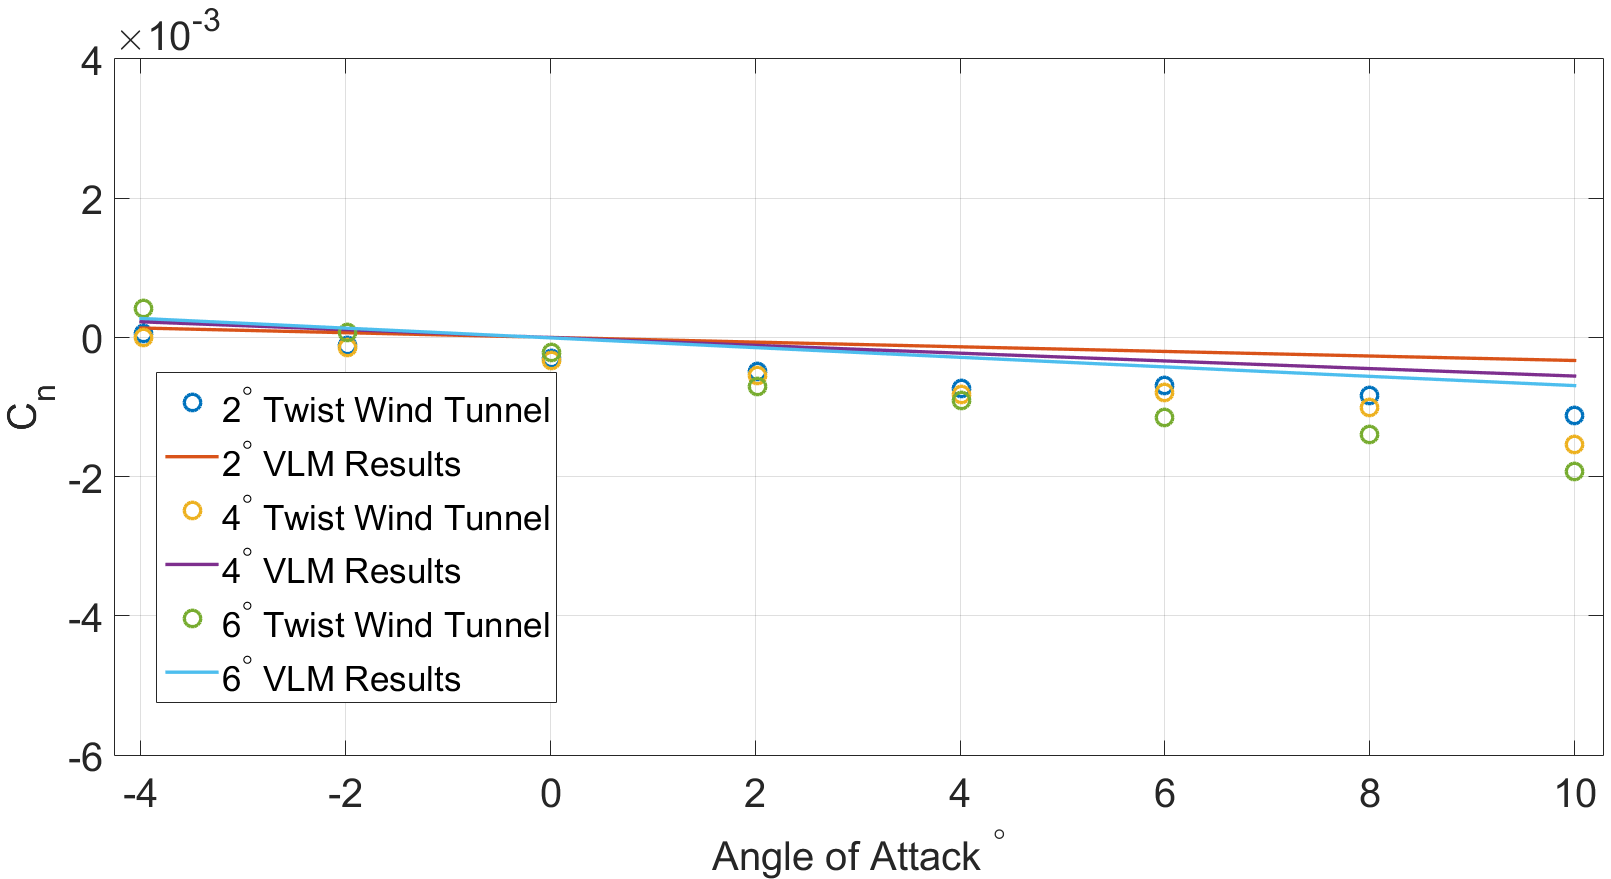
\includegraphics[width=7cm]{Figures/Q2Yaw.png}}
\hfill
\caption{Yaw characteristics at varying A) aileron angle (for rigid model) and B) wing tip twist angle (for flexible model and simulation model), as a function of angle of attack. (dynamic pressure = 2 psf)}
\label{fig:Q2Yaw}
\end{figure}

Figure \ref{fig:Q2Yaw} shows the yawing moment coefficients for the rigid model and the flexible model at a dynamic pressure of 2 psf with surfaces deflected in a similar manner as for the prior asymmetric cases. Note that while the peaks of the yawing moment coefficients are larger in magnitude for the rigid model than the flexible model over the same range of angle of attack, the yawing moment coefficient for the $10^o$ flaperon deflection is minimal in the angle of attack range of 0 to $12^o$ for the rigid model. Above this range and for the larger flaperon deflections, the results in Figure \ref{fig:Q2Yaw} are a mix of proverse and adverse moments which would complicate achieving lateral-directional control harmony with the rigid model. Note that there is a large difference in the magnitude and shape of the curves for the two models. The rigid model is much more jagged; on the other hand, $C_n$ of the flexible model is clearly nearly linear across the angle of attack range tested. The flexible wing exhibits adverse yawing moments arising from drag induced by the asymmetric lift levels of the left and right wings, but the levels are mild and smoothly vary as the angle of attack increases.
The simulation model was able to correctly predict the direction and trend for both the rolling moments and yawing moments, but it did not match the yawing moment as well as it did with the rolling moment. This is to be expected because without a tail or rudder the differential of the wing drag will be the largest contributing factor to yaw. Due to the fact that VLM only calculates the lift-induced drag and excludes other sources of drag, such as the profile drag, which change with varying angle of attack, we would expect that the slope of the simulated yawing moment coefficient curve would be lower than that for the wind-tunnel yawing moment coefficient. There is also a small negative offset in the experimental results relative to the simulation results. VLM only accounts for the lift-induced drag, hence the simulation results always pass through (0,0) where the induced drag is zero. It was assumed that the offset is due to asymmetries in the installation of the flexible model or even the model itself, resulting in left-to-right differences in parasitic drag. If this were the case then 

\begin{figure}[thpb]
\hfill
\subfigure[Rigid model]{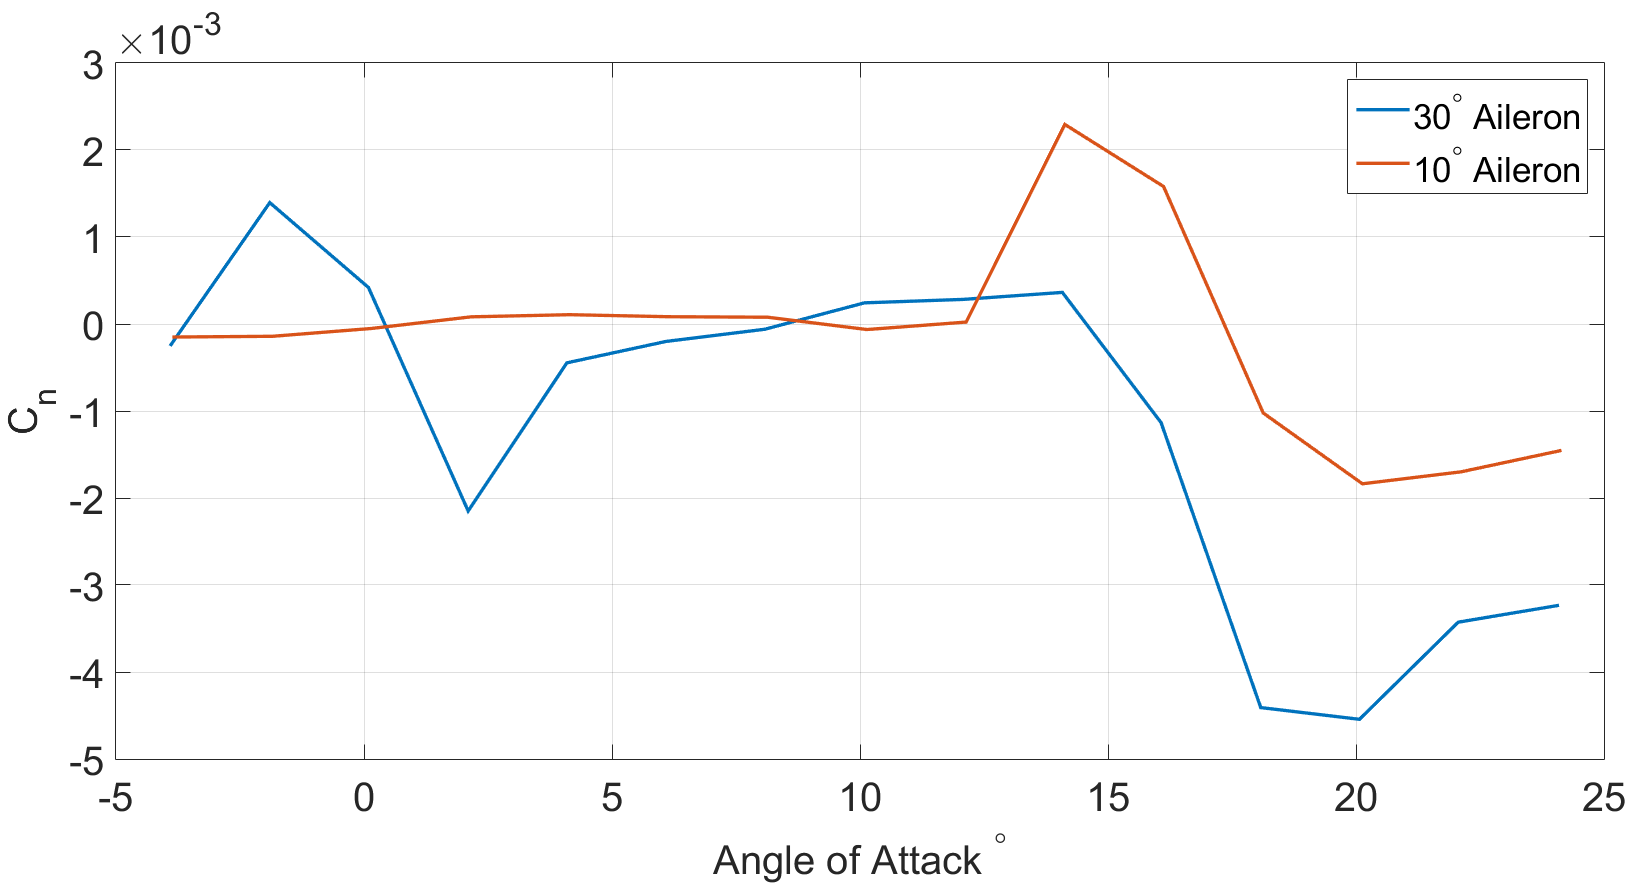
\includegraphics[width=7cm]{Figures/Q3RigidYaw.png}}
\hfill
\subfigure[Flexible model]{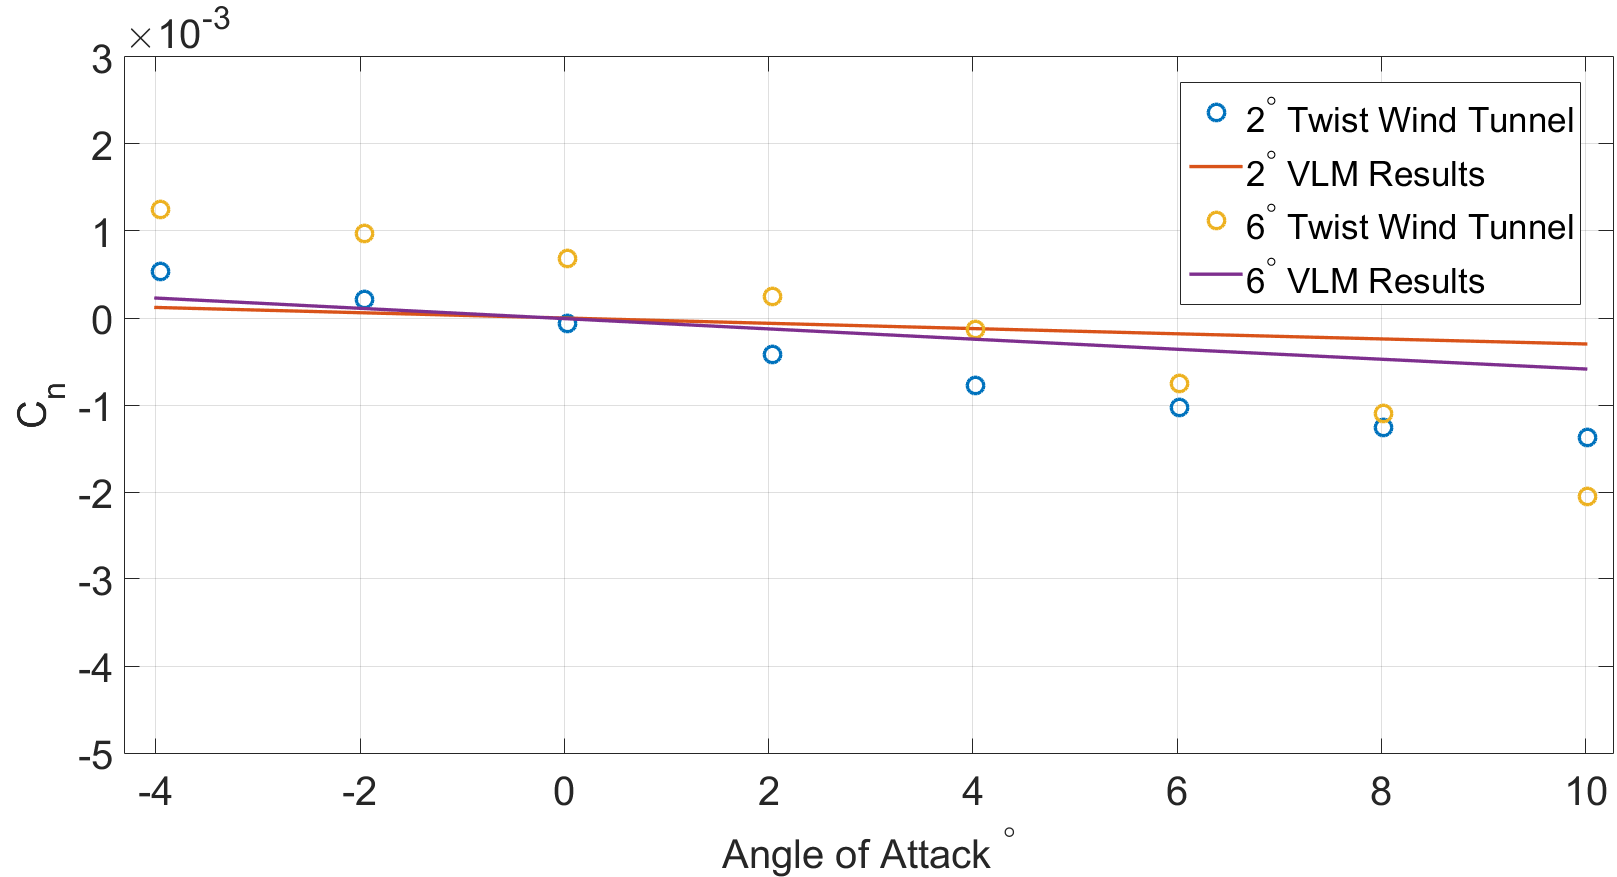
\includegraphics[width=7cm]{Figures/Q3Yaw.png}}
\hfill
\caption{Yaw characteristics at varying A) aileron angle (for rigid model) and B) wing tip twist angle (for flexible model and simulation model), as a function of angle of attack. (dynamic pressure = 3 psf)}
\label{fig:Q3Yaw}
\end{figure}

the zero-crossing point would shift with changes in the air speed, which occurs when the dynamic pressure changes. Figures \ref{fig:Q3Yaw} and \ref{fig:Q4Yaw} show the zero-crossing points shifting with the dynamic pressure, indicating that it is likely the result of a parasitic drag difference.

\begin{figure}[thpb]
\hfill
\subfigure[Rigid model]{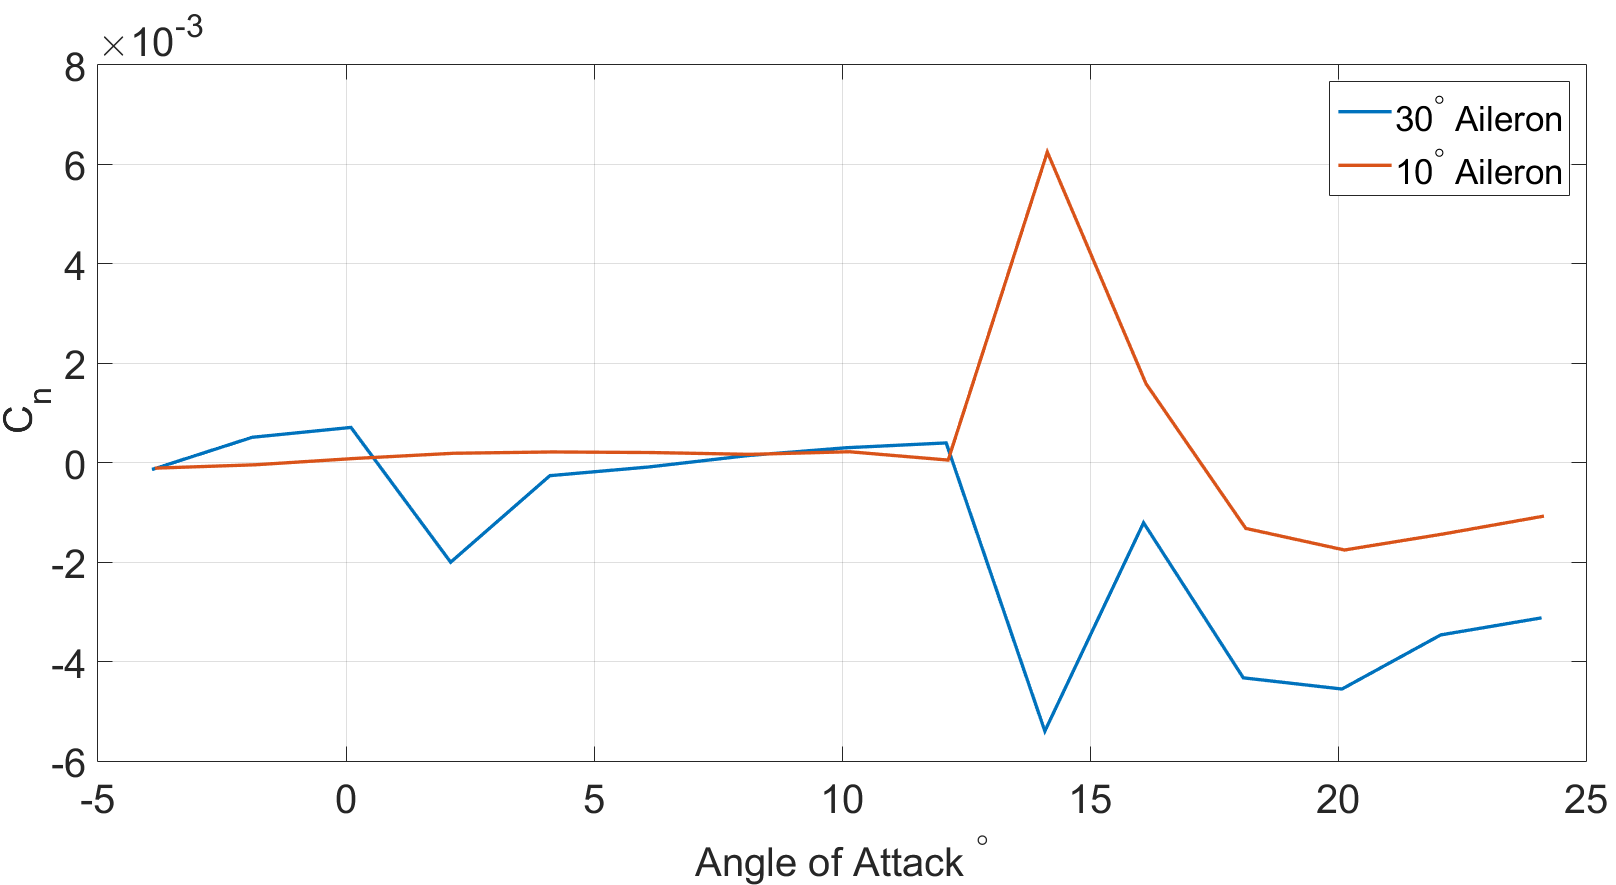
\includegraphics[width=7cm]{Figures/Q4RigidYaw.png}}
\hfill
\subfigure[Flexible model]{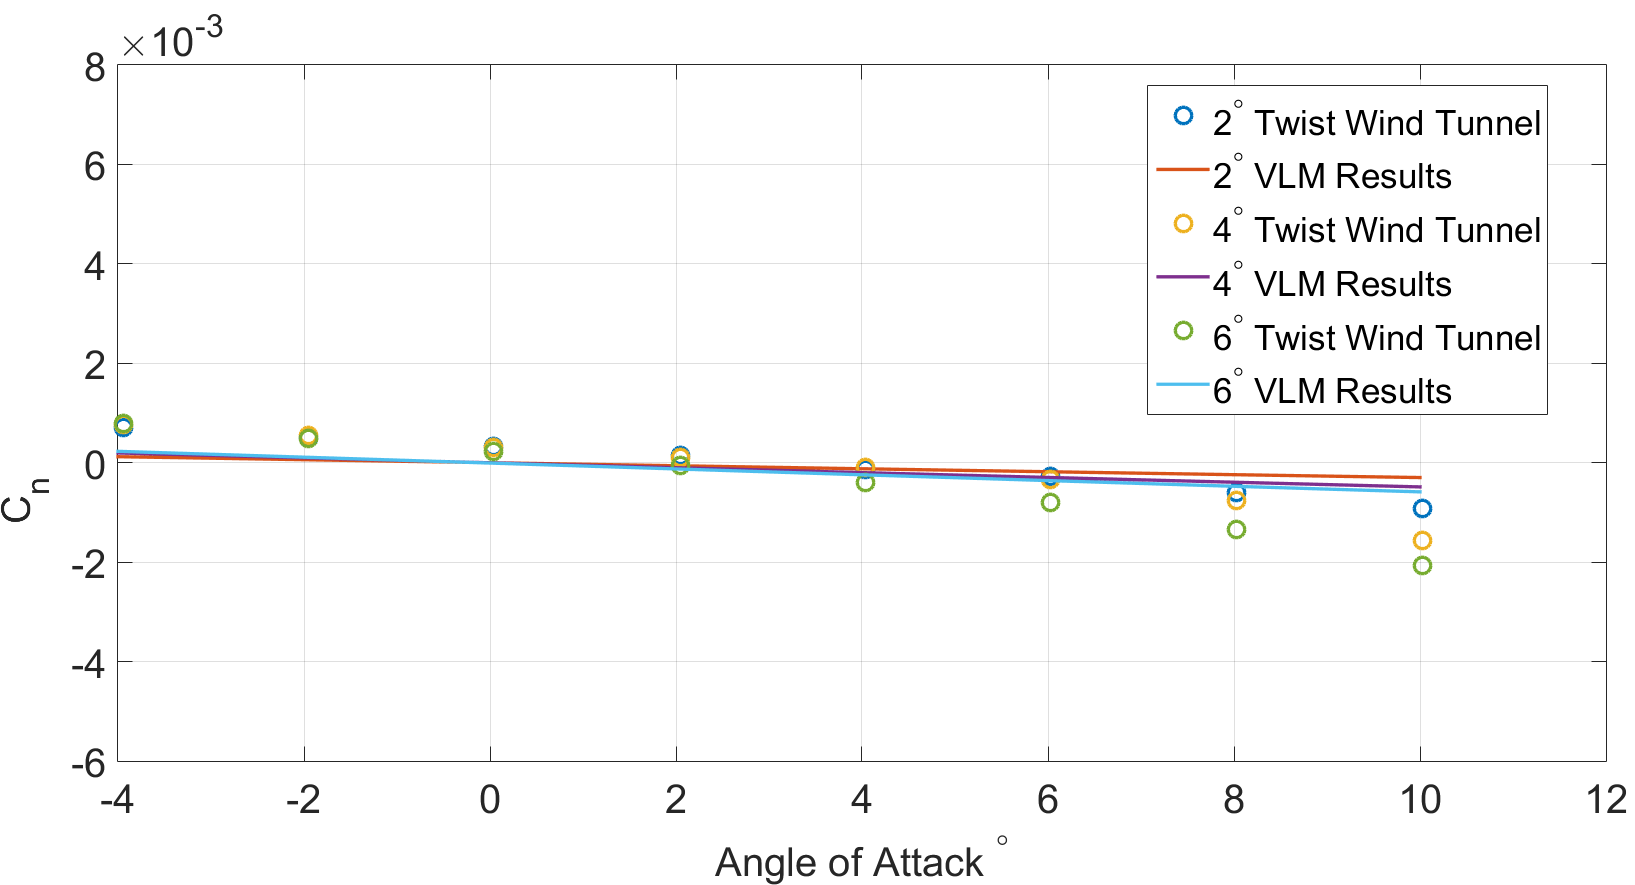
\includegraphics[width=7cm]{Figures/Q4Yaw.png}}
\hfill
\caption{Yaw characteristics at varying A) aileron angle (for rigid model) and B) wing tip twist angle (for flexible model and simulation model), as a function of angle of attack. (dynamic pressure = 4 psf)}
\label{fig:Q4Yaw}
\end{figure}

\subsubsection{Parasitic Drag Inspection}

One theoretical advantage of an active twist system is the potential drag reduction, but we saw in these experiments that the traditional model had lower magnitudes of drag. This was even the case for the flat configurations where there was no twist or flaps which suggest that the difference between the two is the parasitic drag. We estimated the parasitic drag as the drag at the point where there is no lift.

We can see from Figure \ref{fig:parasitic} that the rigid model had a much lower parasitic drag coefficient than either of the flexible models, but the Flex 2 model has a lower parasitic drag than the Flex 1 model. The two flex models are identical in the form of their construction and geometry the primary difference was that the Flex 2 model had all of the reversible joints and attachment points glued. This did not seem to have and visual difference, but it appears it had a quantifiable difference in force response. During testing, it was clear that the Kapton strips used for the skin on the flexible models would flutter and likely resulted in ventilation. It seems likely that the skin selection is a large contributing factor in the increase of the parasitic drag.

\begin{figure}[thpb]
\centering
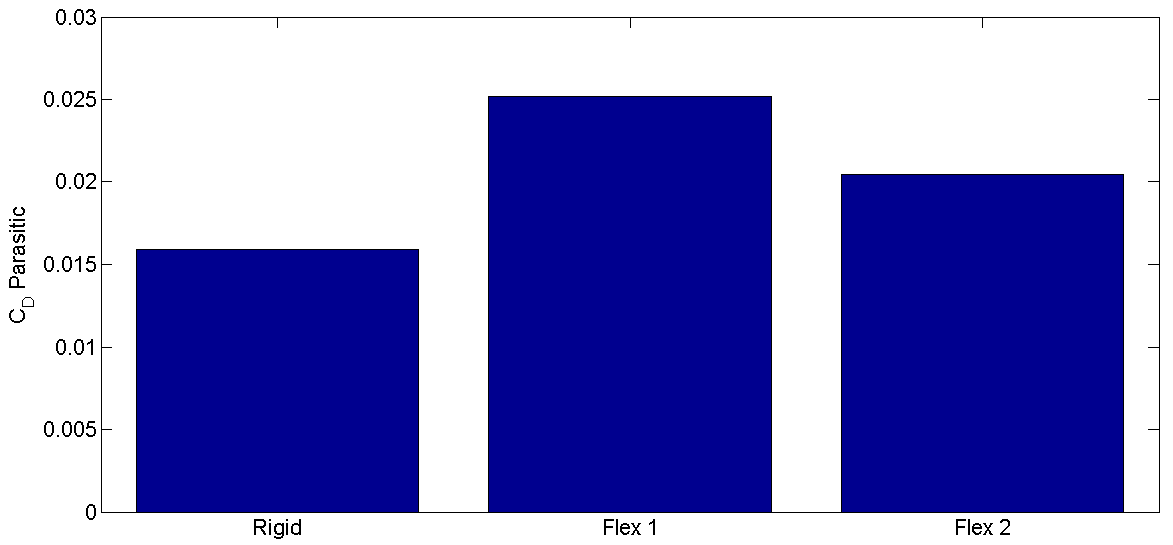
\includegraphics[width=.75\linewidth]{Figures/CdPBulkCompare.png}
\caption{Average of parasitic drag for flat configuration of three models}
\label{fig:parasitic}
\end{figure}

It is likely that the skin friction has a dominate effect in the difference between the flat parasitic drag; however when the flap is actuated or the tip is twisted there is a change in the form friction. We can estimate this by assuming that the skin friction is nearly the same for each configuration and looking at the difference in the parasitic drag. 

\begin{figure}[thpb]
\centering
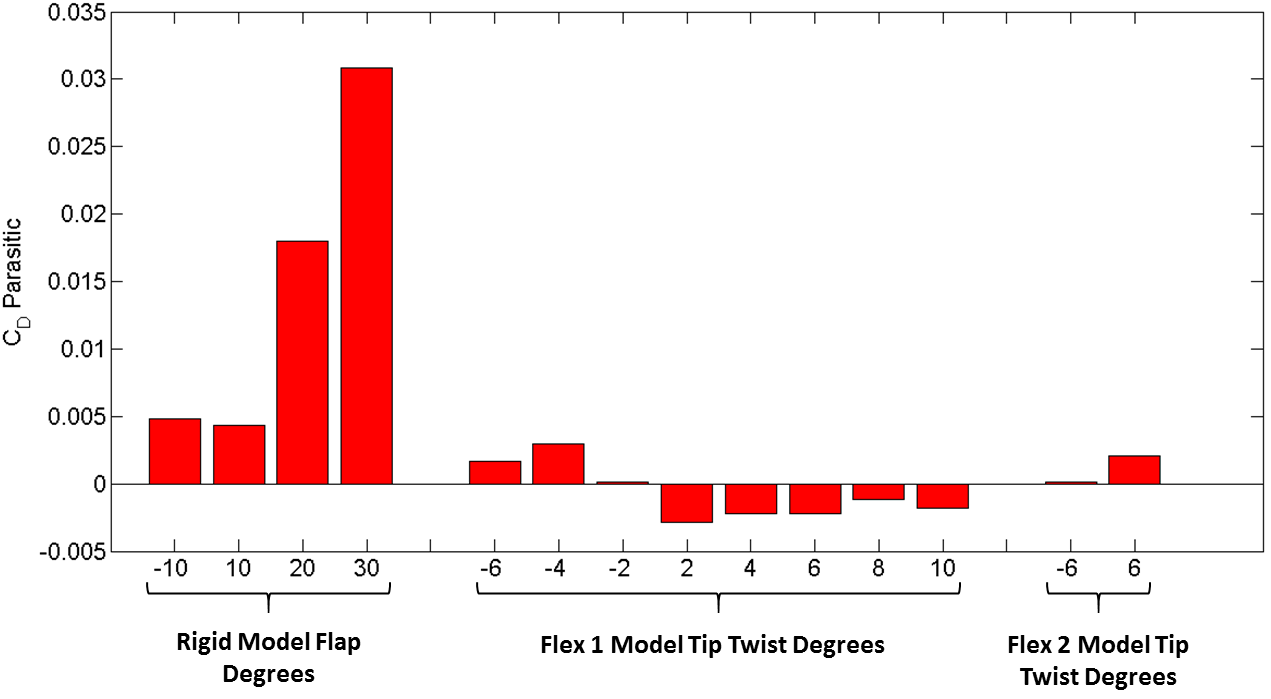
\includegraphics[width=.75\linewidth]{Figures/CdPDiffCompare.png}
\caption{Comparisons of the difference between the flat parasitic drag and the twisted tips or angled flaps}
\label{fig:parasiticDiff}
\end{figure}


Figure \ref{fig:parasiticDiff} shows the difference in the parasitic drag for the flaps and active twist. Overall the difference in parasitic drag is small for the active twist configurations, indeed, when we compare the two most similar configurations, the 6° Tip Twist and 10° Flap that the magnitude of change for the flex models are nearly half that for the flaps.

\subsection{Dynamic Wind Tunnel Results}
\label{sec:DWTR}

One of the more under explored aspects of active twist is the aerodynamic capabilities of active twist. In the earlier section of the symmetric static twist one of the reasons that the $6^o$ tip twist drag increases at a faster rate with respect to $\alpha$ than the comparable $10^o$ rigid flap is that as a control surface active twist has a much larger wetted surface area than the flap which means that it it has a larger form drag but will hit stall latter. While from a static perspective the increased wetted surface area can be an negative at increasing angles of attack there is potential to use the increased surface area as a means to enhance aerodynamic control parameters. In this section we will investigate the capabilities of symmetric active twist as a means of aeroelastic control and validate the modeling technique presented in Section \ref{sec:modeling}.

\begin{figure}[thpb]
\centering
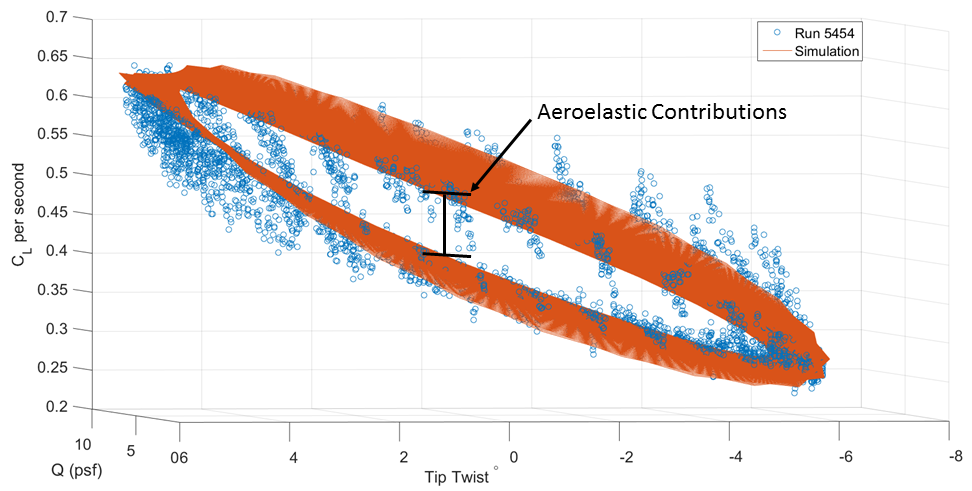
\includegraphics[width=.75\linewidth]{Figures/Run5454CLAeroelastic.png}
\caption{The shape of the simulation matches well with the over all shape of the wind tunnel results. The gap between the top and the bottom is the aeroelastic contributions of the dynamic twist showing the ability to control $C_L$ with the twist rate as well as the tip twist.}
\label{fig:CLRun5454}
\end{figure}

The wind tunnel testing had the tip twist oscillating in a sine pattern at a given frequency between $6^o$ and $-6^o$ tip twist and had the dynamic pressure linearly increasing from $1 psf$ to $7 psf$. To demonstrate the capabilities of the symmetric twist sine wave we will analyze a case study oscillating at $4 Hz$. The simulations were performed using the same parameter shown in Table \ref{tab:vlmConfig}. Figure \ref{fig:CLRun5454} shows that the shape of the aeroelastic simulation matches the wind tunnel results well. The gap shown between top section of the wave form and the bottom section of the wave form is the aeroelastic contributions. While the $C_L$ wave form matches well Figure \ref{fig:CDRun5454}  shows that the drag coefficient does not match very well. The wind tunnel results are much more dispersed and the aeroelastic simulation seems to be representing the floor of the wind tunnel data instead of matching its shape. Of particular interest is the lift to drag ratio because it acts as an effective evaluation of aerodynamic efficiency. Figure \ref{fig:LDRun5454} shows the lift drag ration for the wind tunnel testing and the aeroelastic simulation. The overall shape of the simulation is a decent representation of the shape of the wind tunnel data but it suffers from the same loss in magnitude that the drag coefficient exhibits.

\begin{figure}[thpb]
\centering
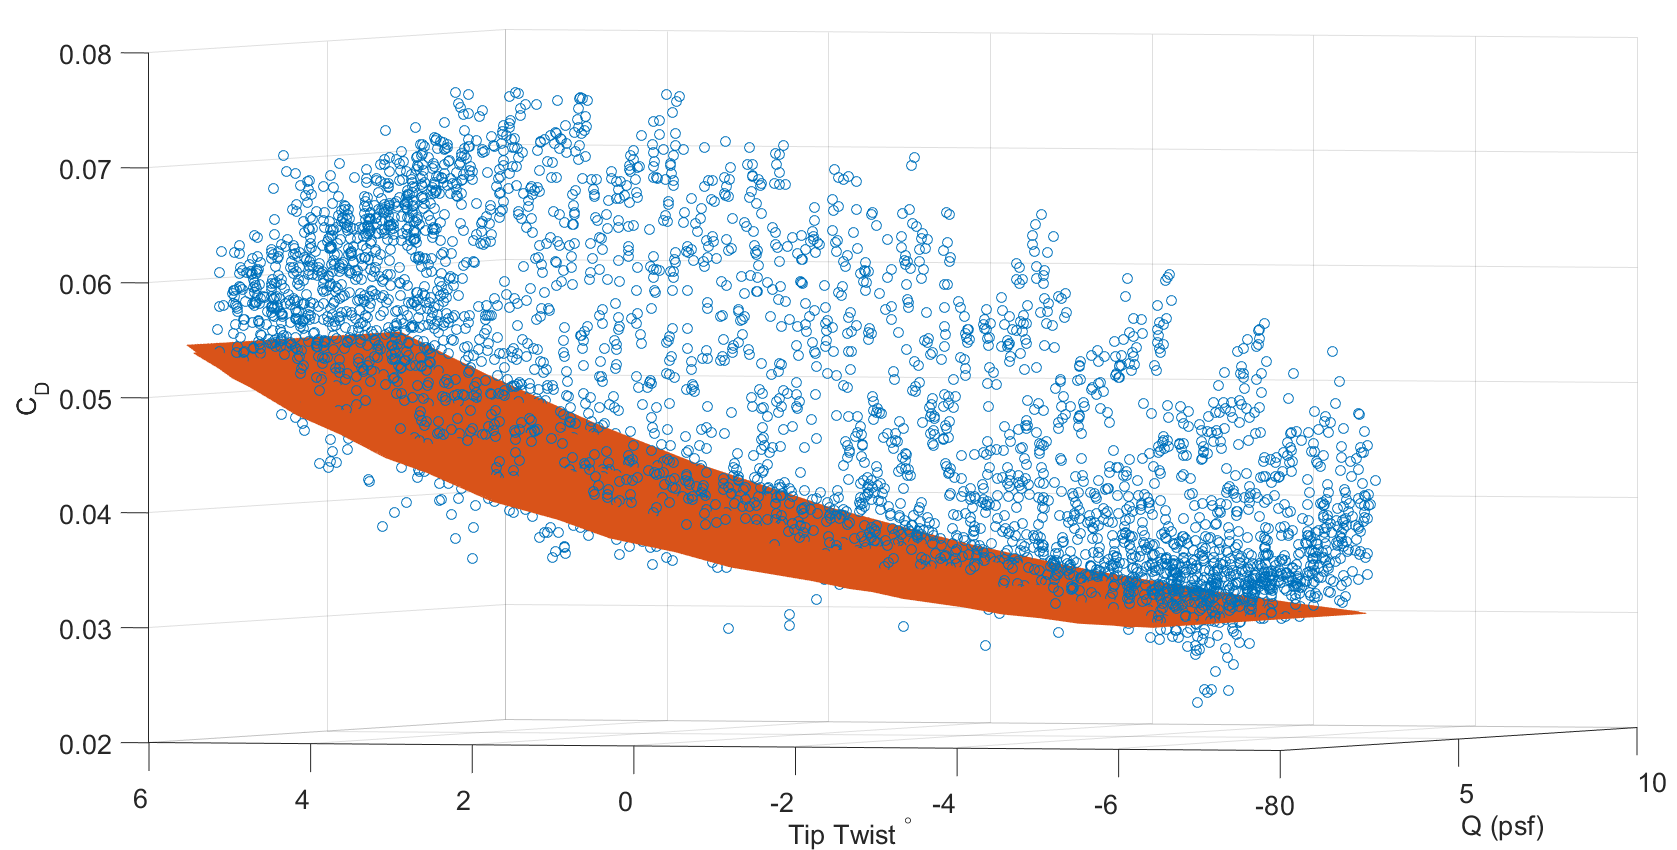
\includegraphics[width=.75\linewidth]{Figures/CD5454.png}
\caption{The simulations results do not match the drag coefficient as well and instead seem to act more as a floor.}
\label{fig:CDRun5454}
\end{figure}

\begin{figure}[thpb]
\centering
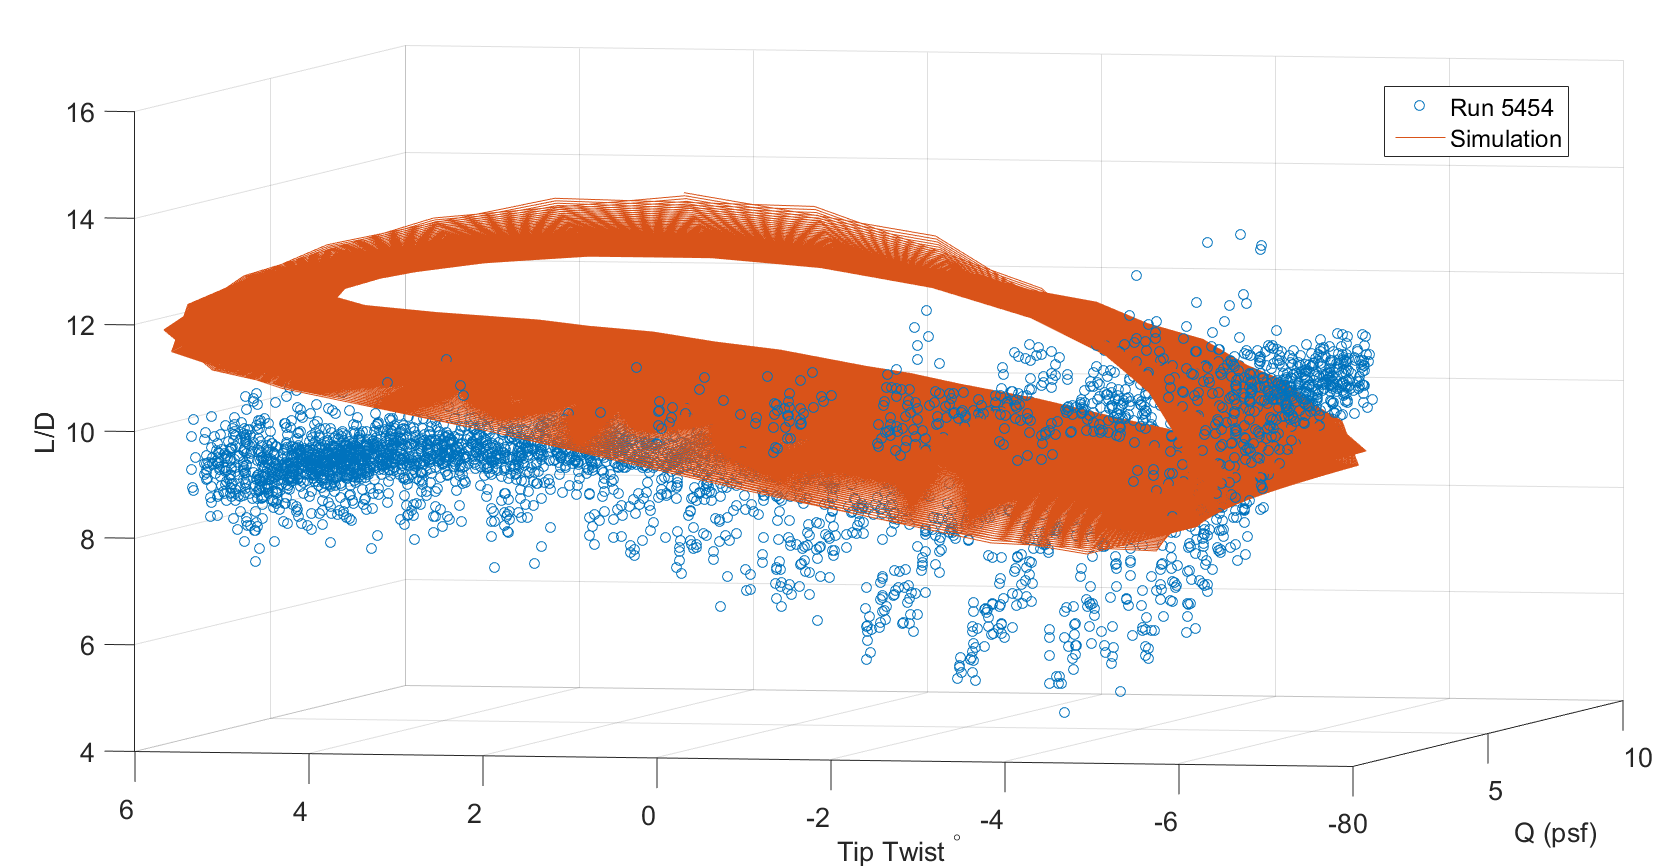
\includegraphics[width=.75\linewidth]{Figures/LD5454.png}
\caption{The simulations results do not match the drag coefficient as well and instead seem to act more as a floor.}
\label{fig:LDRun5454}
\end{figure}

It is possible that the errors displayed in Figures \ref{fig:CLRun5454} to \ref{fig:LDRun5454} are the result of static errors from the bulky fuselage and the small aspect ratio (3) of the aircraft. To investigate the effect of the dynamic active twist the time derivative for the aforementioned parameters. Figure \ref{fig:dCLdtRun5454} shows that the aeroelastic contributions are proportionally much larger for $\frac{dC_L}{dt}$ than they were for $C_L$ in Figure \ref{fig:CLRun5454} and the simulation replicates the wind tunnel data.

\begin{figure}[thpb]
\centering
\includegraphics[width=.75\linewidth]{Figures/diffCL5454.png}
\caption{The shape of the simulation continues to matches well with the over all shape of the wind tunnel results. The aeroelastic contributions are much more dominant for the lift coefficient rate.}
\label{fig:dCLdtRun5454}
\end{figure}

While the largest qualitative difference between Figures \ref{fig:CLRun5454} and \ref{fig:dCLdtRun5454} is that shape is rounder and the aeroelastic contributions are more pounced the time derivative of the drag coefficient shows a dramatic increase in the accuracy of the simulation. Figure \ref{fig:dCDdtRun5454} shows that the simulation matched much better to the shape of the wind tunnel results, with the small exception of the lower right corner around negative six degrees. This suggests that much of the error shown in Figure \ref{fig:CDRun5454} is actually the result of static errors and that the rate of change of the drag coefficient is dominated by the induced drag.

\begin{figure}[thpb]
\centering
\includegraphics[width=.75\linewidth]{Figures/diffCD5454.png}
\caption{The shape of the simulation matches well with the over all shape of the wind tunnel results, suggesting that the rate of change of the drag coefficient is largely due to induced drag}
\label{fig:dCDdtRun5454}
\end{figure}

The rate of change of the lift drag ratio shows good matching with the wind tunnel results as well. This is important because if we were to ignore the desired lift traveling along the path that allowed the rate of change of the lift drag ratio to always be positive would result in an increase in the lift drag rations in time, the range of particular interest for this frequency and for arbitrary lift would be the region between $6^o$ and $4^o$ tip twist. While it is not realistic to ignore the lift requirements of the aircraft this concept is an important one that will be explored more later in this thesis.

\begin{figure}[thpb]
\centering
\includegraphics[width=.75\linewidth]{Figures/diffLD5454.png}
\caption{As a result of the drag rate being able to be matched by the simulation the lift drag ratio rate is matched well by the simulation as well.}
\label{fig:dLDdtRun5454}
\end{figure}

Now that we have a qualitative concept of the affect of the dynamic twist we need to develop a quantitative means of comparing the simulations to the wind tunnel data. To do this we will use the maximum and minimum envelope values as shown in Figure \ref{fig:CLEnvelope} for the lift coefficients and Figure \ref{fig:CDEnvelope} for the drag coefficients. 

\begin{figure}[thpb]
\hfill
\subfigure[Wind Tunnel Envelope]{\includegraphics[width=7cm]{Figures/CLEnvelope-01.png}}
\hfill
\subfigure[Aeroelastic Simulations Envelope]{\includegraphics[width=7cm]{Figures/CLSimEnvelope-01.png}}
\hfill
\caption{$C_L$ envelope for the wind tunnel results and the aeroelastic simulations}
\label{fig:CLEnvelope}
\end{figure}

Figure \ref{fig:PError5454} shows the combined percent error of the maximum and minimum envelopes for the lift and drag coefficients. The percent error was calculated for each envelope (maximum and minimum) separately and then added together to get the cumulative envelope error. The drag coefficient error shown in Figure \ref{fig:PError5454} is actually approaching the maximum expected accuracy for drag given the vortex lattice method. The simulation method takes into account lift induced drag and then an bulk estimate of skin friction which \cite{thomas1985aircraft} states accounts for about $85\%$ of drag. There is also no clear trend line for the drag coefficient but the lift coefficient does show an downward trend in the amount of error in time. This also corresponds to the decreasing of reduced frequency into the quasi-static range. A single test run is not sufficient to make any lasting judgments on the impact of reduced frequency on the overall accuracy. Figure \ref{fig:RFreqvCLEr} shows the reduced frequency against the lift coefficient's percent error against. The colored dots are the time domain percent error, the black line if the least squares best fit while the pink section is the $95\%$ confidence interval, the blue section is the expected operation range for the aircraft. While the maximum error value for the operational area might appear alarming at first it is important to keep in context that $45\%$ of the data points were had less than $15\%$ error in the operational range and a majority of the values that were not came from a single test run. Similar methods such as the one \cite{long2004object} used, which was a full vortex ring method and that they compared to results from \cite{halfman1952experimental} which used a rigid NACA 0012 spanning the whole wind tunnel to approximate an infinite wing that pitched and plunged and a constant rate while the airspeed was kept constant. Long {\it et. al} got errors of four to eight percent for a similar range of testing but with a much more idealized configuration our range is easily twice that but the majority of the values are below the fit line because of the hefty punishment levied by the time domain outliers which would have been less evident in Halfman's configuration because he measured the simple amplitude without the complications of increasing airspeed. At the time of wind tunnel testing it was decided to do the testing by sweeping the airspeed due to time constraints and a desire to explore the aeroelastic coupling at the largest amount of airspeed values.

\begin{figure}[thpb]
\hfill
\subfigure[Wind Tunnel Envelope]{\includegraphics[width=7cm]{Figures/CDEnvelope-01.png}}
\hfill
\subfigure[Aeroelastic Simulations Envelope]{\includegraphics[width=7cm]{Figures/CDSimEnvelope-01.png}}
\hfill
\caption{$C_D$ envelope for the wind tunnel results and the aeroelastic simulations}
\label{fig:CDEnvelope}
\end{figure}

\begin{figure}[thpb]
\hfill
\subfigure[Wind Tunnel Envelope]{\includegraphics[width=7cm]{Figures/CLPercentError-01.png}}
\hfill
\subfigure[Flexible model]{\includegraphics[width=7cm]{Figures/CDPercentError-01.png}}
\hfill
\caption{Lift and drag percent error for the maximum and minimum envelopes of the test run oscillating at $4 Hz$ and an angle of attack of $6^o$}
\label{fig:PError5454}
\end{figure}

\begin{figure}[thpb]
\centering
\includegraphics[width=.75\linewidth]{Figures/ReducedFreqvCLPError-01.png}
\caption{The accuracy of the simulation scales with the reduced frequency}
\label{fig:RFreqvCLEr}
\end{figure}

The ultimate goal of this simulation tool is to be able to be used as a design tool to understand trends and capabilities in a computationally efficient manner and to be able to estimate the control derivatives. To validate this linear step-wise regression was performed using NASA's System IDentification Programs for AirCraft (SIDPAC) \cite{klein2006aircraft} on both the wind tunnel data and the simulated data. The results are shown in Table \ref{tab:WTSystemID} for the most parts the estimated parameters for the simulations matched well with the wind tunnel estimates. For the control derivatives associated with lift and drag coefficients the only ones that showed large errors were very small values that are nearly zero and the $95\%$ confidence interval ranges for the values over lap meaning that there is still a possibility that the simulations value could be a representative of the wind tunnel value. The rate control derivatives have some larger errors on the non primary control derivatives (tip twist as opposed to twist rate) which seems likely to be a result of errors from the simplistic finite derivatives  taken to achieve those values.% The parameters were attempted to fit into Theodorsen's function shown below, where $\rho$ is the density of the wing, $b$ is the span, $x_f$ is the center of twist, $c$ is the cord, $U$ is airspeed, $\alpha$ is the local angle of attack, and $C$ is the reduced frequency based function stratifying the Kutta condition. The acceleration components were of such poor quality they were detrimental to include the values in the table do still fit into the Theodorsen's function and simply suggest that the tip twist and linear extrapolation from there dominates the $\dot{\alpha}$ parameter.

%\begin{equation}
%l = \rho \pi b^2(-(x_f-\frac{c}{2})\ddot{\alpha}+U\dot{\alpha})+\pi \rho U cC(U\alpha+(\frac{3c}{4}-x_f)\dot{\alpha})
%\end{equation}

\begin{table}[h]
\begin{center}
\caption{Wind Tunnel and Simulation System ID}
\label{tab:WTSystemID}
\begin{tabular}{ c|c|c|c|c}
Parameter&Wind Tunnel Estimate&Simulation Estimate&Percent Error& Range Overlap\\\hline
$C_{L_{\theta}}$&0.0257&0.03&$16.6\%$&True\\
$C_{L_{\dot{\theta}}}$&$-3.16e^{-5}$&$-4.97e^{-4}$&$147\%$&True\\
$C_{D_{\theta}}$&$2.39e^{-3}$&0.0016&$32.9\%$&True\\
$C_{D_{\dot{\theta}}}$&$3.38e^{-6}$&$-9.79e^{-7}$&$129\%$&True\\
$\frac{dC_{L_{\theta}}}{dt}$&$5.65e^{-5}$&0.0174&$208\%$&False\\
$\frac{dC_{L_{\dot{\theta}}}}{dt}$&$0.027$&$0.0308$&$14.1\%$&True\\
$\frac{dC_{D_{\theta}}}{dt}$&$-7.68e^{-5}$&$-3.82e^{-3}$&$4.87e^3\%$&False\\
$\frac{dC_{D_{\dot{\theta}}}}{dt}$&$2.1e^{-3}$&$1.59e^{-3}$&$24.3\%$&False\\
\end{tabular}
\end{center}
\end{table}  

\subsubsection{Stall Mitigation}

\begin{figure}[thpb]
\centering
\includegraphics[width=0.75\linewidth]{Figures/StallMitigationCompare.png}
\caption{Comparisons of the test for stall mitigation at various angles of attack and their expected values from Figure \ref{fig:CL}}
\label{fig:SM}
\end{figure}

The lift data of Figure \ref{fig:CL} presents an interesting possibility to use active twist for stall mitigation at a given angle of attack. For example, at a tip twist of 10o and an angle of attack of $10^o$, the flexible model has begun to stall; however, while maintaining the angle of attack, the twist could be reduced (e.g., to 4 o or below) to avoid stall. A brief experiment was run to show that stall mitigation was actually possible, and the results compared favorably to the trends shown in Figure \ref{fig:CL}.
To test the active twist capability of stall mitigation, we started at given angle of attack and a tip twist of $10^o$. Twist was then reduced by $2^o$ and maintained at the new value for ten seconds. Figure 16 shows the results of the stall mitigation tests compared to the expected values. We can see that for all the angles of attack other than $14^o$, we were able to mitigate the stall effects by varying the twist. In fact, in these cases we were able to observe stall-induced trailing edge flutter of the wing skin, and the trailing edge flutter for the $10^o$ angle of attack visually stopped at $6^o$ of twist, confirming what the data indicate in Figure \ref{fig:SM}. It is also interesting to note that the lift coefficients from the stall mitigation tests were consistently 0.5 higher than the expected values. Of course, more runs would be needed to show that changing twist to alleviate stall would actually result in a higher lift coefficient, but it is interesting nonetheless.


%%%%%%%%%%%%%%%%%%%%%%%%%%%%%%%%%%%%%%%%%%%%%%%%%%%%%%%%%%%%%%%%%%%%%%%%%%%
\chapter{Control}
%\section{Structural Stability Control of Lattice Structure}
The control of morphing aircraft has been a critical limiting factor in the adoption of this technology into industrial applications. Much like the simulation methodology it is necessary to develop the structural control aspects of the aeroelastic control before moving to the fully coupled system. To address these issues I start by trying to develop controllers that take advantage of the underlying configuration of the structure.

\section{Structural Decentralized Control}
\label{sec:decentral}
One of the primary issues when developing structural control is the shear demensionality that is associated with a large (and even not that large) lattice based structures. One of the primary advantages of using the lattice-based approach is that each voxel can be individually characterized and considered a physical ``finite element'' \cite{calisch2014physical}. Therefore, the behavior of the entire wing structure could be predicted by assembling the required series of elementary voxels. 

As a practical example of the proposed approach, we will consider a single long array of octahedron voxels anchored to a rigid base representing a minimalistic wing attached to the planes fuselodge. Figure \ref{fig:interconnected} shows an example of a single interconnected array of voxel substructures. The proposed model consists of two types of voxels: {\it active voxels} (with control authority), which could perform as an active functional component with actuation capability,  and {\it passive voxels} (without control authority). The goal is that active voxels could suppress vibration due to external disturbances, and therefore, improve the overall performance of the structure. It should be noted that for easy manipulation, the active and passive voxels have identical connectors and require identical assembly techniques.  

\begin{figure}[thpb]
\centering
\includegraphics[width=0.75\linewidth]{Figures/exampleInterconnectedStructure.png}
\caption{A single long array of cuboctahedron voxels. Red indicates an active voxels and green a passive one.}
\label{fig:interconnected}
\end{figure}

The voxels that we are proposing to use as the basis for the space structure have already been created and tested.\cite{jenett2016meso} We will use the primary bending modes of the voxels as a means of creating a low order model. This low order model then allows us to create a large scale model of the proposed space structure. For very large scale structures even with a low order model, like the one we are proposing, the problem can quickly become intractable. Deminsionality issues are a primary motivation for the creation of decentralized control\cite{bakule2008decentralized}, this and the inherent structure of the lattice make it an excellent choice for decentralized control.

\subsection{Low Order Modeling of a Cuboct Voxel}
\label{sec:model}
To obtain a low-order spring-mass-damper model of a voxel substructure, we performed a lab-based dynamics and vibration test. The voxel was rigidly attached to a vibration isolating optical table and loaded at the top. The modal response of the voxel during unloading was monitored using a Laser Vibrometer, which was mounted on the same vibration isolation optical table to minimize outside interference. The laser was focused on the mounting nodes for measurement. Figure \ref{fig:setUp} shows the experimental setup on the left and the voxel on the right. Figure \ref{fig:setUpD} schematically shows the loading/unloading approach.

\begin{figure}[thpb]
\centering
\includegraphics[width=0.75\linewidth]{Figures/experimentalSetup.png}
\caption{Experimental setup (left) and a single voxol clamped on teh optical table (right)}
\label{fig:setUp}
\end{figure}

\begin{figure}[thpb]
\centering
\includegraphics[width=0.25\linewidth]{Figures/experimentalSetupDiagram.png}
\caption{Schematic representation of the experimental procedure. }
\label{fig:setUpD}
\end{figure}
Figure \ref{fig:FFTandQ} shows the frequency domain of the voxel, measured at the five nodes connecting the carbon fiber struts. The first harmonic mode (see insert in Figure \ref{fig:FFTandQ}) corresponds to the first bending mode of the voxel. Equation \ref{eqn:Q} predicts the quality factor using the maximum frequency and the full width at half maximum.

\begin{equation}
Q = \frac{f_{max}}{\Delta f}
\label{eqn:Q}
\end{equation}
The quality factor can be related to the damping of the system through,
\begin{equation}
c = 4 \sqrt{k M} Q \,.
\label{eqn:Q2c}
\end{equation}

\begin{figure}[thpb]
\centering
\includegraphics[width=0.75\linewidth]{Figures/FFTandQ.png}
\caption{Frequency domain of the cuboctahedron voxel, measured at the five nodes connecting the carbon fiber struts. The lowest harmonic order is used to find the quality factor.}
\label{fig:FFTandQ}
\end{figure}
The mass of the voxel $M=1.01$ kg, is used to predict the appropriate spring constant $k$ associated with the primary bending mode and it is given by
\begin{equation}
k = f_{max}^2 M = 771.7 \, {\mbox N/m}
\label{eqn:kfm}
\end{equation}
which results in a damping of $c = 97.41 \frac{N}{ms}$. It is also of interest that as the frequency increases the peaks continue to spread out and diverge into multiple individual peaks, which is evidence of the variations between beams and that the interface between the beams plays a substantial role in the behavior of the structure at the higher modes.

The equations of motion for the assembled space structure is obtained using the low order spring-mass-damper voxel models, as follows,
\begin{equation}
\begin{array}{l}
\mathcal{M} \ddot{\eta}(t) + \mathcal{C} \dot{\eta}(t) + \mathcal{K} \eta(t) = \mathcal{B} u(t) + \mathcal{D} w(t)
\end{array}
\label{eqn:smdSys}
\end{equation}
where $\eta (t)$, $\dot{\eta} (t)$, and $\ddot{\eta} (t)$ denote respectively the displacement, velocity and accelration of the voxels, $u (t)$ represents the active voxels whose locations are indicated in $\mathcal{B}$, $w (t)$ denotes the disturbance inputs, with intensity $W >0$, applied to the voxel structure. We assume there is a total of $n$ voxels, among them $m$ active voxels. The structural matrices $(\mathcal{M}, \mathcal{C}, \mathcal{K})$ have dimensions $n \times n$ and can be defined as
\begin{equation}
\begin{bmatrix}m&0&0&0&\dots&0\\0&m&0&0&\dots&0\\0&0&m&0&\dots&0\\\vdots&\vdots&\vdots&\vdots&\ddots&\vdots \\0&0&0&0&\dots&m\end{bmatrix} \,,\;
\begin{bmatrix}2c&-c&0&0&\dots&0\\-c&2c&- c&0&\dots&0\\0&-c&2c&-c&\dots&0\\ \vdots&\vdots&\vdots&\vdots&\ddots&\vdots \\0&0&0&0&\dots&c\end{bmatrix} \,,\;
\begin{bmatrix}2k&-k&0&0&\dots&0\\-k&2k&-k&0&\dots&0\\0&-k&2k&-k&\dots&0\\ \vdots&\vdots&\vdots&\vdots&\ddots&\vdots \\0&0&0&0&\dots&k\end{bmatrix} \,.
\label{eqn:EOS}
\end{equation}
Then, Equation (\ref{eqn:smdSys}) can be rewritten in the state-space representation as follows,

\begin{equation}
\dot{x} (t) = A x(t) + B u(t) + D w(t)
\label{sigma1}
\end{equation}
where $x = [\eta^t \;\; \dot{\eta}^t]^t$ denotes the states, and

\begin{equation}
A = \begin{bmatrix}0&I\\-\mathcal{M}^{-1} \mathcal{K}&-\mathcal{M}^{-1} \mathcal{C} \end{bmatrix}\,,\; B = \begin{bmatrix}0\\\mathcal{M}^{-1} \mathcal{B} \end{bmatrix}\,,\;D = \begin{bmatrix}0\\\mathcal{M}^{-1} \mathcal{D} \end{bmatrix} .
\label{eqn:stateM}
\end{equation}
We assume the actuator dynamics can be described by
\begin{equation}	\label{act1}
\dot{u}_i (t) = a_i u_i (t) + b_i v_i (t) \,,\;\; i = 1,2,\dots, m \,,
\end{equation}
where $(a_i , b_i)$ are known, $[v_1 \,\, v_2 \, \cdots \, v_m]^{t} = v$ are the commanded inputs, and $[u_1 \,\, u_2 \, \cdots \, u_m]^{t} = u$. Then, (\ref{act1}) can be expressed in a compact matrix form as
\begin{equation}	\label{act2}
\dot{u} (t) = A_u u(t) + B_u v(t) \,,
\end{equation}
where $A_u$ and $B_u$ are diagonal matrices with entries $a_i$ and $b_i$, respectively. In this study, we consider that each control input $u_i$ is bounded by its practical limitation. Hence, the proposed decentralized control is to design a novel bounded input controller to suppress the excessive structural vibration for (\ref{sigma1}).    

\subsection{Decentralized Model Formulation}
\label{sec:decentral}
To generate the decentralized control formulation we will follow the procedure for Type II overlapping control presented by $Ze\check{c}evi\acute{c}$\cite{zevcevic2005new} and $\check{S}iljak$\cite{siljak2011decentralized}, and extend it to include the actuator dynamics. To start, we first combine (\ref{sigma1}) and (\ref{act2}) to form an augmented system as follows,
\begin{equation}	\label{aug1}
\Sigma : \;\; \dot{\bar{x}} (t) = \bar{A} \bar{x}(t) + \bar{B} v(t) + \bar{D} w(t)
\end{equation}
where the combined state vector $\bar{x}=[x^t \;\; u^t]^t$, and the system matrices are given by
\[
\bar{A} = \left [
\begin{array}{cc}
A & B \\
0 & A_u
\end{array}
\right ]\,,\;\bar{B} = \left [
\begin{array}{c}
0 \\
B_u
\end{array}
\right ] \,,\;\bar{D} = \left [
\begin{array}{c}
D \\
0
\end{array}
\right ] \,.
\]

Next, depending on where the active voxels are being placed, we need to re-order the sequence of combined state vector $\bar{x}$ into, \\e.g., $[\eta_{1}^t \; \dot{\eta}_{1}^t \;u_1 \; \eta_{2}^t \; \dot{\eta}_{2}^t \;u_2 \;\ldots \eta_{m}^t \; \dot{\eta}_{m}^t \;u_m \;\eta_{m+1}^t \; \dot{\eta}_{m+1}^t \ldots]^t$. Subsequently, all thirsty matrices, i.e. matrices in bar, $(\bar{A}, \bar{B}, \bar{D})$ need to be adjusted accordingly. Finally, by following the procedure presented in \cite{zevcevic2005new,siljak2011decentralized}, the matrices $(\bar{A}, \bar{B}, \bar{D})$ can be transformed into an overlapping description $(\hat{A}, \hat{B}, \hat{D})$ as follows,
\begin{equation}
\begin{matrix}
\hat{A} =\left [
\begin{array}{cc|cc|cc|c}
A_{11}&A_{12}&0&0&0&\dots&0\\A_{21}&A_{22}&0&A_{23}&0&\cdots&0\\\hline A_{21}&0& A_{22}&A_{23}& 0&\cdots&0\\0&0&A_{32}&A_{33}&0&A_{34}&\cdots\\\hline0&0&A_{32}&0&A_{33}&A_{34} &\cdots\\\vdots&\vdots&\vdots&\vdots&\vdots&\vdots&\ddots
\end{array}\right ]\,,\; 
\hat{B} = \left [\begin{array}{c|c|c|c}
0&0&\cdots&0\\
b_{1} &0&\cdots&0\\\hline 0&0&\cdots&0\\0&b_{2}&\cdots&0\\\hline 0&0&\cdots&0 \\
\vdots & \vdots & \vdots & \vdots
\end{array}\right ]\\\,,\;
\hat{D} = \left [\begin{array}{c|c|c|c}
D_{1}&0&\cdots&0\\
0&0&\cdots&0\\\hline 0&D_{2}&\cdots&0\\0&0&\cdots&0\\\hline 0&0&\cdots&0 \\
\vdots & \vdots & \vdots & \vdots
\end{array}\right ] .
\end{matrix}
\label{eqn:hatM}
\end{equation}
It should be noted that these matrices meet the requirements set in $\check{S}iljak$ \cite{siljak2011decentralized} as shown below,
\begin{equation}
V \bar{A} = \hat{A}V \;,\;\; V \bar{B} = \hat{B}\;,\;\;V \bar{D} = \hat{D}\,,
\end{equation}
where
\begin{equation}
V = \begin{bmatrix}
I_{1}&0&0&\cdots&0\\
0&I_2&0&\cdots&0\\
0&I_2&0&\cdots&0\\
0&0&I_3&\cdots&0\\
\vdots&\vdots&\vdots&\ddots&\vdots\\
0&0&0&0&I_n
\end{bmatrix} .
\end{equation}
In compact form, the resulting new state-space equation with overlapping states can be described by
\begin{equation}
\hat{\Sigma} : \;\; \dot{\hat{x}}(t) = \hat{A}\hat{x}(t) + \hat{B}v(t) + \hat{D}w(t) \,.
\label{eqn:hatSys}
\end{equation}
For large structures, the number of states causes the problem to be intractable making it necessary to not only create a problem formulation that will result in a controller that can be implemented in a decentralized manner, but to solve the LMI in a decentralized manner. To achieve this, we will formulate the decentralized control problem by focusing on the diagonal subblocks of $\hat{A}$ in (\ref{eqn:hatM}).  

\subsection{LMI-based Constrained Input-Output Optimization Problem}
\label{sec:LMI}
In this section, I formulate the input and output constrained optimization problem for large space structures in the framework of decentralized control. We should first note that input constraints in (\ref{sigma1}) are in fact converted into state constraints in (\ref{eqn:hatSys}), which can then be shown to be equivalent to output constraints by introducing those states as part of control outputs. Consider the following decentralized models derived from (\ref{eqn:hatSys}),

\begin{equation}
\hat{\Sigma}_i\;:\; \left \{
\begin{array}{l}
\dot{\hat{x}}_i (t) = \hat{A}_i \hat{x}_i (t) + \hat{B}_i v_i (t) + \hat{D}_i w(t) \\
y_i (t) = \hat{H}_i x_i (t) \,,\;\; i = 1,2,\dots, m
\end{array}
\right .
\label{eqn:sys}
\end{equation}
where $\hat{\Sigma}_i$ is the $i$th substructure that is controlled by an active voxel $v_i$ located at $\hat{B}_i$. In addition, $y_i$ denotes the control outputs, which can be used to monitor both the local structural responses and the control input $u_i$. Furthermore, the system matrices are given by
\[
\hat{A}_i = \left [
\begin{array}{cc}
A_{i,i} & A_{i,i+1} \\
A_{i+1,i} & A_{i+1,i+1}
\end{array}
\right ] \,,\;\hat{B}_i = \left [
\begin{array}{c}
0 \\
b_i
\end{array}
\right ] \,,\;\hat{D}_i = \left [
\begin{array}{c}
D_i \\
0
\end{array}
\right ] \,,\;\hat{H}_i = \left [
\begin{array}{cc}
H_i & 0 \\
0& 1
\end{array}
\right ] \,.
\]
Note that $H_i$ indicates interested structural response locations at $\hat{\Sigma}_i$, and "1" in $\hat{H}_i$ corresponds to where $u_i$ is located. One critical aspect of decentralized control for large systems is the diagonal dominance of $\hat{\Sigma}$, which makes the control design much tractable since it only involves designing for a subsystem of smaller dimension, such as $\hat{\Sigma}_i$. 

It should be noted that, in $\hat{\Sigma}_i$, constraints on the control inputs $u_i$ are converted into the constraints on output $y_i$, and the allowable control authority is known apriori. Moreover, since our overall control design objective is to suppress the vibrational motion as much as possible, it is practical to pre-set an acceptable or desirable level of structural vibration as design criteria. Now, we can formulate the output covariance constrained optimization problem, which can then be solved as a standard $\mathcal{H}_2$ performance problem \cite{zhu1997convergent}. Also, the existence of such solution can be determined by checking if a feasible solution exists to a coupled linear matrix inequalities (LMIs) \cite{swei2015lmi}. Therefore, the numerically efficient LMI-based convex optimization tools and algorithms can be applied for control design analysis and synthesis. The following theorem contains the main result.

\noindent
\textbf{Theorem 1:} \textit{Consider the system $\hat{\Sigma}$ described in (\ref{eqn:hatSys}). Suppose $\bar{Y}>0$ and $\bar{U}>0$ are known. The output covariance constrained optimization problem is solvable, if there exist matrices $G_i$ and positive definite symmetric matrices $Z_i$, $i=1,2,\dots,m$, that minimize the output covariance performance cost}
\begin{equation}	\label{eqn:LMImin}
\underset{G,Z}{min}\quad trace\,(\,H_i Z_i H_{i}^{t}\,)\,,\quad i = 1,2,\dots, m\,,
\end{equation}
\textit{subject to}
\begin{equation}
\begin{bmatrix}
\hat{A}_i Z_i+Z_i \hat{A}_{i}^{t}+G_i^t \hat{B}_{i}^t+\hat{B}_i G_i &\hat{D}_i W^{\frac{1}{2}}\\\star&-I
\end{bmatrix}<0\,, \quad i = 1,2,\dots, m \,,
\label{eqn:LMILap}
\end{equation}
\begin{equation}
\begin{matrix}
\bar{Y}- \left [ \begin{array}{cc} H_i & 0 \end{array} \right ] Z_i \left [ \begin{array}{c} H_i \\ 0 \end{array} \right ] \,\geq 0 \,, \quad i = 1,2,\dots, m \,, \\
\bar{U}- \left [ \begin{array}{cc} 0 & 1 \end{array} \right ]Z_i \left [ \begin{array}{c} 0 \\ 1 \end{array} \right ] \,\geq 0 \,, \quad i = 1,2,\dots, m \,.
\end{matrix}
\label{eqn:LMIConst}
\end{equation}
\textit{If a feasible solution exists to the above LMIs, then the full state feedback control law is given by} 
% {There exists a stabilizing controller of the form}
\begin{equation}
v(t) = \hat{K} \hat{x}
\end{equation}
\textit{where $\hat{K}$ is of the form}
\begin{equation}
\hat{K} = \begin{bmatrix}
K_{11}&K_{12}&0\\0&K_{22}&K_{23}\\&&&\ddots
\end{bmatrix}
\label{eqn:Khat}
\end{equation}
\textit{and}
\begin{equation}
\begin{bmatrix}
K_{i,i}&K_{i,i+1}
\end{bmatrix}=G_i Z_i^{-1} \,.
\end{equation}
\noindent
{\bf Proof:} The proof combines results from $Ze\check{c}evi\acute{c}$\cite{zevcevic2005new} for decentralized modeling and control architecture, and {\it Swei et al.} \cite{swei2015lmi} for output covariance constrained optimization.

\subsection{Proposed Structure Configuration and Simulation Setup}
\label{sec:struct}
One of the proposed applications for active twist technology mentioned in Section \ref{sec:struct} are HALE aircrafts. For HALE's it is critically important to have large lifting surfaces to allow for low flight speeds in high altitudes. With that in mind I propose an 200 voxel long array that will simulate an half wingspan. Each voxel strut is 0.2m long, hence resulting in a voxel length of about 0.283m, which results in an wing half span of approximately 57m which is of comparable wingspan as the HALE proposed by \cite{goraj1999design}.

An important part of the formulation of the decentralized structural control model is the selection of the actuation/sensor locations and the partitioning of the full model into smaller section. For simplicity of the models, the actuation points were selected to be evenly distributed through the whole structure, for example, if there were 20 active voxels then there would be ten voxels between each active voxel. The boundaries between each active voxel are chosen to be exactly half way between as is shown in Figure \ref{fig:simSetup}.

\begin{figure}[thpb]
\centering
\includegraphics[width=1\linewidth]{Figures/SimulationSetup.png}
\caption{Example of the equally spaced active voxels and the split up of the decentralized control sections}
\label{fig:simSetup}
\end{figure}

The simulation is set up to have the long beam space structure be rigidly attached to the base forming a cantilevered beam where a disturbance is placed at the tip and is in the form of a chirp of length $100\mu s$ and magnitude of one newton of force. While this simulation is not representative of the aeroloading that we might expect it does provide an convenient mechanism to test the decentralized control and resulting control authority from various actuation points that will be important to build up to the whole aeroelastic control. 

\begin{figure}[thpb]
\centering
\includegraphics[width=0.75\linewidth]{Figures/UnControlledPosition-01.png}
\caption{The uncontrolled position provides a reference for how much the voxels oscillate and how fast the disturbance propagates through the system}
\label{fig:UCPos}
\vspace*{\floatsep}
\includegraphics[width=0.75\linewidth]{Figures/Position40Controlled12_10_2016.png}
\caption{The controlled position peak from the disturbance is nearly one third that of the uncontrolled system}
\label{fig:CPos}
\end{figure}

\subsection{Simulation Results}
\label{sec:results}
To study the effectiveness of the proposed we designed and simulated the decentralized controllers on the structure proposed in Section \ref{sec:struct} with 25, 40, and 50 active voxels. We used the approach proposed by SeDuMi and YALMIP \cite{lofberg2004yalmip} to solve the LMIs presented in Section \ref{sec:LMI}. The same weighting matrices were used for all of the simulations to try and make them as comparable as possible. This can be done without fear of stability issues because the off-diagonal components for each model are identical therefore the selected Q that meets the stability requirement for a single case applies to all of them. The simulations were run for 20 seconds using MATLAB's ODE45 solver with commanded time steps of $1ms$.

\begin{figure}[thpb]
\centering
\includegraphics[width=0.75\linewidth]{Figures/UncontrolledVelocity.png}
\caption{The uncontrolled velocity shows how much the initial disturbance dominates the behavior of the system}
\label{fig:UCVel}
\includegraphics[width=0.75\linewidth]{Figures/Velocity40Controlled12_10_2016.png}
\caption{The controlled velocity shows a similar peak reduction to the position plots and a more dramatic reduction in the remnant velocity oscillations}
\label{fig:CVel}
\end{figure}

We can gain a basic understand of the performance of our system from the behavior of the uncontrolled simulation.From Figure \ref{fig:UCPos} we can see the disturbance propagate through the structure until it hits the boundary at which point it reflects back through the structure. At the same time Figure \ref{fig:UCVel} shows the velocity of the uncontrolled simulation and demonstrates the dominance that the initial disturbance has on the system.

\begin{figure}[thpb]
\centering
\includegraphics[width=0.9\linewidth]{Figures/40ActiveVoxelControlForce-01.png}
\caption{The control forces are larger closer to the tip to help compensate for the disturbance}
\label{fig:control}
\end{figure}

As a reference, we will demonstrate a case study of the controlled simulation where there are 40 active voxels. From Figure \ref{fig:CPos} we can see that the maximum peak from the disturbance is reduced to nearly one third the size of the uncontrolled peak. We see a similar peak reduction in the velocity in \ref{fig:CVel} with the additional benefit that the larger velocity oscillations are almost entirely removed whereas in the position plots the lower order oscillations of the voxel are still evident.

The control forces of a few selected voxels are shown in Figure \ref{fig:control}. From that we can see that the peak force magnitudes are the highest closer to the tip where the disturbance is but all of the control forces converge relatively quickly.

Most of the control energy is expended by the active voxel closest to the disturbance force, in this case, the tip. For the 40 active voxel case study, the tip voxel expended 760 times more energy than all of the other 39 voxels combined. The fact that Table \ref{tab:energy} shows very little performance difference between the number of voxels suggest that is is probably the case with all of the configuration and the dominance of the tip active voxel which all of the configurations shares dwarfs any additional advantages that the other voxels give. This concept is supported when looking at Figure \ref{fig:tipC} and comparing it to Figure \ref{fig:control}. We can see that while the non-tip active voxels have their control forces converge there is no indication of that with the voxel tip. Furthermore, the frequency of the tip active voxel is much higher than the other active voxels.

\begin{figure}[thpb]
\centering
\includegraphics[width=0.75\linewidth]{Figures/Force40ControlledTip12_10_206.png}
\caption{While the other control forces converge quickly the tip control force is much larger an maintains it workload throughout the simulation}
\label{fig:tipC}
\end{figure}

\begin{table}[thpb]
\caption{Controller Performance Metrics}
\label{tab:energy}
\begin{center}
\begin{tabular}{|c||c||c||c|}
\hline
Number of Active Voxels&Total Energy (Js)&Mean Energy (Js)&Control Force (Ns)\\
\hline
0 &$456.731e^{-12}$&$22.838e^{-12}$&-\\
\hline
25&$4.527e^{-12}$&$226.338e^{-15}$&$11.26e^{-9}$\\
\hline
40&$1.56642e^{-12}$&$78.318e^{-15}$&$319.62e^{-12}$\\
\hline
50&$1.56638e^{-12}$&$78.315e^{-15}$&$131.41e^{-12}$\\
\hline
\end{tabular}
\end{center}
\end{table}

From Table \ref{tab:energy} we can see that all of the controllers do a good job of limiting vibrations and removing energy from the system with comparable performance criteria. From this we could stipulate that the most significant voxel is the tip one. This makes intuitive sense because the disturbance also comes in from that location. It is important to note though that while the performance metrics were similar across the number of active voxels the big difference was the amount of total for put into the system over the simulation time. While the 40 and 50 active voxel cases have nearly identical output performance metrics, the 50 active voxel case expended a third the force the 40 voxel case did.

\section{Decentralize Transfer Matrix Method Control}
As was mentioned in Section \ref{sec:decentral} one of the primary issues with the lattice based structures is the dimensionality. One approach is the one we took in Section \ref{sec:decentral} where the key is transforming the preexisting model into an more manageable sized component another is to create an control centered model to do this I propose the extended discrete-time transfer matrix method (E-DT-TMM) to model and analyze large dynamical aerostructures. The basic idea behind this approach was inspired by the work of Tan {\it et al.} \cite{tan1990modified}, where the notion of modified transfer matrix method (M-TMM) approach was developed in continuous-time, based mainly on the dynamic stiffness matrix of a finite element \cite{degen1985combined}, where the elemental mass and stiffness matrices are symmetric and positive semi-definite. By applying recursively the elemental transfer method that relates two adjacent elements, a reduced order model can be obtained. The primary goal there was to reduce the computational efforts involved in structural analysis and controls for flexible space structures. In addition to incorporating the notion of M-TMM, we also utilize the numerical integration approach, known as the discrete-time transfer matrix method (DT-TMM), proposed by Kumar and Sankar \cite{kumar1986new}, in which a series of mass-spring-damper models were used. The focus there was on developing numerically tractable algorithms to perform structural analysis.

\begin{figure}[thpb]
\centering
\includegraphics[width=1\linewidth]{Figures/WingLump.png}
\caption{Lattice-based composite cellular wing structure and its lumped mass model.}
\label{fig:lumpwing}
\end{figure}

The proposed E-DT-TMM is an integration of aforementioned two approaches through which a computationally effective and lower order model can be attained. This framework is especially appealing to aeronautics applications, where the aeroelastic coupling effects would generally result in sign-indefinite and un-symmetrical pertinent structural matrices (mass, stiffness, and damping). Hence, the proposed E-DT-TMM forms the foundation for modeling of the lattice-based aerostructures.
 
Some previous research have used the DT-TMM as a means of controlling the flexible robots \cite{krauss2013discrete, krauss2011computationally} and the multi-body systems  \cite{rong2010discrete,rui2012discrete,hendy2014controller}. Krauss \cite{krauss2011computationally}, Krauss and Okasha \cite{krauss2013discrete}, and Hendy {\it et al.} \cite{hendy2014controller} used the computational efficiency of the transfer matrix method for system identification and controller tuning for full order model. These works had shown that the transfer matrix method can be used to design an efficient controller, however, to the authors knowledge no research publication so far has addressed the use of discrete-time transfer matrix method for model reduction and designing decentralized structural controls.

\subsection{A Discrete-Time Reduced-Order Model}
\label{sec:DTTMM}

\begin{figure}[thpb]
\centering
\includegraphics[width=1\linewidth]{Figures/full_mass_n.png}
\caption{A lumped-mass model with free-body diagram for mass $m_n$.}
\label{fig:gen}
\end{figure}

Figure \ref{fig:lumpwing} shows a section of aircraft wing built by utilizing the lattice-based cellular structure concept. The composition of this discrete construction renders itself naturally to lumped-mass system setup. Each rib of the wing provides a logical location for a lumped mass, and the connecting components between each airfoil can be modeled as spring and damper. In this section, we introduce the concept of E-DT-TMM and apply it to attain the reduced-order structural model that is best suited for control synthesis. Specifically, we model the half-span wing section connected to the fuselage as a clamp-free structure. 

Before proceeding, we provide a brief overview of DT-TMM concept developed by Kumar and Sankar \cite{kumar1986new}.   

\subsection{Overview of DT-TMM}
\label{dt-tmm}
Figure \ref{fig:gen} shows a sequence of lumped masses which are interconnected by stiffness and damping components modeled by spring and damper. The discrete-time equation of motion for a given subsystem $n$ centered at mass $m_n$ at time step $t_i$ can be described by \cite{kumar1986new}

\beq \label{eqn:nEOM}
m_n \ddot{x}_n (t_i)=\tau^R_n(t_i)-\tau^L_n(t_i)+f_n(t_i)
\eeq
where $\ddot{x}_n$ denotes the acceleration of mass $m_n$, $\tau^{R}_{n}$ and $\tau^{L}_{n}$ the forces from right and left side of mass $m_n$, and $f_n$ the control force applied to mass $m_n$. Furthermore, $\tau^{L}_{n}$ can be derived from the free-body diagram in Figure \ref{fig:gen} and is described by
\beq
\tau_n^L = k_n \left[x_n(t_i)-x_{n-1}(t_i)\right]+c_n \left[\dot{x}_n(t_i)-\dot{x}_{n-1}(t_i) \right]
\eeq
where ${x}_n$ and $\dot{x}_n$ denote the displacement and velocity of mass $m_n$, and $(k_n,c_n)$ denotes the pair of stiffness and damping components at the left side of $m_n$. Because of symmetricity and repetitiveness of the construction, the internal forces between two adjacent masses are the same, that is

\begin{equation}
\tau^L_n = \tau^R_{n-1} \,.
\label{eqn:bound1}
\end{equation}
The generalized form of acceleration and velocity can be represented numerically as 
\bsubeqa  \label{eqn:dAcc}
& \ddot{x}_n(t_i) = A_n(t_i)x_n(t_i)+B_n(t_i) \\
& \dot{x}_n(t_i) = D_n(t_i)x_n(t_i)+E_n(t_i)
\esubeqa
where the format of $(A_n, B_n, D_n, E_n)$ depends on the chosen numerical integration scheme. Now, substituting (\ref{eqn:bound1}) and (\ref{eqn:dAcc}) into (\ref{eqn:nEOM}) yields   
\begin{eqnarray}
m_n\left[A_nx_n+B_n\right] = \tau_n^R-\tau_n^L+f_n
\label{eqn:dEOM}
\end{eqnarray}
where
\begin{eqnarray}
\tau_n^L = k_n (x_n-x_{n-1} ) +c_n\left[(D_n x_n+E_n)-(D_{n-1}x_{n-1}+E_{n-1} )\right] \,.
\label{eqn:dtau}
\end{eqnarray}
Note that, for simplicity, we have dropped the functional dependency on current time step $t_i$. 
Since $x_{n}^R = x_{n}^L$, we can rewrite (\ref{eqn:dEOM}) in the matrix representation as
\begin{eqnarray}
\left\{\begin{matrix}x\\\tau\\1\end{matrix}\right\}^R_n =
\begin{bmatrix}1&0&0\\m_nA_n&1&m_nB_n-f_n\\0&0&1\end{bmatrix}\left\{\begin{matrix}x\\\tau\\1\end{matrix}\right\}^L_n \,,
\label{eqn:mMatrix}
\end{eqnarray}
which can be described in a compact form as
\begin{eqnarray}
v_n^R = P_n v_n^L \,,
\label{eqn:simpP}
\end{eqnarray}
where $v_n$ denotes the "state vector" at subsystem $n$ or at mass $m_n$. Note that (\ref{eqn:dtau}) can be rewritten as follows,
\beq		\label{xnL}
x_n = \frac{1}{k_n + c_n D_n} \left [ \tau_{n}^{L} + (k_n + c_n D_{n-1}) x_{n-1} - c_n (E_n - E_{n-1}) \right ] \,,
\eeq
and together with (\ref{eqn:bound1}), results in 
\begin{eqnarray}
\left\{\begin{matrix}x\\\tau\\1\end{matrix}\right\}^L_n = 
\begin{bmatrix}\frac{k_n+c_nD_{n-1}}{k_n+c_nD_n}&\frac{1}{k_n+c_nD_n}&\frac{-c_n(E_n-E_{n-1})}{k_n+c_nD_n}\\0&1&0\\0&0&1\end{bmatrix}\left\{\begin{matrix}x\\\tau\\1\end{matrix}\right\}^R_{n-1} \,,
\end{eqnarray}
or can be equivalently written as
\begin{eqnarray}
v_n^L = F_n v_{n-1}^R \,.
\label{eqn:simpF}
\end{eqnarray}
It should be noted that Eqs. (\ref{eqn:simpP}) and (\ref{eqn:simpF}) can be combined to propagate the state vector "$v$" spatially forward from left to right, all at time step $t_i$.

\subsection{Introduction to E-DT-TMM}	\label{e-dt-tmm}
The purpose of DT-TMM \cite{kumar1986new} was to facilitate the numerical analysis for lumped mass structures, hence the notion of state propagation only needed to apply in one direction, from left to right. However, we can formulate the propagation from right to left by following the similar process as described in Section \ref{dt-tmm}. This recursive state propagation from either direction is the essence of E-DT-TMM.  

To formulate the propagation from right to left, we first rewrite (\ref{eqn:mMatrix}) as
\begin{eqnarray}
\left\{\begin{matrix}x\\\tau\\1\end{matrix}\right\}^L_n =
\begin{bmatrix}1&0&0\\-m_nA_n&1&-m_nB_n+f_n\\0&0&1\end{bmatrix}\left\{\begin{matrix}x\\\tau\\1\end{matrix}\right\}^R_n \,,
\end{eqnarray}
or equivalently as
\begin{eqnarray}
v_n^L = J_n v_n^R \,.
\label{eqn:simpJ}
\end{eqnarray}
As illustrated in Figure \ref{fig:gen} and Eq. (\ref{eqn:dtau}), we can derive $\tau_{n+1}^{L}$ as
\[
\left \{
\begin{array}{l}
\tau_{n+1}^{L} = \tau_{n}^{R} \\
\tau_{n+1}^L = k_{n+1} (x_{n+1}-x_{n} ) +c_{n+1} \left[(D_{n+1} x_{n+1} + E_{n+1})-(D_{n}x_{n}+E_{n} )\right]
\end{array} 
\right .
\]
Similarly, we can represent the above in matrix representation as
\begin{eqnarray}
\left\{\begin{matrix}x\\\tau\\1\end{matrix}\right\}^R_n = 
\begin{bmatrix}\frac{k_{n+1}+c_{n+1} D_{n+1}}{k_{n+1}+c_{n+1} D_{n}}&\frac{-1}{k_{n+1}+c_{n+1} D_{n}}&\frac{-c_{n+1}(E_{n}-E_{n+1})}{k_{n+1}+c_{n+1} D_{n}}\\0&1&0\\0&0&1\end{bmatrix}\left\{\begin{matrix}x\\\tau\\1\end{matrix}\right\}^L_{n+1} \,,
\end{eqnarray}
or can be equivalently described as 
\begin{eqnarray}
v_n^R = H_{n+1} v_{n+1}^L \,,
\label{eqn:simpH}
\end{eqnarray}
which is to propagate the state vector "$v$" from right to left.

\subsubsection{Matrix formulation from left end to mass $m_n$}
\label{sec:Right}

\begin{figure}[thpb]
\centering
\includegraphics[width=1\linewidth]{Figures/left_to_n.png}
\caption{Transfer matrix propagation from left end to mass $m_n$.}
\label{left_2_n}
\end{figure}

In this section, we work to develop a relationship between the left edge boundary conditions and the states at mass $m_n$, as depicted in Figure \ref{left_2_n}. We start by combining  (\ref{eqn:simpP}) and (\ref{eqn:simpF}) to render
\begin{eqnarray}
v_{n}^L = F_{n} P_{n-1} v_{n-1}^L \,,
\label{eqn:propRight}
\end{eqnarray}
and we can continue this process until we reach to the left edge, hence we obtain
\begin{eqnarray}
v_n^L = F_n Q_{n-1} v_0^R \,,
\label{eqn:propQ}
\end{eqnarray}
where
\begin{eqnarray}
Q_{n-1}= \prod_{i=1}^{n-1}P_{i}F_{i} \,;\; Q_{0} = 1\,,
\end{eqnarray}
and $Q_{n-1}$ denotes the transfer function matrix relating the left edge boundary conditions $v_0^R$ to subsystem $m_{n-1}$, and $F_n Q_{n-1}$ relating $v_0^R$ to subsystem $m_n$.

\subsubsection{Matrix formulation from right end to mass $m_n$}
\label{sec:Left}

\begin{figure}[thpb]
\centering
\includegraphics[width=1\linewidth]{Figures/right_to_n.png}
\caption{Transfer matrix propagation from right end to mass $m_n$.}
\label{right_2_n}
\end{figure}

We have shown the states propagation from left to right and arrived at subsystem $n$. In this section, we establish the relationship between the right edge $m_m$ and the subsystem $n$ by propagating from right to left; see Figure \ref{right_2_n}. Combining Eqs. (\ref{eqn:simpJ}) and (\ref{eqn:simpH}) we obtain
\begin{eqnarray}
v_{n}^R = H_{n+1} J_{n+1} v_{n+1}^R \,,
\label{eqn:propLeft}
\end{eqnarray}
and this process can continue and eventually results in
\begin{eqnarray}
v_{n}^R = T_{n+1} v_m^R \,,
\label{eqn:propT}
\end{eqnarray}
where $v_m^R$ is the right edge boundary conditions, and
\begin{eqnarray}
T_{n+1} = \prod_{i = m}^{n+1} H_{i} J_{i} \,,
\end{eqnarray}
which represents the transfer function matrix relating the right edge subsystem $m$ to subsystem $n$.

\subsubsection{Combining left and right propagation}
\label{sec:sim}

The proposed transfer matrix propagation approach described earlier can be applied recursively, and by combining the process shown in Sections \ref{sec:Right} and \ref{sec:Left} yields
\beq  \label{eqn:leftRight}
\left \{ 
\begin{array}{l}
v_n^L = F_n Q_{n-1} v_0^R\\
v_{n}^R = T_{n+1} v_m^R\\
m_n \left [ A_n x_n+ B_n \right ] = \tau_n^R-\tau_n^L +f_n
\end{array}
\right .
\eeq
The first equation relates the propagation from the left side of mass $m_n$, the second equation from the right side, and then the last equation relates both ends of $m_n$. Given the boundary conditions at both edges, the state vectors $v_n^R$ and $v_n^L$ at subsystem $n$ and at time step $t_i$ can be solved from (\ref{eqn:leftRight}), which apparently is a reduced-order system. The state vectors at other subsystems at time $t_i$ can be derived recursively by propagating $v_n^R$ and $v_n^L$ as the right and left boundary conditions in Eqs. (\ref{eqn:propRight}) and (\ref{eqn:propLeft}), respectively, as illustrated in Figure \ref{left_2_right}. The velocity and acceleration at mass $m_n$ can then be calculated using (\ref{eqn:dAcc}). To move forward in time, the same procedure can be repeated for time step $t_{i+1}$. 

However, in situations where either the chosen sampling time step is too small or the number of subsystems is too large; depending on the numerical integration scheme used which typically is proportional to the inverse of time step squared, the matrices $Q_{n-1}$ and $T_{n+1}$ can be excessively large. As a result, a significant numerical error can be observed. To overcome this numerical issue, we propose to further decompose the first two equations in (\ref{eqn:leftRight}).

Let the mass $m_p$ be any subsystem $p$ which is between $n$ and the left edge clamped boundary. Then, we can follow Section \ref{sec:Right} to formulate a $Q_p$ matrix that relates the clamped boundary to subsystem $p$ as
\beq		\label{Qp}
v_p^R = Q_p v_0^R \,,\; Q_p = \prod_{i=1}^{p} P_i F_i \,.
\eeq
Next, using the approach presented in Section \ref{sec:Left} we can generate a matrix $G_p$ that relates $v_{n-1}^R$ to subsystem $p$ as 
\beq		\label{Gp}
v_{p}^R = G_{p} v_{n-1}^R \,,\;G_{p} = \prod_{i=n-1}^{p} H_i J_i\,.
\eeq
Therefore, equating (\ref{Qp}) and (\ref{Gp}) renders 
\[
Q_p v_0^R = G_{p} v_{n-1}^R\,.
\] 
Relating $v_{n-1}^R$ to $v_{n}^L$ by utilizing Eq. (\ref{eqn:simpH}) and substituting that relation into above yields
\beq		\label{QGp1}
Q_{p} v_0^R = G_{p} H_n v_{n}^L\,.
\eeq
Similarly, we choose a mass $m_q$ be any subsystem $q$ in between $n$ and the right edge $m$. Using the approach presented in Section \ref{sec:Right} we can generate a transfer matrix that relates $v_{m}^R$ to subsystem $q$ as   
\beq		\label{Tq}
v_{q}^R = T_{q+1} v_m^R \,,\; T_q = \prod_{i=m}^{q+1} H_i J_i \,,
\eeq
and following Eq. (\ref{eqn:simpP}) to formulate a transfer matrix that relates $v_{n+1}^{L}$ to subsystem $q$ as follows,
\beq		\label{Rq}
v_{q}^{R} = R_q v_{n+1}^{L} \,,\; R_q = \left ( \prod_{i=n+2}^{q} P_i F_i \right ) P_{n+1} \,.
\eeq
It follows from (\ref{Tq}) and (\ref{Rq}) that
\[
T_{q+1} v_m^R =  R_q v_{n+1}^{L} \,,
\]
and utilizing (\ref{eqn:simpF}) to relate $v_{n+1}^{L}$ to $v_n^R$ and substituting this relation into above yields
\beq		\label{RFq1}
T_{q+1} v_m^R =  R_q F_{n+1} v_{n}^{R} \,.
\eeq
Finally, Eq. (\ref{eqn:leftRight}) can be replaced by the following expressions,
\beq  \label{left2right}
\left \{ 
\begin{array}{l}
Q_{p} v_0^R = G_{p} H_n v_{n}^L \\
T_{q+1} v_m^R =  R_q F_{n+1} v_{n}^{R} \\
m_n \left [ A_n x_n+ B_n \right ] = \tau_n^R-\tau_n^L +f_n
\end{array}
\right .
\eeq
The process presented above is to derive a single localized subsystem for mass $m_n$. The choice of subsystem $n$ usually corresponds to where the control actuation is applied. In case there are multiple control inputs, we may derive a localized subsystem for each control input by following the same propagation method to attain a reduced-order representation, as shown in (\ref{left2right}).  

\begin{figure}[thpb]
\centering
\includegraphics[width=1\linewidth]{Figures/left_to_right.png}
\caption{Combination of left and right propagation to mass $m_n$.}
\label{left_2_right}
\end{figure}


\subsection{Decentralized Control Problem Formulation}
\label{sec:DCTheory}
In this section, we develop a control-centric reduced-order dynamic model based on the E-DT-TMM approach presented in Section \ref{sec:sim}. We consider the clamp-free lumped-mass system subject to a single control input applied to mass $m_n$. To this end, we can explicitly express Eq. (\ref{left2right}) as follows,
\beq		\label{eqn:sys}
\begin{array}{l}
\begin{matrix}
\begin{bmatrix}Q_{11}&Q_{12}&Q_{13}\\Q_{21}&Q_{22}&Q_{23}\\0&0&1\end{bmatrix}
\begin{bmatrix}0\\\tau_0\\1\end{bmatrix}
=
\begin{bmatrix}G_{11}&G_{12}&G_{13}\\G_{21}&G_{22}&G_{23}\\0&0&1\end{bmatrix}
\begin{bmatrix}H_{11}^{n}&H_{12}^{n}&H_{c}^{n}(E_{n-1}-E_{n})\\0&1&0\\0&0&1\end{bmatrix}
\begin{bmatrix}x_n\\\tau^L_n\\1\end{bmatrix}\\
\\
\begin{bmatrix}T_{11}&T_{12}&T_{13}\\T_{21}&T_{22}&T_{23}\\0&0&1\end{bmatrix}
\begin{bmatrix}x_m\\0\\1\end{bmatrix} = 
\begin{bmatrix}R_{11}&R_{12}&R_{13}\\R_{21}&R_{22}&R_{23}\\0&0&1\end{bmatrix}
\begin{bmatrix}F_{11}^{n+1}&F_{12}^{n+1}&F_{c}^{n}(E_{n}-E_{n+1})\\0&1&0\\0&0&1\end{bmatrix}
\begin{bmatrix}x_n\\\tau_n^R\\1\end{bmatrix}\\
m_n \left [ A_n x_n+B_n \right ] = \tau_n^R-\tau_n^L +f_n
\end{matrix}
\end{array}
\eeq
As mentioned, by decomposing the propagation as above we are able to avoid some numerical issues and the problem becomes more tractable. In solving (\ref{eqn:sys}), we are able to attain a system representation  that is based solely on the current subsystem and the adjacent subsystems, as shown below
\begin{eqnarray}
C_{x_n}x_n = C_{E_{n-1}}E_{n-1}+C_{E_n}E_n+C_{E_{n+1}}E_{n+1}+C_R+C_L-m_nB_n+f_n \,,
\label{eqn:posEOM}
\end{eqnarray}
where all the coefficients are defined in Appendix A. It is important to note that $Q_{i,i}$, $T_{i,i}$, and $G_{i,i}$ in (\ref{eqn:sys}) contain information on the configuration of the spring, mass, and damper systems that were present between subsystem $n$ and the boundary conditions. The configuration of $C_{x_n}$ and $C_{E_n}$ also change depending on the boundary conditions. This allows the decentralized subsystem $n$ to act as if it is directly connected to the boundary conditions through a series of combined mass, spring, damper systems. 

Kumar and Sankar \cite{kumar1986new} provided a comprehensive list of numerical integration schemes, including Fox-Euler, Newmark $\beta$, and Houbolt methods. In this paper, we make use of the Houbolt integration method because its framework can be readily incorporated into formulating the discrete-time control problem. The Houbolt integration coefficients are given by \cite{kumar1986new},  
\beq		\label{eqn:Houbolt}
\left \{
\begin{array}{l}
A_n(\Delta T k) = \frac{2}{\Delta T^2}\\
B_n(\Delta T k) = -\frac{1}{\Delta T^2}[5x(\Delta T k)-4x(\Delta T (k-1))+x(\Delta T (k-2))]\\
D_n(\Delta T k) = \frac{11}{6\Delta T}\\
E_n(\Delta T k) = -\frac{1}{6\Delta T}[18x(\Delta T k)-9x(\Delta T (k-1))+2x(\Delta T (k-2))]
\end{array}
\right .
\eeq
where $\Delta T$ denotes the sampling time and $k = 1,2,\dots.$ It is important to note that the Houbolt integration method is only valid after 3 time steps have passed. Kumar and Sankar provided an extended set of coefficients for the earlier time steps, but they are not particularly important from the controls point of view and thus ignored here.

Substituting (\ref{eqn:Houbolt}) into (\ref{eqn:posEOM}) results in a discrete-time model which has smaller dimension, as shown below
\begin{eqnarray}
\begin{matrix}
\begin{bmatrix}x_n(\Delta T(k+1))\\x_n(\Delta Tk)\\x_n(\Delta T(k-1))\end{bmatrix} =
\begin{bmatrix}
\frac{1}{C_{x_n}}(\frac{-3C_{E_n}}{\Delta T}+\frac{5m_n}{\Delta T^2})&\frac{1}{C_{x_n}}(\frac{3C_{E_n}}{2\Delta T}+\frac{-4m_n}{\Delta T^2})&\frac{1}{C_{x_n}}(\frac{-C_{E_n}}{3\Delta T}+\frac{m_n}{\Delta T^2})\\1&0&0\\0&1&0
\end{bmatrix}
\begin{bmatrix}
x_n(\Delta Tk)\\x_n(\Delta T(k-1))\\x_n(\Delta T(k-2))
\end{bmatrix}
\\\\+ \frac{1}{C_{x_n}}( C_{E_{n-1}}E_{n-1}+C_{E_{n+1}}E_{n+1}+C_R+C_L+f_n)
\end{matrix}
\label{eqn:decent}
\end{eqnarray}
which can be equivalently rewritten as 
\begin{eqnarray}
X_n (k+1) = \mathcal{A}_{nn} X_n (k) + \mathcal{B}_n (\alpha (k) +f_n (k) ) \,,
\label{eqn:dcEOM}
\end{eqnarray}
where $X_n (k) = \left [ x_n(\Delta T k),\, x_n(\Delta T (k-1)),\,x_n(\Delta T(k-2)) \right ]^T$, the system matrices $(\mathcal{A}_{nn},\mathcal{B}_n)$ and the exogenous input $\alpha$ are given by
\begin{eqnarray}
\mathcal{A}_{nn} = \begin{bmatrix}
\frac{1}{C_{x_n}}(\frac{-3C_{E_n}}{\Delta T}+\frac{5m_n}{\Delta T^2})&\frac{1}{C_{x_n}}(\frac{3C_{E_n}}{2\Delta T}+\frac{-4m_n}{\Delta T^2})&\frac{1}{C_{x_n}}(\frac{C_{E_n}}{3\Delta T}+\frac{m_n}{\Delta T^2})\\1&0&0\\0&1&0
\end{bmatrix} \,,\;
\mathcal{B}_n = 
\begin{bmatrix}
\frac{1}{C_{x_n}}\\0\\0
\end{bmatrix}
\end{eqnarray}
\begin{eqnarray}
\alpha = C_{E_{n-1}}E_{n-1}+C_{E_{n+1}}E_{n+1}+C_R+C_L \,.
\end{eqnarray}
Note that the pair $(\mathcal{A}_{nn},\mathcal{B}_n)$ is controllable. Equation (\ref{eqn:dcEOM}) is the equation of motion for the mass $m_n$, where $\alpha$ consists of the contribution of forces from neighboring masses, and $f_n$ the control input applied at mass $m_n$. To design a stabilizing decentralized controller, we first note that $\alpha$ is a "weak" coupling between mass $m_n$ and its neighbors, and therefore we can treat (\ref{eqn:dcEOM}) as a local subsystem \cite{siljak1978large}. 

If there are $r$ number of control inputs applied at various lumped-mass positions, then for each control input we would end up a subsystem representation as in (\ref{eqn:dcEOM}), and by following the same argument as above, we obtain 
\beq		\label{multiple}
\left \{
\begin{array}{l}
X_1(k+1) = \mathcal{A}_{11} X_1(k) + \mathcal{B}_1 (\alpha_1 (k) +f_{1} (k) )  \\
X_2(k+1) = \mathcal{A}_{22} X_2(k) + \mathcal{B}_2 (\alpha_2 (k) +f_{2} (k) )  \\
\vdots \\
X_r (k+1) = \mathcal{A}_{rr} X_1(k) + \mathcal{B}_r (\alpha_r (k) +f_{r} (k) ) 
\end{array}
\right .
\eeq
where each reduced-order subsystem in (\ref{multiple}) is driven by a single control input and the pair $(\mathcal{A}_{ii}, \mathcal{B}_i)$, $i = 1,\dots,r$, is controllable. 

\subsection{Discrete-time decentralized optimal control design}	\label{dcontrol}

In this paper, we propose a discrete-time linear quadratic regulator (LQR) controller to stabilize the subsystem $n$ described in (\ref{eqn:dcEOM}) while minimizing the following performance cost function $J_n$,
\beq		\label{lqr1}
J_n = \sum_{k=0}^{\infty} \left [ X_{n}^{T} (k) Q X_{n}(k) + R f^{2}_{n} (k) \right ]\,,
\eeq
where $Q$ is a positive definite symmetric weighting matrix for the states, and $R>0$ a scalar weighting factor for control input. The resulting optimal controller can be obtained as
\beq		\label{lqr2}
f_n (k) = - K_n X_n (k) \,,
\eeq
where $K_n$ is the control gain matrix given by
\beq		\label{lqr3}
K_n = (R+\mathcal{B}_n^{T} P_n \mathcal{B}_n)^{-1} \mathcal{B}_n^{T} P_n \mathcal{A}_{nn} \,,
\eeq
and $P_n$ is the unique stabilizing solution to the following algebraic Riccati equation
\[
P_n = Q + \mathcal{A}_{nn}^T(P_n-P_n \mathcal{B}_n (R +\mathcal{B}_n^T P_n \mathcal{B}_n)^{-1} \mathcal{B}_n^T P_n) \mathcal{A}_{nn}\,.
\]
It should be reminded that, since the Houbolt integration scheme is used in developing the reduced-order subsystem, we need to wait for three time steps before the state $X_n (k)$ is populated initially. In case there are multiple control inputs, as was shown in (\ref{multiple}), we follow the same LQR controller design process shown above for each reduced-order subsystem and solve the linear equations simultaneously for closed-loop response at any particular subsystem of interest. For instance, in order to compute the closed-loop response at mass $m_j$, we first need to apply the left and right propagation as presented in Section \ref{sec:sim} with respect to each individual subsystem in (\ref{multiple}) and solve for the individual response at subsystem $j$. Then, summation of these individual contributions would yield the total response at subsystem $j$.

\subsubsection{Stability of decentralized control}
\label{sec:DCproof}

An important aspect of utilizing the proposed discrete-time transfer matrix method is the ability to formulate a diagonally dominant system matrix. To illustrate this, we consider the clamped-free lumped-mass system subject to a single control input, where the control is applied at mass $m_n$. We can apply the E-DT-TMM to generate a discrete-time "full state" representation by explicitly expressing all $m$ subsystems as
\beq		\label{fullS}
\left [
\begin{array}{c}
X_1 (k+1) \\
\vdots \\
X_n (k+1) \\
\vdots \\
X_m (k+1) 
\end{array}
\right ] = \underbrace{\left [
\begin{array}{cccccc}
\mathcal{A}_{11} & \mathcal{A}_{12} & \cdots & \mathcal{A}_{1m} & \cdots & \mathcal{A}_{1m} \\
\vdots & \vdots & \cdots & \vdots &\cdots & \vdots \\
\mathcal{A}_{n1} & \mathcal{A}_{n2} & \cdots & \mathcal{A}_{nn} & \cdots & \mathcal{A}_{nm} \\
\vdots & \vdots & \cdots & \vdots &\cdots & \vdots \\
\mathcal{A}_{m1} & \mathcal{A}_{m2} & \cdots & \mathcal{A}_{mn} & \cdots &\mathcal{A}_{mm}
\end{array}
\right ]}_{\Pi} \,
\left [
\begin{array}{c}
X_1 (k) \\
\vdots \\
X_n (k) \\
\vdots \\
X_m (k) 
\end{array}
\right ] + \left [
\begin{array}{c}
0 \\
\vdots \\
\mathcal{B}_n \\
\vdots \\
0
\end{array}
\right ] f_n (k)
\eeq
where $\mathcal{A}_{ii}$ is defined as
\[
\mathcal{A}_{ii} = \begin{bmatrix}
\frac{1}{C_{x_i}}(\frac{-3C_{E_i}}{\Delta T}+\frac{5m_i}{\Delta T^2})&\frac{1}{C_{x_i}}(\frac{3C_{E_i}}{2\Delta T}+\frac{-4m_i}{\Delta T^2})&\frac{1}{C_{x_i}}(\frac{C_{E_i}}{3\Delta T}+\frac{m_i}{\Delta T^2})\\1&0&0\\0&1&0
\end{bmatrix} \,,
\]
and when $i \neq j$, $\mathcal{A}_{ij}$ is defined as 
\[
\mathcal{A}_{ij} = \begin{bmatrix}
\frac{1}{C_{x_i}}\left(\frac{-3C_{E^i_j}}{\Delta T}\right)&\frac{1}{C_{x_i}}\left(\frac{3C_{E^i_j}}{2\Delta T}\right)&\frac{1}{C_{x_i}}\left(\frac{C_{E^i_j}}{3\Delta T}\right)\\1&0&0\\0&1&0
\end{bmatrix}\,,
\]
where $C_{E_j^i}$, which is defined in Appendix A, is the constant relating subsystem $j$ to subsystem $i$. It should be noted that the subsystem $n$ described in (\ref{eqn:dcEOM}) can be readily readout from (\ref{fullS}). Furthermore, all the diagonal matrices $\mathcal{A}_{ii}$ are Hurwitz. 

To ensure the diagonal dominance in matrix $\Pi$, the parameter $C_{E_j^i}$ has to be made sufficiently small, such that $-3C_{E_i}+\frac{5 m_i}{\Delta T}>> C_{E_j^i}$. A critical path to make this happen is that the parameters $|F_{c}^{n}|$ and $|H_{c}^{n}|$ be much less than 1. Note that
\[
F_c^n = \frac{-c_{n+1}}{k_{n+1} + c_{n+1}D_n}  \,,\; H_c^n = \frac{-c_{n}}{k_{n} + c_{n}D_n}\,,
\]
where $D_n = \frac{11}{6 \Delta T}$. If we assume that the stiffness and damping used in the lumped-mass system are all the same, then $F_c^n = H_c^n$. It should be noted that when $k_n << c_n$ or $k_n \approx c_n$, the time step $\Delta T$ must be reduced in order for $|F_{c}^{n}| << 1$. When $k_n >> c_n$ and $m_n << 1$, the time step must be reduced to ensure that $\frac{m_n}{\Delta T}>>C_{E^n_j}$ for diagonal dominance. Therefore, substituting the LQR controller (\ref{lqr2}) into the subsystem $n$ enhances the stability of the overall system while maintaining the diagonal dominance. Similarly, the same argument can be applied when there are multiple control inputs. 

\subsection{Numerical Simulations}
\label{sec:results}

\begin{figure}[thpb]
\centering
\includegraphics[width=0.75\linewidth]{Figures/WingConfiguration.png}
\caption{Configuration of lattice-based digital wing.}
\label{fig:WingConfig}
\end{figure}

In this section, we show simulation results by comparing the proposed E-DT-TMM based decentralized LQR controller for reduced-order local subsystem to the full state continuous-time LQR controller for full order system. In addition, we analyze the effectiveness of the proposed decentralized controller for various spatial configurations. The simulations are performed using parameters from the prototype lattice-based composite wing structure shown in Figure \ref{fig:WingConfig}. We can see that there are 16 ribs on each wing and they represent a clamped-free lumped-mass system, as illustrated in Figure \ref{fig:lumpwing}. The pertaining structural properties are listed in Table \ref{t:beam}. The rotational spring stiffness is calculated based on the bending stiffness of the wing, while the mass is estimated by taking the weight of the wing divided by number of ribs. The damping is an estimate of the combined internal damping and energy loss due to joint friction, and it is assumed to be extremely small. As indicated, we utilize the Houbolt integration scheme. 

\begin{table}
\begin{center}
\caption{Parameters for simulated lumped mass system.}
\label{t:beam}
\begin{tabular}{  p{5cm} p{1.9cm}}
Parameter&Value\\\hline
Number of Masses&$16$\\
Mass&$0.00640 kg$\\
Rotational Spring Stiffness&$2810.9398 N$\\
Damping Constant&$1e^{-7}\frac{N}{s}$\\
Time Step&$500 \mu s$\\
\end{tabular}
\end{center}
\end{table}

\begin{figure}[thpb]
\centering
\includegraphics[width=1\linewidth]{Figures/Mass9Controller_1.png}
\caption{Total system energy with E-DT-TMM based decentralized LQR controller.}
\label{fig:DTTMM9}
\end{figure}
\begin{figure}[thpb]
\centering
\includegraphics[width=1\linewidth]{Figures/ParetoEnergy9.png}
\caption{Comparison of the Pareto optimal curves between E-DT-TMM based decentralized LQR controller and full state LQR controller.}
\label{fig:Pareto9}
\end{figure}

In this study, we assume that the wing is subjected to an uniform impulse torsional disturbance of $1 N-m$ over $10\mu s$, and initially the control input is applied at mass $m_9$. This is a single control input case. By following the left and right propagation presented in Section \ref{sec:sim}, a reduced-order localized subsystem can be developed as shown in (\ref{eqn:dcEOM}). From there a discrete-time LQR controller can be designed using $Q = I_3$ and $R = 1e^5$. Figure \ref{fig:DTTMM9} shows the total system energy of the lumped-mass system, from which we can see that the proposed E-DT-TMM based decentralized controller does regulate the overall system. The total system energy considered here consists of kinetic and potential energy of entire mass-spring-damper system. Though not shown here, for open-loop case, the average total system energy is more than an order of magnitude higher than the highest shown in Figure \ref{fig:DTTMM9}. To better understand how well the E-DT-TMM based controller performs compared to the full state continuous LQR controller, we have generated the Pareto optimal curves for both controllers, and the comparisons can be seen in Figure \ref{fig:Pareto9}. The result shows that when the available control energy is low the full state continuous LQR controller performs better, but as the allowable control energy increases the performance of these two controllers becomes comparable. This suggests that the proposed E-DT-TMM based controller, which only uses the local state information, is as effective in controlling the overall system. This observation will be further illustrated later. 

\begin{figure}[thpb]
\centering
\includegraphics[width=1\linewidth]{Figures/FirstHalfPareto.png}
\caption{Total system energy with E-DT-TMM based decentralized LQR controller as control input applied from mass $m_1$ through mass $m_8$.}
\label{fig:FirstHalfDPareto}
\end{figure}
 
\begin{figure}[thpb]
\centering
\includegraphics[width=1\linewidth]{Figures/SecondHalfPareto.png}
\caption{Total system energy with E-DT-TMM based decentralized LQR controller as control input applied from mass $m_9$ through mass $m_{16}$. }
\label{fig:SecHalfDPareto}
\end{figure}

Next, we study the performance and effectiveness of the proposed E-DT-TMM based controller by varying its applied location from $m_1$ to $m_{16}$. Figure \ref{fig:FirstHalfDPareto} shows the total system energy when the control input is applied one at a time from $m_1$ to $m_8$, while Figure \ref{fig:SecHalfDPareto} shows from $m_9$ to $m_{16}$. As expected, depending on the location of applied input and its relationship with the corresponding mode shapes, the control performance at some locations are deemed better than the others. This confirms with the common understanding in structural control that the level of controllability of a structural mode is directly affected by the location of control input. Therefore, as we can see from the Pareto optimal curves, the control actuation is more effective when it is applied near the center, where all the structural modes appear to be eminent, and least effective when it is applied at both ends, where some primary modes are least controllable hence require higher control energy. To compare the closed-loop responses between the proposed discrete decentralized LQR controller and the full state continuous LQR controller, Figures \ref{time_m_1}a through \ref{time_m_1}c shows the torsional displacement comparisons at $m_1$, $m_9$, and $m_{16}$, respectively, when the control input is applied at mass $m_9$.

\begin{figure}[thpb]
\centering
\includegraphics[width=.65\linewidth]{Figures/Position.png}
\caption{a) Torsional displacement at mass $m_1$, b) torsional displacement at mass $m_9$, and c) torsional displacement at mass $m_{16}$, when input is applied at $m_9$.}
\label{time_m_1}
\end{figure}

These figures show the performance of the full state LQR controller is somewhat better, which is due to the fact that, in generating these time responses, we have used the same lower control energy for both controllers. Therefore, as was shown in Figure \ref{fig:Pareto9} the total system energy for E-DT-TMM case is higher at lower control energy, hence we observe shallower rate of convergence for the closed-loop response. Nonetheless, these figures demonstrate that the proposed E-DT-TMM based decentralized controller can suppress the torsional vibration effectively, by utilizing only the local state information.

\begin{table}
\begin{center}
\caption{Total system energy comparison: Two control inputs}
\label{t:twoinputs}
\begin{tabular}{|c||c|c|c|c|}
\hline
Control inputs & (8,9) & (7,10) & (5,13) & (3,15) \\
\hline
Total System Energy (J) & 22.968 & 8.530 & 8.678 & 23.934 \\ 
\hline
\end{tabular}
\end{center}
\end{table}

\begin{figure}[thpb]
\centering
\includegraphics[width=1\linewidth]{Figures/twoinputE.png}
\caption{Time response of the total system energy at the four pairs of input locations.}
\label{twosystemE}
\end{figure}

For a single input case, we showed that it was most efficient when applied at or near the center of structure. However, in case of multiple control inputs, the placement of actuation becomes a little sophisticated. For illustration, here we consider a case of two control inputs. By following the model reduction process presented in Section \ref{sec:DTTMM} for each control input, we obtain two reduced-order models as shown in (\ref{multiple}), and their mathematical descriptions would depend on where the control inputs are applied. For comparisons, we consider only four pairs of mass locations: (8,9), (7,10), (3,15), and (5,13). Table \ref{t:twoinputs} shows the comparisons of the total system energy for the four pairs of input locations, while subjected to similar levels of control input energy. Figure \ref{twosystemE} shows the time response of the total system energy and Figure \ref{twosystemP} the time response at the tip mass (i.e. $m_{16}$). It was shown earlier for single input case that control actuation at either mass 8 or mass 9 rendered the best performance. It is interesting to observe that the combined actuation at these two locations does not render a favorable result, as evidenced in Table \ref{t:twoinputs} and Figures \ref{twosystemE}-\ref{twosystemP}. The reason is that when two actuation are adjacent to each other their effective range becomes redundant or may even cancel out the total efficiency. In the case of pair (3,15), though the two masses are farther apart, their individual performance was rather poor; see Figures \ref{fig:FirstHalfDPareto} and \ref{fig:SecHalfDPareto}, hence the combined effect is not getting better. Pairs (7,10) and (5,13) show a good spatial separation as well as good individual performance from earlier analysis, hence their collective efforts are best reflected in the proposed state propagation approach, and are more effective in suppressing overall vibrational motion. In summary, the study shown here can be used as a guideline for determining the placement of control actuation when there are multiple control inputs.

\begin{figure}[thpb]
\centering
\includegraphics[width=1\linewidth]{Figures/twoinput_tip.png}
\caption{The tip mass displacement comparisons at the four pairs of input locations.}
\label{twosystemP}
\end{figure}

\section{Active Twist Aircraft Control and Estimation}
In order to effectively create a controller to enable active twist, the control derivatives of the flight platform must be estimated. The development of an aerodynamic database containing the appropriate collection of control derivatives will be the first sub task and the subsequent development of the control laws will be the second subtask.

\subsection{Creation of Aerodynamic Database}
The creation of an aerodynamic database is necessary in order to create effective localized linear model. The ideal scenario would be to generate the aerodynamic derivatives via a combination of wind tunnel and flight testing but for phase one of this project we will be using the methodology highlighted in Section \ref{sec:modeling}, which allows for the active twist of the wing to be simulated.

\begin{figure}[thpb]
\centering
\includegraphics[width=1\linewidth]{Figures/SimulationMultiAngleView.png}
\caption{Simulated wing geometry used to generate the aerodynamic database in the Dynamic Tornado VLM tool}
\label{fig:AmultiAngle}
\end{figure}

Figure \ref{fig:AmultiAngle} shows the geometry of the wings used to develop the aerodynamic database. In order to determine the appropriate amount of panels for the simulation (for numerical convergence) we inspected the convergence of the pitch stability derivative as a function of the spanwise and chordwise resolution of segments. This was done by first setting the number of chordwise segments and then increasing the number of spanwise segments until convergence was reached. The number of spanwise segments where the pitch stability derivative converged was then used as the number of chordwise segments was then varied until the pitch stability derivative converged. The convergence plots are shown in Figure \ref{fig:Aconverge}. 

\begin{figure}[thpb]
\centering
\includegraphics[width=1\linewidth]{Figures/SegmentConverge.png}
\caption{Pitch stability derivative convergence study}
\label{fig:Aconverge}
\end{figure}

Figure \ref{fig:ADataCube} shows a comparison between the flaperons and tip twist effect on the pitch moment coefficient as angle of attack changes. We can see that the angle of attack has the largest effect on the pitching moment, which is to be expected, and that both control approaches retain their shape as the angle of attack changes. This was also true for the sideslip and airspeed, suggesting that the linearization presented in the next section is a reasonable assumption. The pitching moment coefficient also remains fairly flat for the flaperon in comparison to the tip twist, which validates the assumption that the flaperons do not contribute much to the pitching moment around the primary wing and can be ignored.

\begin{figure}[thpb]
\centering
\includegraphics[width=1\linewidth]{Figures/DataCube.png}
\caption{Comparison of changing $C_m$ with alpha and flaperons and alpha and tip twist}
\label{fig:ADataCube}
\end{figure}

\subsection{Control Development}
The goal of the control design is to have a standard autopilot – for this effort a Pixhawk – perform the rigid body control to determine the necessary yaw, pitch and role, while a lower level controller will control the ailerons and the wing twist. This hierarchical control architecture gives the added advantage of allowing the autopilot to be used to easily extend the autonomous flight zone. Figure \ref{fig:AControlBlockDiag} shows a block diagram of the control design.

\begin{figure}[thpb]
\centering
\includegraphics[width=1\linewidth]{Figures/Phase1Control.png}
\caption{Hierarchical control architecture includes an outer-loop controls the rigid-body dynamics of the aircraft while an inner-loop provides aileron and wing twist control}
\label{fig:AControlBlockDiag}
\end{figure}

I will start by addressing the ``Command Conversion'' block on the diagram. This block exists to perform an appropriate conversion between the output of the off the shelf autopilot and the neccesary commanded control surface positions. The twist controller block is where the lower level twist controller is implemented. It starts with the creation of the aero elastic model. In this case we will be only looking at the twist because of the wing design there should be very little bending in the spanwise and cordwise directions. Equation\ref{eqn:Aaeroelastic} shows the coupled aeroelastic state equation where $M$ is the beam theory mass matrix for the twisting wing, $C$ is the beam theory damping matrix, $K$ is the beam theory elastic matrix, $M(\alpha,\beta,U_{\infty},\theta,\delta)$ is the aerodynamic moment function that is dependent on, $\alpha$ - angle of attack, $\beta$ - side slip, $U_{\infty}$ - airspeed, $\theta$ - tip twist, $\delta$ - control surface displacement, $B_{Twist}$ is the input matrix, and $U$ is the torque input.

\begin{equation}
M \ddot{\theta} + C \dot{\theta} +K\theta+M(\alpha,\beta,U_{\infty},\theta,\delta) = B_{Twist}U
\label{eqn:Aaeroelastic}
\end{equation}

The model can then be linearized and combined with the output and reference matrices to achieve the below system of equations.

\begin{equation}
\begin{matrix}
\dot{X} = AX + Bu+E\\
y = CX\\
\theta_{tip} = HX
\end{matrix}
\label{eqn:Asys}
\end{equation}

where,

\begin{equation}
A = \begin{bmatrix}
0&I\\
M^{-1}(K+qScC_{m_{\theta}})&0
\end{bmatrix}
\end{equation}

and $q$ is the dynamic pressure, $S$ is the sectional wing area, $c$ is the sectional cord, and $C_{m_{\theta}}$ is the diagonal matrix containing the local twists pitching coefficient. The torques is being directly applied to the wing resulting in 

\begin{equation}
B = \begin{bmatrix}
0\\
M^{-1}\begin{bmatrix}
0\\\vdots\\1\end{bmatrix}
\end{bmatrix}
\end{equation}

and

\begin{equation}
E = \begin{bmatrix}
0\\
qSc(C_m\alpha I+C_{m_{\beta}}\beta I)+M_{U_{\infty}}U_{\infty}I)
\end{bmatrix}
\end{equation}

where $C_{m_{\alpha}}$ is the coefficient of pitch with respect to angle of attack, $C_{m_{\beta}}$ is the coefficient of pitch with respect to sideslip, and $M_{U_{\infty}}$ is the pitching moment with respect airspeed. $C$ s the linearized conversion from tip twist to acceleration and $H$ is returning tip twist. The flaperons pitching moment contributions are not included in the linearized model because preliminary results of the aerodynamic database showed that $M^{-1}C_{m_{\delta}}<<M^{-1}B_{Twist}$. The A matrix and the E matrix are populated from the aerodynamic database.

For the controller design I will be using a LQ setpoint tracking controller similar to the one presented by Young \textit{et. al.}\cite{young1972approach}  where the error between the set point and the desired tip twists are minimized, the error equation is shown below.

\begin{equation}
e = \theta_{cmd}-\theta_{tip}
\end{equation}

Resulting in

\begin{equation}
e = \theta_{cmd}-HX = M\theta_{cmd}-HX
\end{equation}

where $M$ is the identity matrix. The States are then augmented with the integration of the error.

\begin{equation}
z = \begin{bmatrix}
x:x_i\end{bmatrix}^T
\end{equation}

A controller can then be developed to minimize the cost function

\begin{equation}
J=\frac{1}{2}\int^{\infty}_0 (z^TQz+u^TRu)dt
\end{equation}

which gives the following gain matrices
\begin{equation}
\begin{matrix}
K_x = R^{-1}B^TP\\
K_{\theta_{cmd}} = R^{-1}B^T(PVR^{-1}B^T-A^T)^{-1}(H^TQM+PG)
\end{matrix}
\end{equation}
where $P$ is the solution to the algebraic Ricattic equation and $G$ is the solution to the feedforward gain vector equation. We will combine these with an additional feedforward gain to counter $E$, resulting in the control shown below.

\begin{equation}
u = -K_xX-K_{\theta_{cmd}}\theta_{cmd}
\end{equation}

The aeroelastic model was created as described above where the state matrix was the combinations of the elastic beam twisting matrix and the local pitching coefficients that are calculated using N-dimensional linear interpolation of aerodatabase. The simulation contains implementable controllers and a hybrid extended Kalman filter.

The hybrid extend Kalman filter assumes a system model of 

\begin{equation}
\begin{matrix}
\dot{x}(t) = f(x(t),u(t))+w(t)\\
z(t) = Cx(t)+v(t)
\end{matrix}
\end{equation}

where $w(t)$ is the model noise, $v(t)$ is sensor noise, $x(t)$ are the twist states, z(t) is the sensor output, and 

\begin{equation}
f(x(t),u(t)) = \begin{bmatrix}
0&\dot{\theta}\\
M^{-1}(K+qScM(\alpha,\beta,U_{\infty},\delta))&0\end{bmatrix}+B_{Twist}U
\end{equation}

The estimation of the state and covariance derivatives are

\begin{equation}
\dot{\hat{X}} = F(t)X+B_{Twist}U\\
\dot{P}(t) = F(t)P(t)+P(t)F(t)^T+Q(t)
\end{equation}

where,

\begin{equation}
F(t) = \left.\frac{\partial f(x)}{\partial x}\right\vert_{\hat{x}}
\end{equation}

which is estimated by the interpolation of the aerodatabase. Estimates of $\hat{X}_{k\vert k-1}$ and $P_{k\vert k-1}$ are taken from the integration of the estimated derivatives above. This integration is done by a forth order Runga-Kutta method, the results of which are used to create the Kalman gain

\begin{equation}
K_k = P_{k\vert k-1}H_k^T(H_kP_{k\vert k-1}H_k^T+R_k)^{-1}
\end{equation}

The Kalman gain is then used to create an estimate of state and covariance matrix.

\begin{equation}
\begin{matrix}
\hat{X}_{k\vert k} = \hat{X}_{k\vert k-1} + K_k(z_k-C\hat{X}_{k\vert k-1} )\\
P_{k\vert k} = (I-K_kC)P_{k\vert k-1}
\end{matrix}
\end{equation}

\subsection{Results}
{\color{red} NOTE: MANY OF THESE SIMULATION WILL NEED TO BE REDONE AND ARE JUST PLACE HOLDERS. THE SIMULATION NEED TO HAVE THE GAIN SECHEDULING IMPLEMENTED AND THE HILSIM NEEDS TO BE REDONE WITH BUFFER FLUSHED}

\subsubsection{Proverse Yaw Turn Numeric Simulation}
The simulation was intended to mimic flight patterns so the angle of attack started off at eight degrees and slowly decreased until the plane reaches cruise conditions, as is shown in Figure \ref{fig:AOAPat}.

\begin{figure}[thpb]
\centering
\includegraphics[width=1\linewidth]{Figures/ProverseYawAoA.png}
\caption{Angle of attack pattern to mimic take off and cruise}
\label{fig:AOAPat}
\end{figure}

In order to recreate the same proverse yaw effect the ailerons and twists were commanded in opposing saw tooth patterns an example of the twist pattern is shown below. The twist and ailerons are not coupled through the flight controller like they actually were in the demonstration flight so there is no guarantee that these proportions will actually results in proverse yaw with no roll but it does encompass the whole region of operation. 

\begin{figure}[thpb]
\centering
\includegraphics[width=1\linewidth]{Figures/ProverseYawTwist.png}
\caption{Opposing twist patterns to counter the ailerons during turning maneuvers}
\label{fig:APTwist}
\end{figure}

In the simulation the sensor noise is added by decomposing the known twist angles into their proportional gravitational values and then added in the white noise observed from the accelerometers reading into the pixhawk. The noise is then rounded off to the nearest least significant digit to simulate the ADC. Then the inverse tangent is taken of the noisy measurements in the same way it would be from raw data to create the local twist. The same process is done for the gyro readings though sense they are directly measuring the twist velocity the noise can be directly added. A periodic disturbance is applied to the wing to represent environmental conditions. The controller as described above is implemented with the integration of the error being done by a forth order Runge-Kutta method. There are also sample times enforced for the actuation, sensing and estimation of the state matrix.

\begin{figure}[thpb]
\centering
\includegraphics[width=1\linewidth]{Figures/ProversYawTipTwist.png}
\caption{Comparison of the commanded, estimated, and actual tip twist in the simulation}
\label{fig:APcommand}
\end{figure}

We can see from the figure above that the estimator does a good job but that the controller is not able to keep up with the commanded tip twist. This is because the controller is designed about zero angle of attack, zero tip twist, and zero ailerons. While it is not necessary for gain scheduling for the purpose of stabilization it will likely increase the current performance.

\subsubsection{Stall Mitigation Numeric Simulation}
\label{sec:stallSim}
Part of the project goal is to show tip induced stall mitigation. For the current configuration the whole wing will go into stall due to its uniform stiffness but we can still simulation the necessary techniques to avoid stall. I observed that stall begins around eight degrees angle of attack. As a means of avoiding stall we implemented a stall avoidance protocol. This protocol uses the same control law developed above but with the command switching from zero to eight degrees minus the current angle of attack when the angle of attack is above eight degrees. 

All the same parameters for the noise and disturbances as described in the previous section were applied here as well. In this case though the ailerons were not altered as it is assumed the plane is flying in a straight line. The angle of attack was an oscillating sine wave of amplitude three degree about seven degrees.

\begin{figure}[thpb]
\centering
\includegraphics[width=1\linewidth]{Figures/StallMitigationTipTwist.png}
\caption{Actual, estimated, and commanded tip twist for stall mitigation}
\label{fig:APStall}
\end{figure}

We can see from the figure above that when the angle of attack exceeded the stall quotient that the tips twisted down to avoid stall.

\subsubsection{Stall Mitigation Hardware in the Loop Simulation}


I attempted to create a comparable scenario with the stall mitigation presented in Section \ref{sec:stallSim}. Figure \ref{fig:APHilSimStall} shows the configuration for the testing where one wing is instrumented with the selected IMU and Servo and the Beaglebone is pictured as well. The hardware set-up follows the diagram from Figure \ref{fig:AsysArch}.

\begin{figure}[thpb]
\centering
\includegraphics[width=0.5\linewidth]{Figures/IntegrationBenchtopTestingSetup.jpg}
\caption{Stall mitigation scenario for hardware integration test setup}
\label{fig:APHilSimStall}
\end{figure}

\begin{figure}[h]
\centering
\includegraphics[width=1\linewidth]{Figures/HardwareConfiguration5_14_2016.png}
\caption{System architecture diagram}
\label{fig:AsysArch}
\end{figure}

For the testing, the Pixhawk IMU was attached to a flat panel to simulate the plane body. The “body” was then tilted to various angles of attack with the same protocol listed above to twist down and maintain a tip angle of attack of eight degrees when the body pitch exceeds eight degrees. Figure \ref{fig:AHilSimBPitch} shows the pitch angles of the body that were achieved by manual tilting providing an inherently noisy representative environment. 

\begin{figure}[thpb]
\centering
\includegraphics[width=1\linewidth]{Figures/BodyPitch.png}
\caption{Pitch angle of the representative plane body}
\label{fig:AHilSimBPitch}
\end{figure}

Figure \ref{fig:AHilSimCMD} shows the commanded twist angle. The commanded twist angle is the result of the stall mitigation rule outlined above.

\begin{figure}[thpb]
\centering
\includegraphics[width=1\linewidth]{Figures/CommandedTwist.png}
\caption{Commanded tip twist angle}
\label{fig:AHilSimCMD}
\end{figure}

Figure \ref{fig:AHilSimKal} shows the estimated tip twist resulting from the implemented Kalman filter. It is important to note that the model for the implemented Kalman filter includes the aeroelastic component implemented in C++.

\begin{figure}[thpb]
\centering
\includegraphics[width=1\linewidth]{Figures/EstimatedTipTwist.png}
\caption{Estimated tip twist from Kalman filter}
\label{fig:AHilSimKal}
\end{figure}

\subsection{Optimal Active Wing Twist Patterns}
The controllers that we established in the earlier sections addresses the structural stability of wing and aeroelastic tracking of the wing tip. What still needs to be addressed is the what sort of tracking profiles is optimal for the desired flight regime.

\begin{figure}[thpb]
\centering
\includegraphics[width=.75\linewidth]{./Figures/LD5454MotivationPlot.png}
\caption{Lift drag ratio of the dynamic twisting at 4 Hz frequency compared with the static wind tunnel result}
\label{fig:LDmot}
\end{figure}

Since the developed digital wing is capable of band-limited active twisting, a unique and intriguing aerodynamic phenomenon was observed during the wind tunnel tests, in which we found that the aerodynamic lift /drag performance can be modulated as a function of wing twist frequency, and there revealed an apparently preferred wing twist pattern for improved aerodynamic performance. Here is a summary figure to highlight this frequency-dependent aerodynamic performance. Figure \ref{fig:LDmot} shows the lift-drag ratio as a result of tip twist oscillation at 4 Hz. The green line is the static lift-drag ratios measured at those tip twist values, and the yellow region is an area of increased lift performance that we would like to be operated at. The wing twist frequency and its correlation with lift performance is a research subject that has never been explored in the past. This paper is inspired by this observation, and we leverage it to study the application of frequency-based lift/drag modulation to enable additional flight mission design capabilities. 

To take advantage of this observed modulation I first created a mathematical aerodynamic wing model is developed by integrating the structural finite element modeling with the unsteady vortex lattice method. This is then used to simulate the wing twist patterns so that the results can be validated with the actual wind tunnel data for model verification. Second, a neural network model is trained to model/learn the aerodynamic and structural interaction arising from the active twist capabilities by utilizing the wind tunnel data. Finally, these two models are then used to determine the optimal wing twist patterns via constrained optimization process.

Neural networks have widely been researched and applied to various technical areas, including the fields of aerodynamic and aeroelasticity. For instance, in Linse and Stegel \cite{linse1993identification} neural networks were applied to identify the aerodynamic coefficients so that a model-based flight controller can be developed. More recently, neural networks have been utilized as a means of airfoil shape optimization by combining multiple neural networks that were trained for single optimization, and then combined for multi-objective optimization \cite{rai2000improving,rai2002towards,rai2000aerodynamic}. Natarajan et. al \cite{natarajan2004aeroelastic, natarajan2002dynamic} used the neural networks to first train for faster simulation and then to perform optimization of distributed airfoil bumps for yaw control \cite{natarajan2004aeroelastic} and flutter suppression \cite{natarajan2002dynamic}. Additional works have focused on using the neural networks as a means of generating gain values for the adaptive controllers \cite{lakshmikanth2014adaptive} or for the next time step control state prediction \cite{wang2004time}.

\subsubsection{Aeroelastic modeling}

The aeroelastic modeling used for this study is the same configuration shown in Section \ref{sec:aeroModel} except that instead of the full aeroelastic model we will only be looking at the twist states. Where the state vector is 

\begin{equation}
\Theta = [\theta_1,\,\theta_2,\dotsb,\,\theta_{m-1},\,\theta_m]^T
\label{eqn:state}
\end{equation}

This is done because of how stiff the wing is in the spanwise and chordwise directions making the contributions from those flexations very small. This change results in the following abriviated aeroelastic definitions.

The local aeroelastic wind velocity vector at each collocation point can be given by
\begin{equation}
U_{i,j} =\begin{bmatrix}U_{\infty} \;\; 0\end{bmatrix} R^T(\alpha_{root}) + \begin{bmatrix}\dot{\theta}_{i} |d_{j}| \;\; 0\end{bmatrix} R^T (\theta_{i}) \,,\;i=1,\cdots, m\,,\;j=1,\cdots, q
\label{eqn:Uinf}
\end{equation}
where $R(\cdot)$ denotes a $3\times 3$ rotational matrix, $\alpha_{root}$ is the angle of attack at the wing root, $U_{\infty}$ is the airspeed, $|d_{j}|$ is the magnitude of the position vector $d_{j}$ from torque tube axis to collocation point $j$, $\theta_i$ is the twist angle at $i$th panel, and $\dot{\theta}_i$ its rate. We should note that the local wind velocity $U_{i,j}$ defined in (\ref{eqn:Uinf}) is a tall matrix of dimension $mq \times 3$. To simplify the subsequent presentation, we rewrite its notation to be just $U_i$, where $i=1,\cdots,mq$. Then, the local aeroelastic angle of attack at each collocation point can be determined by
\begin{equation}
\alpha_{i} = \tan^{-1} \left (\frac{U_{iz}}{U_{ix}} \right) \,,\;i=1,\cdots, mq
\label{eqn:alpha_aero}
\end{equation}
where $U_{ix}$ and $U_{iz}$ denote the $x$ and $z$ components of $U_{i}$. 

\subsubsection{Friction drag estimation}
The vortex lattice method described above only considers the lift-induced drag. While the lift-induced drag is a significant part of the overall drag, the skin friction can be a dominant drag force \cite{thomas1984aircraft}, especially at the flow of low Reynolds number. To compensate for the shortcoming of vortex lattice method, we adapt to use the equivalent parasite area method presented in \cite{hull2007fundamentals}. The coefficient of drag from friction is defined as 
\begin{equation}
C_{D_f} = \frac{1.1}{S} \sum_{i=1}^{3} F_i
\end{equation}
where $S$ is the reference surface area and 
\begin{equation}
F_i = C_{F_i}\times CF\times IF_i\times FF_i\times S_{{wet}_i} \,.
\label{eqn:FricForce}
\end{equation}
Eq. \ref{eqn:FricForce} is the total friction force at each part of the aircraft component; in this case, fuselage and two wings. $C_{F_i}$ is the skin friction coefficient at each region and the rest of the parameters are constants to modulate the skin friction coefficient. $CF$ is the compressibility factor, $IF_i$ the interference factor, $FF_i$ the form factor, and $S_{{wet}_i}$ the wetted surface area. The details of these values can be found in \cite{hull2007fundamentals}, except for $C_{F_i}$ which we use the adjusted Prandtl-Schlinting formula to adjust for laminar flow and is given by \cite{bertin1998aerodynamics}
\begin{equation} \label{cfi_1}
C_{F_i} = \frac{0.455}{(\log_{10} Re_L)^{2.58}}-\frac{1700}{Re_L}
\end{equation} 
where $Re_L$ is the Reynolds number. In addition, the wetted surface area of the wing $S_{{wet}_i}$ is adjusted according to the arear curvature as given below \cite{bertin1998aerodynamics},
\begin{equation}
S_{{wet}_i}\approx 2.0 \left (1+0.2\frac{t}{c} \right ) S_w
\label{eqn:wetWing}
\end{equation}
where $t$ is the thickness of the airfoil, $c$ is the cord length, and $S_w$ is wetted surface area.

This estimate of $C_{D_f}$ is then calibrated with the zero-lift drag coefficient from the wind tunnel data to help compensate for other unaccountable factors.

\subsection{Neural Network Model Development}
\label{sec:NN}

In this study, we utilize the MATLAB Neural Network package to generate and train the proposed neural networks model. We used a total of 174 wind tunnel test sets collected at 50 Hz, and no filtering was applied. 

\begin{figure}[thpb]
\centering
\subfigure[]{\includegraphics[width=0.4\linewidth]{./Figures/NNConfiguration-01.png}} 
\subfigure[]{\includegraphics[width=0.5\linewidth]{./Figures/NN2LayerConfiguration-01.png}} 
\caption{Neural network geometry, a$)$ a single hidden layer with 10, 30 neurons b$)$ two hidden layer with 10 neurons per layer}
\label{fig:NNconfig}
\end{figure}

The collected wind tunnel data consists of 129 static wing twist tests and 45 dynamic wing twist tests. Of the 129 static tests, 100 were from the symmetric wing twist, while the remaining 29 tests were from the asymmetric twist. In addition, all 45 dynamic wing twist tests were from symmetric wing twist, in which 33 of them were obtained by varying the dynamic pressure from 1 to 7 PSF. 

\begin{figure}[thpb]
\centering
\subfigure[]{\includegraphics[width=0.475\linewidth]{./Figures/NNCLMaxEnvelope-01.png}} 
\subfigure[]{\includegraphics[width=0.475\linewidth]{./Figures/NNCLMinEnvelope-01.png}} 
\caption{Comparison of maximum (a) and minimum (b) $C_L$ envelopes for neural networks}
\label{fig:NNCLMax}
\end{figure}

\begin{figure}[thpb]
\centering
\subfigure[]{\includegraphics[width=0.475\linewidth]{./Figures/NNCDMaxEnvelope-01.png}} 
\subfigure[]{\includegraphics[width=0.475\linewidth]{./Figures/NNCDMinEnvelope-01.png}} 
\caption{Comparison of maximum (a) and minimum (b) $C_D$ envelopes for neural networks}
\label{fig:NNCDMax}
\end{figure}

To generate an appropriate neural network model for optimum wing tip twist pattern determination, we used a feed forward network configuration, where the wind tunnel data were divided randomly into training data, validation data, and testing data at a ratio of 65~\%, 15~\%, and 20~\%, respectively. The input data are: dynamic pressure, right wing twist angle, left wing twist angle, right wing twist velocity, left wing twist velocity, angle of attack, and sideslip angle.

We trained the data set described above for several different neural network configurations by utilizing different gradient decent training methods to assess the effects of various neural network geometries and training methods on the accuracy of the resulting model. Figure~\ref{fig:NNconfig} shows the geometry of the proposed neural networks. We primarily used a single layer with ten neurons in the hidden layer and an output layer, but we also considered a configuration with 30 neurons in the hidden layer. In addition, we developed a network with two hidden layers with ten neurons in each layer. Every layer included a biasing variable including the output layer and a log-sigmoid for the transfer function. The networks were either trained with Bayesian regularization back propagation (Bayesian) or scaled conjugate gradient backpropagation (SCG), and the cost function was either mean squared error (MSE) or mean absolute error (MAE). The training was completed either after 1000 iterations or once the error gradient was found smaller than $1e^{-7}$. The results of the training are given in Table~\ref{tab:error}.

\begin{table}[h]
\caption{Performance of neural networks on training data}
\label{tab:error}
\begin{center}
\begin{tabular}{|c||c||c||c||c|}
\hline
Hidden Layers&Neurons/Layer&Training&Cost&Performance\\
\hline
1 & 10&SCG&MAE&$0.0181$\\
\hline
1 & 10&SCG&MSE&$0.0014$\\
\hline
1 & 10&Bayesian&MSE&$9.5029e^{-4}$\\
\hline
1 & 30&Bayesian&MSE&$4.6576^{-4}$\\
\hline
2& 10&Bayesian&MSE&$4.4932e^{-4}$\\
\hline
\end{tabular}
\end{center}
\end{table}
Table~\ref{tab:error} shows that the two layers Bayesian regularization neural network resulted in the best model. To provide some context of the performance difference, we consider the same test run presented in Section~\ref{sec:DWTR}. Figure~\ref{fig:NNCLMax} shows the envelope of lift coefficient derived from the neural networks. Figure~\ref{fig:NNCLMax}(a) shows the maximum lift coefficients within twenty samples, whereas Fig.~\ref{fig:NNCLMax}(b) shows the minimum lift coefficients over the same sample group. Figure~\ref{fig:NNCDMax} shows the drag coefficient envelope for the same run. As shown in these results the neural network models were able to generate aerodynamic characteristics that are agreeable with those from the wind tunnel data. It should be noted in Figures~\ref{fig:NNCLMax} and ~\ref{fig:NNCDMax} that the two-layer neural network model produces notable spikes toward the end of simulation time, this is because the dynamic pressure in the experiments was very noisy, and the two-layer model was more sensitive to the variations of dynamic pressure. This was a trade-off allowing for better accuracy in the mid-range dynamic pressures for worse accuracy at the high end, and this is acceptable because we would be performing the optimization in the mid-range. 

\subsubsection{Constrained Optimization}
\label{sec:Copt}
The aeroelastic model and the neural network model developed in the previous sections were for replicating and assessing the effectiveness of active wing twist on the aerodynamic effects. In this section, we propose to utilize these models to determine an optimal wing twist pattern for a given flight profile. To formulate this problem, we leverage the Sparse Nonlinear OPTimizer (SNOPT) program developed by Gill {\it et al.} \cite{gill2005snopt}, in which a constrained optimization problem can be formulated as the minimization of a cost function subjected to a list of physical constraints.     

In this study, the design objective of optimal wing twist pattern determination is to find a wing twist pattern that minimizes the drag while subjecting to various of wing tip twist constraints for cruise trim conditions. Specifically, the constrained optimization problem considered in this study can be formulated, for either aeroelastic model or neural network model, as follows,
\begin{equation}    \label{eqn:COpt}
\begin{array}{rll}
& \mbox{min}\left \{ D \right \} \;\; \\
\mbox{subject to:} & \mbox{Aeroelastic or Neural Network Model, and}\\
& a) \;\; 0.99W \le L \le 1.01W \\
& b) \;\; -6^\circ \le \theta \le 10^\circ \\
& c) \;\; \ddot{\theta}_m \le|\ddot{\theta}_{max}|\\
& d) \;\; \theta_m (t_0) = \theta_m (t_{f})
\end{array}
\end{equation}
where $D$ and $L$ denote the drag and lift forces, respectively, and $W$ the aircraft weight. To maintain allowable cruise altitude, we constrain the lift to be within $1~\%$ of W as in a). However, this bound can be made tighter if needed. In addition, the amount of tip twist angle is physically constrained by b), and the maximum frequency for the tip twist is approximately 5.4 Hz, which can be used to calculate the maximum tip twist acceleration as a means of enforcing actuator limitations without adding additional states, as shown in c). Furthermore, it is necessary to constrain the final tip twist to be equal to the initial tip twist as shown in d), otherwise, the trim conditions would be violated.    

The optimization is performed assuming that the tip twist states are separated by 0.02 sec and that the simulation lasts for 2 sec. The angle of attack $\alpha$ is set to be $2.32^{\circ}$, an initial condition that meets the lift requirement without wing twist, and the sideslip angle $\beta$ is assumed to be zero. 

The results from the constrained optimization process reveal some interesting insights into the optimal wing twist behaviors. These results are presented next by utilizing the neural network and aeroelastic models developed earlier.

\subsubsection{Results from neural network model}
\label{sec:NNresults}
Recall the cost function described in Section \ref{sec:Copt}. The optimization using the neural network model takes about 2 to 5 hours per optimization run. We can see in Fig.~\ref{fig:NNResults} that not one but multiple optimal twist patterns are identified when using the neural network model. This is because the cost function has a null space since there are many ways to minimize drag through maneuvers

\begin{table}[h]
\caption{Optimized average $C_L$ and $C_D$}
\label{tab:drag}
\begin{center}
\begin{tabular}{|c||c||c|}
\hline
Initial Frequency (Hz)&$C_L$&$C_D$\\
\hline
0 &0 .120&0.0313\\
\hline
1 &0.121&0.0320 \\
\hline
2&0.120&0.0313\\
\hline
3&0.122&0.0318\\
\hline
4&0.120&0.0313\\
\hline
5&0.123&0.0311\\
\hline
\end{tabular}
\end{center}
\end{table}
To assess the sensitivity of the optimal wing twist pattern, we consider varying the frequency of initial sine wave and study its effects. Table~\ref{tab:drag} shows that the initial conditions do impact the final value of the cost function, though the variance is small. The variation in the optimal drag based on initial conditions is around 0.05 N or about 2.8~\% of the average optimal drag. 

From the static wind tunnel test data at a given lift requirement, the $C_D$ coefficient is around 0.033, which results in a drag reduction of 3\% to 5.75\% for the drag values listed in Table~\ref{tab:drag}. Figure~\ref{fig:NNResults} shows in blue the initial twist pattern and in orange the optimal twist pattern resulted from the constrained optimization. We observe that the initial conditions affect the general shape of the optimal twist pattern. It also shows that no matter what the initial frequency is, the optimal solution results in a saw tooth pattern but that the optimized result tends to retain the initial frequency content. This could be used as a means of adapting to the requirements during actual implementation. Eventually, these optimal patterns can be extended to other patterns for various environmental conditions and flight demands, and they can be combined to best tailored to achieve a near optimal solution.

Figure~\ref{fig:NNResults} also shows the lift and drag coefficients for the optimal twist pattern. It should be noted that in general the drag is reduced via swift downward twists but it does not start increasing at the same time the lift does. In fact, it does not start growing until lift induced drag dominates. This effect and the effect of viscosity explain the phase shift that we see between the twist pattern and the drag pattern. Note that these effects are somewhat frequency dependent, by the time it gets to 5 Hz, as shown in Figures ~\ref{fig:NNResults} d), most of the behavior is dominated by lift induced drag, resulting in a sharper more reactive drag pattern.

\begin{figure}[thpb]
\centering
\includegraphics[width=0.75\linewidth]{./Figures/NNResults-01.png}
\caption{Initial twist pattern in blue, optimal twist pattern in orange, lift coefficient from optimal twist pattern in purple, and optimal drag pattern in green for initial twist patterns of: a) 0 Hz, b) 3 Hz, c) 4 Hz, d) 5 Hz.}
\label{fig:NNResults}
\end{figure}

\subsubsection{Results from aeroelastic model}
We should first note that the enormous run-time it takes to complete an optimization run by using the aeroelastic model, which is in the order of 50-100 hours. This severely limits its capability to adequately test different flight conditions, cost functions, and constraints, let alone the possibility of performing in real-time during the flight. However, the validated aeroelastic model still plays a critical role during the preliminary design stage, where it can be utilized to generate simulated flight data to be used for training the neural networks.   

In this case, the optimization is performed using twist frequency at 5 Hz as the initial value and the simulation time is reduced from 2 sec to 1.5 sec, to expedite the run time. Figure~\ref{fig:AeroTwist} shows the optimal tip twist pattern. We can see that the optimal result is a simple oscillation between -0.03 rad and -0.04 rad, with some M-shaped characteristics reminiscent of the pattern seen in the 5 Hz optimal pattern from Figure~\ref{fig:NNResults}d). The optimal twist pattern for a zero degree twist input is nearly identical to the 5 Hz initial conditions, meaning that the results are relatively independent of the initial conditions. This suggests that there is little or no null space in the solution set to the aeroelastic model. As a result the twist pattern in Fig.~\ref{fig:AeroTwist} shows the optimal tip twist that occurs regardless of initial conditions.

\begin{figure}[thpb]
\centering
\includegraphics[width=1\linewidth]{./Figures/AeroOptimalTwist-01.png}
\caption{Inital input twist and resulting output twist from optimization of the aeroelastic model}
\label{fig:AeroTwist}
\end{figure}

\begin{figure}[thpb]
\centering
\includegraphics[width=1\linewidth]{./Figures/AeroCLOpt-01.png}
\caption{Optimized $C_L$ resulting from optimal tip twist in Figure \ref{fig:AeroTwist}}
\label{fig:AeroCL}
\end{figure}

\begin{figure}[thpb]
\centering
\includegraphics[width=1\linewidth]{./Figures/OptimalAeroCD-01.png}
\caption{Optimized $C_D$ curve resulting from optimal tip twist in Figure \ref{fig:AeroTwist}}
\label{fig:AeroCD}
\end{figure}

Figures \ref{fig:AeroCL} and \ref{fig:AeroCD} show the resulting lift and drag coefficients for optimal tip twist pattern shown in Fig.~\ref{fig:AeroTwist}. This correlates to a drag reduction of approximately 1.5~\% when compared to the static drag coefficient for the same lift.

In summary, while the optimal twist pattern from the aeroelastic model may be a little more conservative than the one from the neural network, we are confident that both optimal twist patterns would indeed result in drag reduction, even if they are not quite to the postulated magnitude. These two analysis models play a unique role in the development of flight systems. At initial preliminary design cycle, the aeroelastic model can be used to assess and determine the favorable wing twist patterns over a range of flight scenarios, and the simulated data can be generated and used to train and validate the neural networks to attain the most accurate neural network model. Subsequently, the trained neural network model can then be integrated with onboard flight control systems to enable real-time mission adaptive flight controls.  

%%%%%%%%%%%%%%%%%%%%%%%%%%%%%%%%%%%%%%%%%%%%%%%%%%%%%%%%%%%%%%%%%%%%%%%%%%%
\chapter{Conclusion}
\section{Summary}
\section{Future Works}
This work can be extended into many different applications and work places. The most immediate is the is the design and control of a scalable active twist technology. The torque tube approach presented in this dissertation is a good approach for mesoscale aircraft or winglets but will not scale to commercial grade aircraft. In the future expanding the control algorithms with localized distributed actuation on a lattice based wing such as the one in Figure \ref{fig:MADCAT} would allow for the continues scaling and for the advantages of active twist technology to continue to be used.

\begin{figure}[thpb]
\centering
\includegraphics[width=0.75\linewidth]{./Figures/MADCATSwept.png}
\caption{Proposed design of a swept wing design for MADCAT v1.0}
\label{fig:MADCAT}
\end{figure}

Beyond the continued use of the control and modeling architecture developed in this dissertation for active twist technologies they could also be applied to, but not limited to the following topics:

\begin{itemize}
\item Structural of space structures
\item Control of domestic infrastructure such as bridges, buildings, or dams
\item Watercraft and underwater vehicles
\item Helicopters
\item Wind turbines
\item Crawling robots
\item Earthquake protection
\end{itemize}

\nocite{*}
\bibliographystyle{plain}
\bibliography{thesis}

\appendix
\chapter{Constants from Decentralized Control Construction}
\[
C_{x_n} = \frac{G_{21}H_{11}^nQ_{12}-G_{11}H_{11}^nQ_{22}}{G_{12}Q_{22}-G_{22}Q_{12}+G_{11}H_{12}^nQ_{22}-G_{21}H_{12}^nQ_{12}}+m_2A_2+\frac{F_{11}^{n+1}R_{11}T_{21}-F_{11}^{n+1}R_{21}T_{11}}{R_{12}T_{21}-R_{22}T_{11}+F_{12}^{n+1}R_{11}T_{21}-F_{12}^{n+1}R_{21}T_{11}} \,.
\]
\[
C_{E_{n-1}}= \frac{-G_{11}H_c^nQ_{22}+G_{21}H_c^nQ_{12}}{G_{12}Q_{22}-G_{22}Q_{12}+G_{11}H_{12}^nQ_{22}-G_{21}H_{12}^nQ_{12}} \,.
\]
\[
C_{E_n} = \frac{F_c^{n+1}R_{21}T_{11}-F_c^{n+1}R_{11}T_{21}}{R_{12}T_{21}-R_{22}T_{11}+F_{12}^{n+1}R_{11}T_{21}-F_{12}^{n+1}R_{21}T_{11}}-\frac{G_{11}H_c^nQ_{22}-G_{21}H_c^nQ_{12}}{G_{12}Q_{22}-G_{22}Q_{12}+G_{11}H_{12}^nQ_{22}-G_{21}H_{12}^nQ_{12}} \,.
\]
\[
C_{E_{n+1}} = \frac{F_c^{n+1}R_{11}T_{21}-F_c^{n+1}R_{21}T_{11}}{R_{12}T_{21}-R_{22}T_{11}+F_{12}^{n+1}R_{11}T_{21}-F_{12}^{n+1}R_{21}T_{11}} \,.
\]
\[
C_R = \frac{R_{23}T_{11}-R_{13}T_{21}-T_{11}T_{23}+T_{13}T_{21}}{R_{12}T_{21}-R_{22}T_{11}+F_{12}^{n+1}R_{11}T_{21}-F_{12}^{n+1}R_{21}T_{11}} \,.
\]
\[
C_L = \frac{Q_{12}Q_{23}-Q_{13}Q_{22}+G_{13}Q_{22}-G_{23}Q_{12}}{G_{12}Q_{22}-G_{22}Q_{12}+G_{11}H_{12}^nQ_{22}-G_{21}H_{12}^nQ_{12}} \,.
\]

When $j<n$,
\[
C_{E_j^n} = \frac{-1}{Q_{11}-\frac{Q_{12}Q_{21}}{Q_{22}}}\left[\left(\frac{Q_{12}G_{21}}{Q_{22}}\right)H_c^j+\frac{\left(G_{11}H_{12}^j+G_{12}-\frac{Q_{12}Q_{21}-H_{12}^j+Q_{12}G_{22}}{Q_{22}}\right)\left(\frac{T_{11}R_{21}}{T_{21}}-R_{11}\right)F_c^{j+1}}{R_{11}F_{12}^{j+1}+R_{22}-\frac{T_{11}(R_{21}F_{12}^{j+1}+R_{22})}{T_{21}}}\right] \,,
\]
and when $j>n$,
\[
C_{E_j^n} = \frac{-1}{T_{21}-\frac{T_{22}}{T_{12}}}\left[\frac{(T_{22}R_{11}-R_{21})F_c^{j+1}}{T_{12}}+\frac{\left(G_{21}-\frac{Q_{22}}{Q_{12}}\right)H_c^j\left(R_{21}F_{12}^{j+1}+R_{22}-\frac{T_{22}}{T_{12}}\left(R_{11}F_{12}^{j+1}+R_{12}\right)\right)}{\frac{Q_{22}}{Q_{12}}\left(G_{11}H_{12}^j+G_{12}\right)-G_{21}H_{12}^j+G_{22}}\right] \,.
\]


\end{document}
